%% Package and Class "uiucthesis2021" for use with LaTeX2e.
\documentclass[11pt]{uiucthesis2021}
\doublespacing

\usepackage[acronym,toc]{glossaries}
\makeglossaries
\include{acros}

\usepackage{xspace}
\usepackage{graphicx}
\graphicspath{{images/}}
\usepackage[title,titletoc]{appendix}

\usepackage{placeins}
\usepackage{booktabs} % nice rules (thick lines) for tables
\usepackage{array}
\usepackage{microtype} % improves typography for PDF

\usepackage[hyphens]{url}
\usepackage[hidelinks]{hyperref}
\usepackage{caption}
\usepackage{subcaption}
\usepackage[rightcaption]{sidecap}
\sidecaptionvpos{figure}{c}
\usepackage{hhline}
\usepackage{amsmath}
\usepackage{amssymb}
\usepackage{mathtools}
\allowdisplaybreaks
\usepackage{color}
\usepackage{multirow}
\usepackage{siunitx}
\usepackage{xfrac}
\usepackage{bm}
\usepackage{stmaryrd}
\usepackage{textcomp}

\usepackage{threeparttable, tablefootnote}

\usepackage{environ}
\makeatletter

\usepackage{tabularx}
\usepackage{float}
\usepackage{enumitem}
\setlist[itemize]{noitemsep}
\usepackage{diagbox}
\usepackage{courier}
\usepackage{pdflscape}

\usepackage{cleveref}
\usepackage{datatool}
% \usepackage[numbers]{natbib}
\usepackage{notoccite}

\usepackage[utf8]{inputenc}
\usepackage[english]{babel}
\usepackage[bibstyle=ieee,backend=bibtex8,sorting=none,eprint=false,isbn=false,doi=false]{biblatex}
\usepackage{textalpha}
\addbibresource{./bibliography.bib}
\AtEveryBibitem{%
  \clearfield{note}%
}

\usepackage{tikz}
\usepackage{tkz-euclide}
\usetikzlibrary{positioning, arrows, decorations, shapes, fit, backgrounds}
\usetikzlibrary{shapes.geometric,arrows}
\definecolor{illiniblue}{HTML}{B1C6E2}
\definecolor{illiniorange}{HTML}{f8c2a2}
\definecolor{green}{HTML}{c2e2b1}
\tikzstyle{process} = [rectangle, rounded corners, thick, minimum width=7cm, minimum height=1cm, text centered, draw=black, fill=illiniblue, text width=18em]
\tikzstyle{object} = [ellipse, minimum width=2cm, thick, minimum height=2.2cm, text centered, draw=black, fill=illiniorange, text width=12em]
\tikzstyle{decision} = [diamond, thick, aspect=2, minimum width=2cm, minimum height=2cm, text centered, draw=black, fill=green, text width=6em]
\tikzstyle{arrow} = [thick,->,>=stealth]
\tikzstyle{solver} = [rectangle, rounded corners, thick, minimum width=3cm, minimum height=1.5cm, text centered, draw=black, fill=illiniblue, text width=7em]
\tikzstyle{bound} = [rectangle, rounded corners, thick, draw=black]

\usepackage[ruled,linesnumbered,lined]{algorithm2e}
\SetArgSty{textrm}


%\title{A Hybrid Neutronics Method for Time-Dependent Control Rod Modeling in Molten Salt Reactors}
\title{Advancements in Moltres for Time-Dependent Multiphysics Molten Salt Reactor Modeling}
\author{Sun Myung Park}
\department{Nuclear, Plasma, and Radiological Engineering}
\concentration{Computational Science and Engineering}
\degreeyear{2025}
\committee{Associate Professor Kathryn D. Huff, Co-Chair \\
           Assistant Professor Madicken Munk, Co-Chair, Oregon State University \\
           Professor Rizwan Uddin \\
           Professor Tomasz Kozlowski \\
           Professor Paul Fischer}

\newcounter{counterforappendices}

\begin{document}
\maketitle

\frontmatter
%% Create an abstract that can also be used for the ProQuest abstract.
%% Note that ProQuest truncates their abstracts at 350 words.
\begin{abstract}

\glspl{MSR} are advanced reactors noted for strong passive safety features.
They present unique challenges in multiphysics reactor modeling \& simulation arising from
strong temperature reactivity feedback, delayed neutron precursor flow, and turbulent heat transport
in fuel salt regions. Simulating the complex multiphysics interactions in
\glspl{MSR} requires robust, flexible, and highly scalable multiphysics software. Many \gls{MSR}
designs also still retain control rods which can complicate time-dependent reactivity-initiated
transient simulations on reactor software relying on neutron diffusion theory.
This work builds on existing capabilities in Moltres, a MOOSE-based \gls{MSR} simulation software,
to tackle these challenges and support efforts towards \gls{MSR} deployment.

This work verified and validated existing multiphysics coupling capabilities in Moltres in two
comparative studies. In both studies, Moltres showed good agreement with other \gls{MSR} simulation tools
involving coupled neutronics and thermal-hydraulics problems. This work also introduces a
turbulence model in Moltres to support future \gls{MSR} analyses involving turbulent delayed
neutron precursor and temperature transport. Lastly, this work introduces a novel hybrid
$S_N$-diffusion method for accurate control rod modeling in time-dependent \gls{MSR} simulations.
The hybrid method combines the strengths of both approaches by generating transport corrections
using the $S_N$ method near control rods. The $S_N$ and neutron diffusion solvers are coupled
through an adaptive boundary coupling algorithm. This algorithm allows the solver to adapt to the
transport correction parameters and preserve smooth neutron flux gradients across the interface.
In 1-D, 2-D, and 3-D $k$-eigenvalue simulations, the hybrid method produced accurate control
rod worth estimates, relative to reference neutron transport solutions and experimental data,
at approximately four times the computational cost of the neutron diffusion method.
%Demonstrations of the hybrid method for time-dependent rod drop and reactivity insertion
%simulations also performed well in reproducing expected trends observed in experimental data.
A demonstration of the hybrid method for a time-dependent rod drop
simulation also performed well in reproducing expected trends observed in experimental data.
Analysis of its computational performance indicated the possibility of further optimizations
beyond its current implementation. With the hybrid method's spatial resolution and
efficient computational performance, Moltres could enable accurate and cost-effective simulations
of asymmetric transients in \glspl{MSR}.


\end{abstract}
%\addcontentsline{toc}{chapter}{Abstract}

%\begin{dedication}
%
%\end{dedication}

\begin{acknowledgments}

This dissertation marks the end of a long journey that certainly was not possible on my own.
I would first like to thank my Ph.D.\ advisors, Prof.\ Kathryn D.\ Huff and Prof.\ Madicken Munk. I
am deeply grateful to Prof.\ Huff for her technical guidance on multiphysics reactor modeling \&
simulation and best practices in software development. I am equally grateful to Prof.\ Munk for her
guidance on neutron transport methods for
this dissertation. I am also grateful to both advisors for their support and advice on time
management, scientific writing, and other matters. In many ways, they created a welcoming
and supportive environment in the Advanced Reactors and Fuel Cycles (ARFC)
research group, without which this dissertation would not have been possible. I would also like to
thank my Ph.D.\ committee members, Prof.\ Rizwan Uddin, Prof.\ Tomasz Kozlowski, and Prof.\ Paul
Fischer, for teaching me much of what I know today about reactor physics and computational fluid
dynamics and for their guidance on this dissertation.

I am thankful to current and former groupmates in ARFC---Sam Dotson, Nathan Ryan, Luke Seifert,
Olek Yardas, Zoe Richter, Nathan Glaser, Gwendolyn Chee, Amanda Bachmann,
Andrei Rykhlevskii, Anshuman Chaube, and Greg Westphal---for their friendship and their help with
code and writing reviews. I am also thankful to
Alvin Lee, Xin Zhi Tan, Jeremy Mettler, and other friends from NPRE and UIUC
for the fun times we shared and for their help whenever I needed it.

I am especially thankful to my partner, Gwendolyn Chee, for her constant support and encouragement,
which spurred me on through the toughest times.
Finally, I want to thank my family for their unwavering love and support. I would not be where I am
today without them.

I would also like to acknowledge funding support for my graduate studies from the Singapore
Nuclear Safety \& Research Initiative (SNRSI) and the Department of Nuclear, Plasma \& Radiological
Engineering (NPRE) at the University of Illinois Urbana-Champaign (UIUC).

This research used resources of the Argonne Leadership Computing Facility, a U.S.\ Department of
Energy (DOE) Office of Science user facility at Argonne National Laboratory, and is based on
research supported by the U.S.\ DOE Office of Science---Advanced Scientific Computing Research
Program, under Contract No.\ DE-AC02-06CH11357.


\end{acknowledgments}
%\addcontentsline{toc}{chapter}{Acknowledgments}

%% The thesis format requires the Table of Contents to come
%% before any other major sections, all of these sections after
%% the Table of Contents must be listed therein (i.e., use \chapter,
%% not \chapter*).  Common sections to have between the Table of
%% Contents and the main text are:
%%
%% List of Tables
%% List of Figures
%% List Symbols and/or Abbreviations
%% etc.

{
  \hypersetup{linkcolor=black}
  \tableofcontents
}

%% Create a List of Abbreviations. The left column
%% is 1 inch wide and left-justified
\printglossary[title=List of Abbreviations,type=\acronymtype,nonumberlist,
nogroupskip=true]
%% Create a List of Symbols. The left column
%% is 0.7 inch wide and centered

\pagebreak
\mainmatter
\glsresetall

\chapter{Introduction}
\label{chap:intro}
\input{introduction}
\glsresetall

\chapter{Molten Salt Reactor Modeling and Simulation}
\label{chap:lit}
\input{lit}
\glsresetall

\chapter{Verification of Multiphysics Features in Moltres}
\label{chap:verification}
\input{moltres}
\input{benchmark}
\section{MSRE Zero-Power Pump Experiments}
\section{Turbulence Model Verification}

\glsresetall

\chapter{Hybrid $S_N$-Diffusion Method}
\label{chap:hybrid}
Section \ref{sec:summary-nts-mtds} highlights the poor performance of neutron diffusion
methods for calculating neutron fluxes near control rods. Strong neutron absorption in the control
rod region produces a highly anisotropic neutron flux extending some distance outside the control
rod. Neutron transport methods, which retain angular dependence of the neutron flux to various
extents, generally fare better than neutron diffusion methods, which have isotropic diffusion
coefficients. However, neutron transport methods are also generally more computationally expensive,
given the increased dimensionality of the problem from the angular component. Adding an angular
dimension to the existing geometric and neutron energy group dimensions dramatically
increases the problem size and the computational resources necessary to solve the system. Many past
efforts have tried introducing
transport correction techniques to improve neutron flux and multiplication factor estimates in
diffusion-based methods. Other than control rod regions, these techniques may also correct
homogenization errors introduced by spatial homogenization of fuel assemblies and other
structures within a reactor core. They invariably rely on neutron transport methods to generate
transport corrections in the form of corrected diffusion coefficients
\cite{bretscher_computing_1997, scherer_determination_1976, ronen_accurate_2004,
pounders_diffusion_2009, kavenoky_sph_1978}, boundary conditions \cite{davison_influence_1951,
pellaud_extrapolation_1968, fen_modelling_1992}, Eddington factors, or discontinuity factors
\cite{koebke_new_1980}.

In this chapter, I propose a hybrid $S_N$-diffusion neutronics method to improve control rod
modeling in neutron diffusion solvers without spatial homogenization. In essence, the hybrid
method is an iterative method that applies
the $S_N$ discrete ordinates neutron transport method on subregions containing the control rod to
obtain pointwise transport corrections for the diffusion method on the subregions.
This chapter presents the mathematical derivation for the
\gls{SAAF} formulation of the $S_N$ equations and the drift transport correction term for the
neutron diffusion equations, and the computational algorithm for the hybrid method.

% Section \ref{sec:theory} discusses the theoretical background for the hybrid $S_N$-diffusion
% method. Section \ref{sec:implementation} provides numerical implementation details of
% the hybrid method and its components. Sections \ref{sec:test-case} and \ref{sec:sim-param} describe
% the 1-D test cases and several simulation parameters in that context. Section
% \ref{sec:prelim-results} discusses the results of the hybrid method applied to the 1-D test cases
% with comparisons to higher-fidelity Monte Carlo and $S_N$ neutron transport methods. Lastly,
% Section \ref{sec:hybrid-summary} summarizes the key findings in this chapter.

% The proposed hybrid $S_N$-diffusion method is an iterative method to improve the
% accuracy of neutron diffusion solutions in reactor systems with highly anisotropic flux regions
% which I will use to model control rods. 

\section{\gls{SAAF} Formulation of the $S_N$ Method}

\subsection{Multigroup Neutron Transport Equations}

Continuing from the introduction to neutronics methods in Section \ref{sec:summary-nts-mtds},
the time-dependent, multigroup neutron transport equation defined on the 3-D spatial domain
$\mathcal{D}$ and 2-D unit sphere angular domain $\mathcal{S}$ is:
%
\begin{multline}
  \frac{\partial}{\partial t}\left[\frac{\Psi_g(\vec{r},\hat{\Omega},t)}{v_g}\right] +
  \hat{\Omega}\cdot\nabla\Psi_g(\vec{r},\hat{\Omega},t) + \Sigma_{t,g}
  \Psi_g(\vec{r},\hat{\Omega},t) =
  \sum^G_{g'=1}\int_\mathcal{S} \Sigma_s^{g'\rightarrow g}(\hat{\Omega}'\rightarrow\hat{\Omega})
  \Psi_{g'}(\vec{r},\hat{\Omega}',t)d\hat{\Omega}' \\
  + \frac{1}{4\pi}\chi_{p,g}(1-\beta)\sum^G_{g'=1} \nu\Sigma_{f,g'} \phi_{g'}(\vec{r},t)
  + \frac{1}{4\pi}\sum^I_{i=1}\chi_{d,g}
  \lambda_i C_i(\vec{r},t) + Q^{\text{ext}}_g(\vec{r},\hat{\Omega})
  \label{eq:mg-nte}
\end{multline}
%
with the boundary conditions
%
\begin{gather}
  \Psi_g(\vec{r},\hat{\Omega}) = \Psi^\text{inc}_g(\vec{r},\hat{\Omega}) +
  \alpha^s_g\Psi_g(\vec{r},\hat{\Omega}_r)
  \mbox{ on } \vec{r} \in \partial\mathcal{D} \mbox{ and } \hat{\Omega}\cdot\hat{n}_b < 0,
  \shortintertext{where}
  \begin{align*}
    \chi_{p,g} &= \mbox{prompt fission neutron spectrum in group $g$,} \\
    \beta &= \sum^I_{i=1} \beta_i = \mbox{total delayed neutron fraction,} \\
    \chi_{d,g} &= \mbox{delayed fission neutron spectrum in group $g$,} \\
    \lambda_i &= \mbox{decay constant of precursor group $i$,} \\
    C_i &= \mbox{delayed neutron precursor concentration for group $i$,} \\
    \Psi^\text{inc}_g &= \mbox{incident surface source in group $g$,} \\
    \alpha^s_g &= \mbox{specular reflectivity on }\partial \mathcal{D} \mbox{ for group }g, \\
    \hat{\Omega}_r &= \hat{\Omega}-2(\hat{\Omega}\cdot \hat{n}_b)\hat{n}_b, \\
    \hat{n}_b &= \mbox{outward unit normal vector on the boundary.}
  \end{align*}
\end{gather}
%
In order to introduce operators and facilitate subsequent mathematical derivations, we will define
the following vector forms:
%
\begin{gather}
  \bm{\Psi} \equiv
  \begin{bmatrix}
    \Psi_1 \\
    \Psi_2 \\
    \vdots \\
    \Psi_G
  \end{bmatrix},
  \bm{\Phi} \equiv \int_S \bm{\Psi}d\hat{\Omega} \equiv
  \begin{bmatrix}
    \phi_1 \\
    \phi_2 \\
    \vdots \\
    \phi_G
  \end{bmatrix},
  \bm{\frac{\Psi}{v}} \equiv
  \begin{bmatrix}
    \frac{\Psi_1}{v_1} \\
    \frac{\Psi_2}{v_2} \\
    \vdots \\
    \frac{\Psi_G}{v_G}
  \end{bmatrix},
  \bm{C} \equiv
  \begin{bmatrix}
    C_1 \\
    C_2 \\
    \vdots \\
    C_G
  \end{bmatrix},
  \bm{Q}^{\text{ext}} \equiv
  \begin{bmatrix}
    Q^\text{ext}_1 \\
    Q^\text{ext}_2 \\
    \vdots \\
    Q^\text{ext}_G
  \end{bmatrix}, \nonumber
%  \bm{Q}_f = \frac{1}{4\pi}\bm{Q}_{f,0} =
%  \begin{bmatrix}
%    \frac{1}{4\pi}\chi_{p,1}(1-\beta)\sum^G_{g'=1} \nu\Sigma_{f,g'} \phi_{g'} +
%    \frac{1}{4\pi}\sum^I_{i=1}\chi_{d,1} \lambda_i C_i \\
%    \frac{1}{4\pi}\chi_{p,2}(1-\beta)\sum^G_{g'=1} \nu\Sigma_{f,g'} \phi_{g'} +
%    \frac{1}{4\pi}\sum^I_{i=1}\chi_{d,2} \lambda_i C_i \\
%    \vdots \\
%    \frac{1}{4\pi}\chi_{p,G}(1-\beta)\sum^G_{g'=1} \nu\Sigma_{f,g'} \phi_{g'} +
%    \frac{1}{4\pi}\sum^I_{i=1}\chi_{d,G} \lambda_i C_i
%  \end{bmatrix},
%  \bm{Q} = \bm{Q}_f + \bm{Q}^\text{ext}. \nonumber
\end{gather}
%
We also define the following operators:
%
\begin{gather}
  \mathbb{L}_1\bm{\Psi} \equiv
  \begin{bmatrix}
    \hat{\Omega}\cdot\nabla\Psi_1 \\
    \hat{\Omega}\cdot\nabla\Psi_2 \\
    \vdots \\
    \hat{\Omega}\cdot\nabla\Psi_G \\
  \end{bmatrix},
  \mathbb{L}_2\bm{\Psi} \equiv
  \begin{bmatrix}
    \Sigma_{t,1}\Psi_1 \\
    \Sigma_{t,2}\Psi_2 \\
    \vdots \\
    \Sigma_{t,G}\Psi_G
  \end{bmatrix},
  \mathbb{L}\bm{\Psi} \equiv \mathbb{L}_1\bm{\Psi} + \mathbb{L}_2\bm{\Psi}, \nonumber \\
  \mathbb{S}\bm{\Psi} \equiv
  \begin{bmatrix}
    \sum^G_{g'=1}\int_S \Sigma_s^{g'\rightarrow 1}\Psi_{g'}d\hat{\Omega} \\
    \sum^G_{g'=2}\int_S \Sigma_s^{g'\rightarrow 2}\Psi_{g'}d\hat{\Omega} \\
    \vdots \\
    \sum^G_{g'=G}\int_S \Sigma_s^{g'\rightarrow G}\Psi_{g'}d\hat{\Omega}
  \end{bmatrix},
  \mathbb{B}\bm{\Psi} \equiv
  \begin{bmatrix}
    \alpha^s_1\Psi_1(\hat{\Omega}_r) \\
    \alpha^s_2\Psi_2(\hat{\Omega}_r) \\
    \vdots \\
    \alpha^s_G\Psi_G(\hat{\Omega}_r)
  \end{bmatrix}, \nonumber \\
  \mathbb{F}\bm{\Psi} \equiv \frac{1}{4\pi}\mathbb{F}_0\bm{\Psi} \equiv
  \begin{bmatrix}
    \frac{1}{4\pi}\chi_{p,1}(1-\beta)\sum^G_{g'=1}\nu\Sigma_{f,g'}\phi_{g'} \\
    \frac{1}{4\pi}\chi_{p,2}(1-\beta)\sum^G_{g'=1}\nu\Sigma_{f,g'}\phi_{g'} \\
    \vdots \\
    \frac{1}{4\pi}\chi_{p,G}(1-\beta)\sum^G_{g'=1}\nu\Sigma_{f,g'}\phi_{g'}
  \end{bmatrix},
  \mathbb{C}\bm{C} \equiv \frac{1}{4\pi}\mathbb{C}_0\bm{C} \equiv
  \begin{bmatrix}
    \frac{1}{4\pi}\sum^I_{i=1}\chi_{d,1} \lambda_i C_i \\
    \frac{1}{4\pi}\sum^I_{i=1}\chi_{d,2} \lambda_i C_i \\
    \vdots \\
    \frac{1}{4\pi}\sum^I_{i=1}\chi_{d,G} \lambda_i C_i
  \end{bmatrix}. \nonumber
\end{gather}
%
Note that the operators apply element-wise multiplication as opposed to the more conventional
matrix multiplication. Eq.\ \ref{eq:mg-nte} can be reexpressed as:
%
\begin{gather}
  \frac{\partial}{\partial t} \left(\frac{\bm{\Psi}}{\bm{v}}\right)+\mathbb{L}\bm{\Psi}
  = \mathbb{S}\bm{\Psi} + \bm{Q}, \label{eq:nte-vec}
\end{gather}
%
with the boundary conditions on $\partial\mathcal{D}$
%
\begin{gather}
  \bm{\Psi} = \bm{\Psi}^\text{inc} + \mathbb{B}\bm{\Psi},
  \shortintertext{where}
  \begin{align*}
    \bm{Q} &= \bm{Q}_f + \bm{Q}^\text{ext}, & \\
    \bm{Q}_f &= \mathbb{F}\bm{\Psi} + \mathbb{C}\bm{C}. &
  \end{align*}
\end{gather}

\subsection{Weak Form of the Multigroup Neutron Transport Equations}

Before we begin the derivation for the \gls{SAAF} formulation, we introduce inner product notations
to express Eq.\ \ref{eq:nte-vec} and the eventual \gls{SAAF} formulation in their weak forms to be
solved using \gls{FEM}. We define the inner product consisting of volume integrals on
$\mathcal{D}\otimes\mathcal{S}$ as
%
\begin{gather}
  (\bm{a}, \bm{b})_{\mathcal{D}\otimes\mathcal{S}} \equiv
  \sum^G_{g=1}\int_\mathcal{S}d\hat{\Omega}\int_\mathcal{D}d\vec{r}\
  a_g(\vec{r},\hat{\Omega}) b_g(\vec{r},\hat{\Omega}), \label{eq:weak-domain}
\end{gather}
%
where $\bm{a}$ and $\bm{b}$ represent multigroup function vectors such as $\bm{\Psi}$. We also
define boundary integrals on $\partial\mathcal{D}\otimes\mathcal{S}$ as
%
\begin{gather}
  \langle\bm{a},\bm{b}\rangle^\pm_{\partial\mathcal{D}\otimes\mathcal{S}} \equiv
  \sum^G_{g=1}\int_{\partial\mathcal{D}}d\vec{r}
  \int_{\mathcal{S}^{\pm}}d\hat{\Omega}\ |\hat{\Omega}\cdot\hat{n}_b|
  a_g(\vec{r},\hat{\Omega}) b_g(\vec{r},\hat{\Omega}), \label{eq:weak-boundary}
\end{gather}
%
where the $\pm$ sign depends on the signedness of $\hat{\Omega}\cdot\hat{n}_b$ at the boundary.
We henceforth drop the phase space subscripts for brevity.
%
In accordance with standard weak form derivation procedure, we multiply Eq.\ \ref{eq:nte-vec}
by a test function $\bm{\Psi}^*$ and integrate throughout over the $\mathcal{D}$ and $\mathcal{S}$
domains
%
\begin{gather}
  \left(\bm{\Psi}^*,\frac{\partial}{\partial t}\left(\frac{\bm{\Psi}}{\bm{v}}\right)\right) +
  \left(\bm{\Psi}^*,\mathbb{L}\bm{\Psi}\right) = \left(\bm{\Psi}^*,\mathbb{S}\bm{\Psi}\right) +
  \left(\bm{\Psi}^*,\bm{Q}\right).
\end{gather}
%
We apply integration by parts on the streaming term to obtain
%
\begin{gather}
  \left(\bm{\Psi}^*,\frac{\partial}{\partial t}\left(\frac{\bm{\Psi}}{\bm{v}}\right)\right) +
  \left(\mathbb{L}^*\bm{\Psi}^*,\bm{\Psi}\right) + \langle\bm{\Psi}^*,\bm{\Psi}\rangle^+ -
  \langle\bm{\Psi}^*,\bm{\Psi}\rangle^- = \left(\bm{\Psi}^*,\mathbb{S}\bm{\Psi}\right) +
  \left(\bm{\Psi}^*,\bm{Q}\right), \label{eq:nte-weak}
\end{gather}
%
where $\mathbb{L}^*$ is the adjoint of $\mathbb{L}$.
%\begin{multline}
%  \left(\bm{\Psi}^*,\left(\mathbb{I} - \mathbb{L}^{-1}_2\mathbb{L}_1\right)
%  \frac{\partial}{\partial t}\left(\frac{\bm{\Psi}}{\bm{v}}\right)\right) -
%  \left(\mathbb{L}^*_1\bm{\Psi}^*,\mathbb{L}^{-1}_2\mathbb{L}_1\bm{\Psi}\right) +
%  \langle\bm{\Psi}^*,
%  \left(\bm{\Psi}^*,\mathbb{L}_2\bm{\Psi}\right) = \\
%  \left(\bm{\Psi}^*,\left(\mathbb{I} - \mathbb{L}^{-1}_2\mathbb{L}_1\right)\mathbb{S}\bm{\Psi}
%  \right) +
%  \left(\bm{\Psi}^*,\left(\mathbb{I} - \mathbb{L}^{-1}_2\mathbb{L}_1\right) \bm{Q}\right).
%\end{multline}

\subsection{\gls{SAAF} Formulation}

We begin the derivation for the \gls{SAAF} formulation by first rearranging Eq.\ \ref{eq:nte-vec}
as
%
\begin{gather}
  \bm{\Psi} = \mathbb{L}^{-1}_2\left[\mathbb{S}\bm{\Psi}+\bm{Q}
  -\frac{\partial}{\partial t}\left(\frac{\bm{\Psi}}{\bm{v}}\right)-\mathbb{L}_1\bm{\Psi}\right]
  \label{eq:afe}
  \shortintertext{where}
  \mathbb{L}^{-1}_2 =
  \begin{bmatrix}
    \frac{1}{\Sigma_{t,1}} \\
    \frac{1}{\Sigma_{t,2}} \\
    \vdots \\
    \frac{1}{\Sigma_{t,G}}
  \end{bmatrix}. \nonumber
\end{gather}
%
We substitute Eq.\ \ref{eq:afe} back into the streaming term in Eq.\ \ref{eq:nte-weak} and
rearrange the terms to obtain
%
\begin{multline}
  \left(\mathbb{L}^{-1}_2\mathbb{L}\bm{\Psi}^*,\frac{\partial}{\partial t}\left(\frac{\bm{\Psi}}
      {\bm{v}}\right)\right) + 
  \left(\mathbb{L}_1\bm{\Psi}^*,\mathbb{L}^{-1}_2\mathbb{L}_1\bm{\Psi}\right) +
  \langle\bm{\Psi}^*,\bm{\Psi}\rangle^+ - \langle\bm{\Psi}^*,\bm{\Psi}\rangle^- +
  \left(\mathbb{L}_2\bm{\Psi}^*,\bm{\Psi}\right) = \\
  \left(\mathbb{L}^{-1}_2\mathbb{L}\bm{\Psi}^*,
  \mathbb{S}\bm{\Psi}\right) + \left(\mathbb{L}^{-1}_2\mathbb{L}\bm{\Psi}^*,\bm{Q}\right)
  \label{eq:saaf}
\end{multline}
%
using the following relations
%
\begin{gather}
  \mathbb{L}_1\mathbb{L}_2 = \mathbb{L}_2\mathbb{L}_1, \hspace{1cm}
  \mathbb{L}^*_1 = -\mathbb{L}_1,\hspace{1cm}
  \mathbb{L}^*_2 = \mathbb{L}_2, \nonumber \\
  \mathbb{I}-\mathbb{L}^{-1}_2\mathbb{L}^*_1 =
  \mathbb{L}^{-1}_2\mathbb{L}_2 + \mathbb{L}^{-1}_2\mathbb{L}_1 =
  \mathbb{L}^{-1}_2\mathbb{L}. \nonumber
\end{gather}

Notably, the \gls{SAAF} formulation contains a second-order derivative streaming term
(prior to applying integration by parts) which lends itself better to standard
\gls{FEM} solver routines, such as the \gls{GMRES} method, than the first-order streaming
term of the original formulation.
However, the $\mathbb{L}^{-1}_2$ operators render the current \gls{SAAF} formulation
unsolveable in void and near-void regions where the total cross sections $\Sigma_{t,g}$ approach
zero \cite{wang_diffusion_2014}.

\subsection{Spatial Discretization and Void Treatment}

To overcome the issue of voids, Wang et al.\ \cite{wang_diffusion_2014} modified the standard
\gls{SAAF} formulation by taking inspiration from the \gls{SUPG} stabilization technique
\cite{brooks_streamline_1982}. We start by first applying spatial discretization on the \gls{SAAF}
formulation. For \gls{FEM}, the spatial domain is discretized into finite, non-overlapping mesh
elements $\mathcal{D}_e$ such that $\mathcal{D} = \cup_{e\in\mathbb{T}_h}\mathcal{D}_e$, where
$\mathbb{T}_h$ denotes the index set of elements discretizing $\mathcal{D}$ and $\mathcal{D}_e$
is the subdomain covered by the element of index $e$. Similarly, the outermost boundary
$\partial\mathcal{D}$ is discretized by non-overlapping mesh sides indexed by $s$. Within each mesh
element, any spatially varying function can be approximated with basis functions
%
\begin{gather}
  f(\vec{r}) = \sum^N_{i=1}f_i b_i(\vec{r}),
  \shortintertext{where}
  \begin{align*}
    N &= \mbox{degrees of freedom in the mesh element,} \\
    b_i &= \mbox{basis function,} \\
    f_i &= \mbox{coefficient corresponding to $b_i$ in approximating $f$}.
  \end{align*}
\end{gather}

Thus, we can define the inner products
%
\begin{gather}
  \left(\bm{a},\bm{b}\right) \equiv \sum^G_{g=1}\int_\mathcal{S}d\hat{\Omega}
  \sum_{e\in\mathbb{T}_h}\int_{\mathcal{D}_e}d\vec{r}\sum_{i\in E_e}a_{g,i}(\hat{\Omega})
  b_i(\vec{r})\sum_{j\in E_e}b_{g,j}(\hat{\Omega})b_j(\vec{r}), \\
  \langle\bm{a},\bm{b}\rangle^{\pm} \equiv \sum^G_{g=1}\sum_{s\in\partial\mathcal{D}}\int_s
  d\vec{r} \int_{mathcal{S}^\pm_{\hat{n}_b}}d\hat{\Omega} |\hat{\Omega}\cdot\hat{n}_b|
  \sum_{i\in E_s}a_{g,i}(\hat{\Omega})b_i(\vec{r})\sum_{j\in E_s}b_{g,j}(\hat{\Omega})b_j(\vec{r}),
  \shortintertext{where}
  \begin{align*}
    E_e &= \mbox{index set of the local basis functions in element $e$,} \\
    E_s &= \mbox{index set of the local basis functions in element side $s$,}
  \end{align*}
\end{gather}
%
to apply spatial discretization on Eq.\ \ref{eq:saaf} by replacing the preexisting inner product
notations defined in Eqs.\ \ref{eq:weak-domain} and \ref{eq:weak-boundary}.

We can now proceed with the void treatment for stabilization.
We start by defining the following stabilization operator
%
\begin{gather}
  \bm{\tau} \equiv
  \begin{bmatrix}
    \tau_1 \\
    \tau_2 \\
    \vdots \\
    \tau_G
  \end{bmatrix}
  \shortintertext{where}
  \begin{align*}
    \tau_g &=
    \begin{cases}
      \frac{1}{\Sigma_{t,g}} \mbox{ for } h\Sigma_{t,g} \geq \varsigma \\
      \frac{h}{\varsigma} \mbox{ for } h\Sigma_{t,g} < \varsigma
    \end{cases}, & \\
    h &= \mbox{mesh element size,} & \\
    \varsigma &= \mbox{void constant.} &
  \end{align*}
\end{gather}
%
Next, we redefine Eq.\ \ref{eq:afe} as
%
\begin{gather}
  \bm{\Psi} = \left(\mathbb{I}-\bm{\tau}\mathbb{L}_2\right)\bm{\Psi}+
  \bm{\tau}\left[\mathbb{S}\bm{\Psi}+\bm{Q}
  -\frac{\partial}{\partial t}\left(\frac{\bm{\Psi}}{\bm{v}}\right)-\mathbb{L}_1\bm{\Psi}\right]
  \label{eq:afe-vt}
\end{gather}
%
Substituting Eq.\ \ref{eq:afe-vt} into Eq.\ \ref{eq:nte-weak} yields the stabilized \gls{SAAF}
formulation given as
%
\begin{multline}
  \left(\left(\mathbb{I}+\bm{\tau}\mathbb{L}_1\right)\bm{\Psi}^*,
  \frac{\partial}{\partial t}\left(\frac{\bm{\Psi}}{\bm{v}}\right)\right) + 
  \left(\mathbb{L}_1\bm{\Psi}^*,
  \left(\bm{\tau}\mathbb{L}_1-\mathbb{I}+\bm{\tau}\mathbb{L}_2\right)\bm{\Psi}\right) +
  \langle\bm{\Psi}^*,\bm{\Psi}\rangle^+ - \langle\bm{\Psi}^*,\bm{\Psi}\rangle^- +
  \left(\mathbb{L}_2\bm{\Psi}^*,\bm{\Psi}\right) \\
  = \left(\left(\mathbb{I}+\bm{\tau}\mathbb{L}_1\right)\bm{\Psi}^*,\mathbb{S}\bm{\Psi}\right) +
  \left(\left(\mathbb{I}+\bm{\tau}\mathbb{L}_1\right)\bm{\Psi}^*,\bm{Q}\right)
  \label{eq:saaf-vt}
\end{multline}
%
In non-void regions where $\Sigma_{t,g}$ is non-zero, we can disable the stabilization scheme by
setting $\varsigma$ to zero. Then $\bm{\tau}\mathbb{L}=\mathbb{I}$
and the stabilized \gls{SAAF} formulation reduces to the unstabilized formulation in Eq.\
\ref{eq:saaf}.

\subsection{Angular Discretization}

The $S_N$ method applies a collocation method for the angular discretization by solving for the
angular flux along $N_d$ discrete directions $\hat{\Omega}_d$ with weights $w_d$. Numerous options
exist for the choice of the angular quadrature set
$\{\hat{\Omega}_d,w_d\ |\ d=1,\dots,N_d\}$.
For this work, we chose the commonly used level-symmetric quadrature set
\cite{wang_rattlesnake_2018} for ease of implementation, particularly when applying reflective
boundary conditions due to 90-degree rotational symmetry about each of the three Cartesian axes.

We use the level-symmetric quadrature sets to approximate integrals of the angular flux over the
angular domain
%
\begin{gather}
  \phi_g = \int_\mathcal{S} \Psi_{g,d}\hat{\Omega} \approx \sum^{N_d}_{d=1}w_d
  \Psi_{g,d}, \label{eq:0th-mmt}
  \shortintertext{where}
  \Psi_{g,d} = \Psi_g(\hat{\Omega}_d), \nonumber \\
  w = \sum^{N_d}_{d=1} w_d\ (= 8 \mbox{ for 3-D level-symmetric set}). \nonumber
\end{gather}
%
We calculate the scalar flux $\phi_g$ by taking the zeroth moment with respect to $\hat{\Omega}$ as
shown in Eq.\ \ref{eq:0th-mmt}. We can also calculate higher moments
%
\begin{gather}
  \phi_{g,l,m} = \int_\mathcal{S} Y_{l,m}(\hat{\Omega})\Psi_g(\hat{\Omega})d\hat{\Omega} \approx
  \sum^{N_d}_{d=1}w_d Y_{l,m}(\hat{\Omega}_d)\Psi_{g}(\hat{\Omega}_d) \label{eq:nth-mmt}
  \shortintertext{where}
  \begin{align*}
    Y_{l,m}(\mu,\omega) &=
    \begin{cases}
      \sqrt{2}C^{|m|}_l P^{|m|}_l \cos(|m|\omega), & \mbox{ for } 0<m\leq l \\
      C^0_l P^0_l(\mu), & \mbox{ for } m=0, 0\leq l < \infty \\
      \sqrt{2} C^{|m|}_l P^{|m|}_l(\mu) \sin(|m|\omega), & -l \leq m < 0
    \end{cases}, \\
    \mu &= \mbox{cosine of polar angle,} \\
    \omega &= \mbox{azimuthal angle,} \\
    C^{|m|}_l &= \sqrt{\frac{\left(l-|m|\right)!}{\left(l+|m|\right)!}}, \\
    P^m_l &= \mbox{associated Legendre polynomial of degree $l$ and order $m$.}
  \end{align*}
\end{gather}
%
for anisotropic scattering treatment. 

\subsection{Final Forms of the \gls{SAAF} $S_N$ Equations}

Finally, we present the expanded forms of each term in the \gls{SAAF} formulation of the multigroup
$S_N$ neutron transport equations. With the angular discretization scheme laid out, we define the
inner products
%
\begin{gather}
  \left(\bm{a},\bm{b}\right)_\mathcal{D} \equiv \sum^G_{g=1} \int_\mathcal{D}d\vec{r}
  \sum_{i\in E_e}a_{g,i}b_i(\vec{r})\sum_{j\in E_e}b_{g,j}b_j(\vec{r}), \\
  \left(\bm{a},\bm{b}\right)_{\partial\mathcal{D}} \equiv \sum^G_{g=1}
  \sum_{s\in\partial\mathcal{D}}\int_s d\vec{r}\sum_{i\in E_s}a_{g,i}b_i(\vec{r})\sum_{j\in E_s}
  b_{g,j}b_j(\vec{r}),
\end{gather}
%
involving integrals over the spatial domain to explicitly show the $S_N$ angular discretization.

\noindent Time derivative term:
%
\begin{gather}
  \left(\left(\mathbb{I}+\bm{\tau}\mathbb{L}_1\right)\bm{\Psi}^*,
  \frac{\partial}{\partial t}\left(\frac{\bm{\Psi}}{\bm{v}}\right)\right) =
  \sum^G_{g=1}\sum^{N_d}_{d=1}w_d\left(\Psi^*_{g,d}+\tau_g\hat{\Omega}_d\cdot\Psi^*_{g,d},
  \frac{\Psi_{g,d}}{v_g}\right)_\mathcal{D}
\end{gather}
%
Streaming term:
%
\begin{gather}
  \left(\mathbb{L}_1\bm{\Psi}^*,
  \left(\bm{\tau}\mathbb{L}_1-\mathbb{I}+\bm{\tau}\mathbb{L}_2\right)\bm{\Psi}\right) =
  \sum^G_{g=1}\sum^{N_d}_{d=1}w_d\left(\hat{\Omega}_d\cdot\nabla\Psi^*_{g,d},\tau_g\hat{\Omega}
  \cdot\nabla\Psi_{g,d}-(1-\tau_g\Sigma_{t,g})\Psi_{g,d}\right)_\mathcal{D}
\end{gather}
%
Collision term:
%
\begin{gather}
  \left(\mathbb{L}_2\bm{\Psi}^*,\bm{\Psi}\right) =
  \sum^G_{g=1}\sum^{N_d}_{d=1}w_d\left(\Psi^*_{g,d},\Sigma_{t,g}\Psi_{g,d}\right)_\mathcal{D}
\end{gather}
%
Scattering term:
%
\begin{gather}
  \left(\left(\mathbb{I}+\bm{\tau}\mathbb{L}_1\right)\bm{\Psi}^*,\mathbb{S}\bm{\Psi}\right) =
  \sum^G_{g=1}\sum^{N_d}_{d=1}w_d\left(\Psi^*_{g,d}+\tau_g\hat{\Omega}_d\cdot\nabla\Psi^*_{g,d},
  \sum^G_{g'=1}\sum^L_{l=0}\Sigma^{g'\rightarrow g}_{s,l}\sum^l_{m=-l}
  \frac{2l+1}{w}Y_{l,m}(\hat{\Omega}_d)\phi_{g',l,m}\right)_\mathcal{D}
\end{gather}
%
Prompt fission source term:
%
\begin{gather}
  \left(\left(\mathbb{I}+\bm{\tau}\mathbb{L}_1\right)\bm{\Psi}^*,\mathbb{F}\bm{\Psi}\right) =
  \sum^G_{g=1}\sum^{N_d}_{d=1}w_d\left(\Psi^*_{g,d}+\tau_g\hat{\Omega}_d\cdot\nabla\Psi^*_{g,d},
  \frac{1}{w}\bar{\chi}_g\sum^G_{g'=1}\nu\Sigma_{f,g'}\phi_{g'}\right)_\mathcal{D}
\end{gather}
%
where $\bar{\chi}_g=\chi_{p,g}\left(1-\beta\right)$ for time-dependent problems with \glspl{DNP}
and $\bar{\chi}_g=\chi_{g}$ for steady-state problems without \glspl{DNP}.

\noindent Delayed neutron source term:
%
\begin{gather}
  \left(\left(\mathbb{I}+\bm{\tau}\mathbb{L}_1\right)\bm{\Psi}^*,\mathbb{C}\bm{C}\right) =
  \sum^G_{g=1}\sum^{N_d}_{d=1}w_d\left(\Psi^*_{g,d}+\tau_g\hat{\Omega}_d\cdot\nabla\Psi^*_{g,d},
  \frac{1}{w}\sum ^I_{i=1}\chi_{d,g}\lambda_i C_i\right)_\mathcal{D}
\end{gather}
%
We scale both prompt fission and delayed neutron source terms by the inverse of the
multiplication factor $\frac{1}{k}$ for $k$-eigenvalue problems.

\noindent Vacuum boundary term:
%
\begin{gather}
  \langle\bm{\Psi}^*,\bm{\Psi}\rangle^+ - \langle\bm{\Psi}^*,\bm{\Psi}^\text{inc}\rangle^- =
  \begin{cases}
    \sum^G_{g=1}\sum^{N_d}_{d=1}w_d\left(\Psi^*_{g,d},
    \hat{\Omega}_d\cdot\hat{n}_b\Psi_{g,d}\right),
    & \hat{\Omega}\cdot\hat{n}_b>0,\vec{r}\in\partial\mathcal{D}_s \\
    \sum^G_{g=1}\sum^{N_d}_{d=1}w_d\left(\Psi^*_{g,d},
    \hat{\Omega}_d\cdot\hat{n}_b\Psi^\text{inc}_{g,d}\right),
    & \hat{\Omega}\cdot\hat{n}_b<0,\vec{r}\in\partial\mathcal{D}_s
  \end{cases},
\end{gather}
%
where $\Psi^\text{inc}_{g,d}$ is zero on a vacuum boundary or positive for a boundary source.

\noindent Reflecting boundary term:
%
\begin{gather}
  \langle\bm{\Psi}^*,\bm{\Psi}\rangle^+ - \langle\bm{\Psi}^*,\mathbb{B}\bm{\Psi}\rangle^- =
  \begin{cases}
    \sum^G_{g=1}\sum^{N_d}_{d=1}w_d\left(\Psi^*_{g,d},
    \hat{\Omega}_d\cdot\hat{n}_b\Psi_{g,d}\right),
    & \hat{\Omega}\cdot\hat{n}_b>0,\vec{r}\in\partial\mathcal{D}_s \\
    \sum^G_{g=1}\sum^{N_d}_{d=1}w_d\left(\Psi^*_{g,d},
    \hat{\Omega}_d\cdot\hat{n}_b\Psi_{g,d_r}\right),
    & \hat{\Omega}\cdot\hat{n}_b<0,\vec{r}\in\partial\mathcal{D}_s
  \end{cases},
  \shortintertext{where}
  \hat{\Omega}_{d_r} = \hat{\Omega}_d - 2(\hat{\Omega}_d\cdot\hat{n}_b)\hat{n}_b. \nonumber
\end{gather}

This concludes the derivation of the \gls{SAAF} formulation of the $S_N$ neutron transport method
for generating transport corrections in the hybrid $S_N$-diffusion method.

\section{Transport Correction Formulations}

The conventional approach for determining diffusion coefficients for each subregion involves
running a high-fidelity neutron transport simulation to tally region-wide estimates of the neutron
transport cross section. The transport cross section formulation is derived from the $P_1$
approximation of the neutron transport equation with isotropic sources \cite{bell_nuclear_1970} as
shown in Eq.\ \ref{eq:p1-diffcoef}.
Essentially, each defined subregion has a constant diffusion coefficient value. However, as
discussed in Section \ref{sec:summary-nts-mtds}, the neutron diffusion
equation is only valid in regions of high scattering-to-removal ratios with, at most, linearly
anisotropic scattering and small flux gradients. These conditions do not hold near or within
control rods, near interfaces of neighboring materials with highly dissimilar neutronic properties,
and in materials with significant scattering contributions from light nuclei.

In this work, we explored two options for applying
transport corrections to the neutron diffusion equations: applying
diffusion corrections or adding a drift correction term.

\subsection{Diffusion Correction}

Diffusion corrections involve replacing the diffusion coefficient $D_g$ in the
diffusion term with ``optimal'' diffusion coefficients based on
pointwise transport corrections. The literature review in Section \ref{sec:summary-nts-mtds} covers
two such
examples in the Ronen method by Ronen \cite{ronen_accurate_2004} and the space-dependent diffusion
coefficients by Pounders \& Rahnema \cite{pounders_diffusion_2009}.

For the hybrid $S_N$-diffusion method, we used a formulation that incorporates pointwise
corrections to the neutron diffusion flux solution from the $S_N$-derived flux solution as follows:
%
\begin{align}
  D^s_g(x) &= -J^{tr}_g(x)\bigg/\frac{d\phi^{tr}_g(x)}{dx}. \label{eq:svdc}
\end{align}
%
where $D^s_g$ is the \gls{SVDC}, and the $tr$ superscript denotes the transport-derived neutron
current and scalar flux solutions from the $S_N$ method. Transport corrections introduced through
$J_{tr}$ are scaled by the flux gradient. We assumed that it varies continuously and
at least once differentiable except at dissimilar material interfaces. \glspl{SVDC} provide
pointwise corrections to closely match the diffusion flux solution to the $S_N$ flux solution.
By replacing $D_g$ with $D^s_g$, we are effectively adding the following transport correction term
%
\begin{gather}
  -\frac{\partial}{\partial x}(D^s_g-D_g)\frac{\partial\phi_g}{\partial x}
\end{gather}
to the neutron diffusion equations. Alternatively, we may define
$\partial D\equiv\left(D^s_g-D_g)\right)$. This alternative form shows that diffusion
correction applies a multiplicative closure that scales with the flux gradient.

Eq.\ \ref{eq:svdc} is identical to Ronen's \cite{ronen_accurate_2004} and Pounders \& Rahnema's
\cite{pounders_diffusion_2009} formulations for space-dependent diffusion coefficients in Eq.\
\ref{eq:ronen} and Eq.\ \ref{eq:emp}, respectively. In comparison with
the Ronen method, our approaches differ in how $\phi_{tr}$ and $J_{tr}$ are obtained. Starting with
a standard neutron diffusion calculation, the Ronen method applies an analytically derived
transport operator on every iteration to calculate a new estimate of $J_{tr}$ using the $\phi$
solution from the previous iteration. The main difficulty for the Ronen method lies in deriving the
transport operators which has been demonstrated for only 1-D geometries thus far.

For the empirical method developed by Pounders \& Rahnema, they assumed a priori knowledge of the
reference flux solution and used it to generate piecewise-constant, space-dependent diffusion
coefficients.
Pounders \& Rahnema \cite{pounders_diffusion_2009} demonstrated the effectiveness of applying
pointwise corrections derived from analytical or Monte Carlo reference flux solutions. Compared
with conventional $P_1$-based out-scatter and flux-limited approximations of the diffusion
coefficient, their diffusion coefficients showed superior agreement
with the reference flux solutions. They recognized that volume averaging within each mesh element
for piecewise-constant diffusion coefficients introduces some truncation error if the flux is
non-linear within the mesh element. This design choice may be due to an intention to retain the
diffusion coefficient as a constant in the $\frac{d}{dx}D\frac{d\phi}{dx}$ term of the neutron
diffusion equation (Eq.\ \ref{eq:mg-diff}).

Unlike their approach, the \gls{SVDC} formulation in Eq.\ \ref{eq:svdc} allows for continuously
varying diffusion coefficients to reduce truncation error. In practice, the discretization order of
\gls{SVDC} variables in a numerical calculation would be the same as the discretization order of
the reference flux solution. This formulation introduces a minor change to the finite difference
implementation of the 2nd-order diffusion term to handle spatial derivatives of the
diffusion coefficient as $D^s_g$ is not uniform in space.

Regardless of the differences in implementations amongst the methods discussed here,
diffusion corrections applied through Eq.\ \ref{eq:saaf} were
found to be effective in enabling the neutron diffusion method to accurately reproduce reference
flux solutions \cite{gross_comprehensive_2023, pounders_diffusion_2009}.
Howver, a significant challenge for diffusion corrections
involves their resolution near neutron flux peaks. As observed in Eq.\ \ref{eq:svdc}, the neutron
current and flux gradient values do not necessarily reach zero at the same points in space,
resulting in diffusion coefficient values tending to positive or negative infinity when the
flux gradient is close to zero. Pounders \& Rahnema avoided this issue by using
larger mesh sizes to calculate their empirical diffusion coefficients. However, their
remedy contradicts mesh convergence requirements and would worsen flux accuracy in regions with
steep, non-linear fluxes, such as near control rods. For the Ronen method, Gross et al.\
\cite{gross_comprehensive_2023} applied a numerical fix by avoiding correction
calculations wherever the flux gradient values fall below a certain threshold. 

\subsection{Drift Correction Term}

Drift correction terms feature prominently in existing literature as transport correction
terms for \gls{NDA} schemes or nodal diffusion methods
\cite{smith_nodal_1983, smith_assembly_1986, adams_fast_2002, wang_diffusion_2014}. \gls{NDA}
schemes are \gls{HOLO} methods \cite{chacon_multiscale_2017} similar to the \gls{QD} method for
accelerating a neutron transport
method (high-order) with a modified neutron diffusion method (low-order). Drift terms
are added to the low-order neutron diffusion equations to correct them such that the modified
equations can reproduce the transport solution upon reaching iterative convergence. In nodal
diffusion methods, the drift terms are used to rectify the incoming and outgoing neutron
currents between adjacent nodes.

The general form of drift correction terms to be added to the neutron diffusion equations is a
first-order derivative term $\nabla\cdot \vec{D}_g\phi_g$ (note the vector notation). As such,
drift terms apply
multiplicative closures that scale with the flux. This contrasts with diffusion
corrections which scale with the flux gradient instead. Therefore, drift terms do not suffer from
the division-by-zero errors encountered with diffusion corrections.

Derivations for the drift terms depend on the discretization schemes of the high- and low-order
equations. For this work, we will adopt drift term derivations developed by Wang et al.\
\cite{wang_diffusion_2014, wang_rattlesnake_2018}. We start by integrating Eq.\ \ref{eq:saaf-vt}
over the 2-D unit sphere angular domain $\mathcal{S}$ and replacing $\bm{\Psi}^*$ with isotropic
test functions $\bm{\Phi}^*$ to obtain the neutron balance equation:
%
\begin{multline}
  \left(\bm{\Phi}^*,\frac{\partial}{\partial t}\left(\frac{\bm{\Phi}}{\bm{v}}\right)\right)_\mathcal{D}
  + \left(\mathbb{L}_2\bm{\Phi}^*,\bm{\Phi}\right)_\mathcal{D}
  - \left(\nabla\bm{\Phi}^*,\vec{\bm{J}}\right)_\mathcal{D}
  + \left(\bm{\Phi}^*,\bm{J}^\text{out}\right)_{\partial\mathcal{D}_v} + \\
  \left(\bm{\tau}\nabla\bm{\Phi}^*, \frac{\partial}{\partial t}\left(\frac{\vec{\bm{J}}}{\bm{v}}\right)
    + \nabla\cdot(\vec{\vec{\bm{E}}}\bm{\Phi}) +\mathbb{L}_2\vec{\bm{J}} -
    \mathbb{S}_1\vec{\bm{J}}\right)_\mathcal{D}
  = \left(\bm{\Phi}^*,\mathbb{S}_0\bm{\Phi}\right)_\mathcal{D}
  + \left(\bm{\Phi}^*,\bm{Q}_0\right)_\mathcal{D},
\end{multline}
%
\begin{gather}
  \shortintertext{where}
  \vec{\bm{J}} \equiv
  \begin{bmatrix}
    \vec{J}_1 \\
    \vec{J}_2 \\
    \vdots \\
    \vec{J}_G
  \end{bmatrix},
  \bm{J}^\text{out} \equiv
  \begin{bmatrix}
    \int_{|\hat{\Omega}\cdot\hat{n}_b|>0}|\hat{\Omega}\cdot\hat{n}_b|\Psi_1 d\hat{\Omega} \\
    \int_{|\hat{\Omega}\cdot\hat{n}_b|>0}|\hat{\Omega}\cdot\hat{n}_b|\Psi_2 d\hat{\Omega} \\
    \vdots \\
    \int_{|\hat{\Omega}\cdot\hat{n}_b|>0}|\hat{\Omega}\cdot\hat{n}_b|\Psi_G d\hat{\Omega}
  \end{bmatrix},
  \bm{J}^\text{inc} \equiv
  \begin{bmatrix}
    J^\text{inc}_1 \\
    J^\text{inc}_2 \\
    \vdots \\
    J^\text{inc}_G
  \end{bmatrix},
  \vec{\vec{\bm{E}}} \equiv
  \begin{bmatrix}
    \frac{\int_\mathcal{S} \hat{\Omega}\hat{\Omega}\Psi_1 d\hat{\Omega}}{\int_\mathcal{S}\Psi_1 d\hat{\Omega}} \\
    \frac{\int_\mathcal{S} \hat{\Omega}\hat{\Omega}\Psi_2 d\hat{\Omega}}{\int_\mathcal{S}\Psi_2 d\hat{\Omega}} \\
    \vdots \\
    \frac{\int_\mathcal{S} \hat{\Omega}\hat{\Omega}\Psi_G d\hat{\Omega}}{\int_\mathcal{S}\Psi_G d\hat{\Omega}}
  \end{bmatrix}, \nonumber \\
  \mathbb{S}_0 \bm{\Phi} \equiv
  \begin{bmatrix}
    \sum^G_{g'=1}\Sigma_s^{g'\rightarrow 1}\phi_{g'} \\
    \sum^G_{g'=1}\Sigma_s^{g'\rightarrow 2}\phi_{g'} \\
    \vdots \\
    \sum^G_{g'=1}\Sigma_s^{g'\rightarrow G}\phi_{g'}
  \end{bmatrix},
  \mathbb{S}_1 \vec{\bm{J}} \equiv
  \begin{bmatrix}
    \sum^G_{g'=1}\Sigma_{s,1}^{g'\rightarrow 1}\vec{J}_{g'} \\
    \sum^G_{g'=1}\Sigma_{s,1}^{g'\rightarrow 2}\vec{J}_{g'} \\
    \vdots \\
    \sum^G_{g'=1}\Sigma_{s,1}^{g'\rightarrow G}\vec{J}_{g'}
  \end{bmatrix},
  \bm{Q}_0 \equiv
  \begin{bmatrix}
    \int_\mathcal{S} Q_1 d\hat{\Omega} \\
    \int_\mathcal{S} Q_2 d\hat{\Omega} \\
    \vdots \\
    \int_\mathcal{S} Q_G d\hat{\Omega}
  \end{bmatrix}, \nonumber
\end{gather}
%
and $\partial\mathcal{D}_v$ represents sections of $\partial\mathcal{D}$ which are vacuum boundaries. We
assumed that $\bm{Q}$ is an isotropic source because we do not deal with anisotropic sources in
this work outside of scattering.
We define the following expression
%
\begin{gather}
  \vec{\bm{r}}_1 \equiv \frac{\partial}{\partial t}\left(\frac{\vec{\bm{J}}}{\bm{v}}\right)
  + \nabla\cdot(\vec{\vec{\bm{E}}}\bm{\Phi}) + \mathbb{L}_2\vec{\bm{J}} -
  \mathbb{S}_1\vec{\bm{J}} \label{eq:1st-moment}
\end{gather}
%
to simplify the balance equation. We note that Eq.\ \ref{eq:1st-moment} is identical to the second
low-order equation of the \gls{QD} method (Eq.\ \ref{eq:qd-low-1st}).
We also introduce the diffusion operator
%
\begin{gather}
  \mathbb{D}\nabla\bm{\Phi} \equiv
  \begin{bmatrix}
    D_1\nabla\phi_1 \\
    D_2\nabla\phi_2 \\
    \vdots \\
    D_G\nabla\phi_G
  \end{bmatrix},
\end{gather}
%
and recognize that under the diffusion approximation, the vacuum boundary condition is given as
%
\begin{gather}
  -\mathbb{D}\nabla\bm{\Phi}\cdot\hat{n}_b = \frac{\bm{\Phi}}{2}, \hspace{1cm} \vec{r}\in\partial
  \mathcal{D}_v.
\end{gather}
%
We can rewrite the balance equation as
%
\begin{multline}
  \left(\bm{\Phi}^*,\frac{\partial}{\partial t}\left(\frac{\bm{\Phi}}{\bm{v}}\right)\right)_\mathcal{D}
  + \left(\nabla\bm{\Phi}^*, \mathbb{D}\nabla\bm{\Phi}\right)_\mathcal{D}
  + \left(\mathbb{L}_2\bm{\Phi}^*,\bm{\Phi}\right)_\mathcal{D}
  + \left(\bm{\Phi}^*,\frac{\bm{\Phi}}{2}\right)_{\mathcal{D}_v}
  + \left(\nabla\bm{\Phi}^*,\bm{\tau}\vec{\bm{r}}_1-\vec{\bm{J}}-\mathcal{D}\bm{\Phi}\right)_\mathcal{D}
  + \\
  \left(\bm{\Phi}^*,\bm{J}^\text{out}-\frac{\bm{\Phi}}{2}\right)_{\partial\mathcal{D}_v}
  = \left(\bm{\Phi}^*,\mathbb{S}_0\bm{\Phi}\right)_\mathcal{D}
  + \left(\bm{\Phi}^*,\bm{Q}_0\right)_\mathcal{D}. \label{eq:modified-diff}
\end{multline}
%
We can observe that Eq.\ \ref{eq:modified-diff} is a modified neutron diffusion equation with
transport corrections provided by the fifth and sixth terms. The fifth term is a drift term with
the drift vector defined as
%
\begin{gather}
  \vec{\bm{D}} \equiv \frac{\bm{\tau}\vec{\bm{r}}_1-\vec{\bm{J}}-\mathbb{D}\nabla\bm{\Phi}}{\bm{\Phi}}
\end{gather}
%
and the sixth term is a boundary correction term with the boundary coefficient vector defined as
%
\begin{gather}
  \bm{\gamma} \equiv \frac{\bm{J}^\text{out}}{\bm{\Phi}}-\frac{1}{2}\bm{I}.
\end{gather}
%
With the $S_N$ angular discretization scheme, the drift and boundary correction vector components
can be evaluated as
%
\begin{gather}
  \vec{D}_g = \frac{\sum^{N_d}_{d=1}w_d\left(\tau_g\hat{\Omega}_d\hat{\Omega}_d\cdot\nabla\Psi_{g,d}
  + \left(\tau_g\Sigma_{t,g}-1\right)\hat{\Omega}_d\Psi_{g,d}
  - \tau_g\sum^G_{g'=1}\Sigma^{g'\rightarrow g}_{s,1}\hat{\Omega}_d\Psi_{g',d}
  - D_g\nabla\Psi_{g,d}\right)}{\sum^{N_d}_{d=1}w_d\Psi_{g,d}}, \\
  \gamma_g =
  \frac{\sum_{\hat{\Omega}_d\cdot\hat{n}_b > 0}w_d |\hat{\Omega}_d\cdot\hat{n}_b |
  \Psi_{g,d}}{\sum^{N_d}_{d=1}w_d\Psi_{g,d}}.
\end{gather}

%\subsection{Additive Correction Term}
%
%Lastly, we can also incorporate transport corrections into the neutron diffusion equation through
%additional additive terms.
%We can obtain an additive correction term formulation from the \textit{Second-Moment}
%method by Lewis \& Miller \cite{lewis_comparison_1976}. The literature review in Section
%\ref{sec:summary-nts-mtds} covers how Anistratov \& Stehle \cite{anistratov_computational_2012}
%used this formulation for their hybrid method with domain decomposition. Refer to Eqs.\
%\ref{eq:2nd-moment-1}, \ref{eq:2nd-moment-2}, and \ref{eq:2nd-moment-3} for mathematical
%formulations. After substituting Eq.\ \ref{eq:2nd-moment-2} into Eq.\ \ref{eq:2nd-moment-1} to
%eliminate $J^{(s+1)}$, we have a modified neutron diffusion equation for $\phi^{(s+1)}$ with an
%additional correction term $\nabla\cdot\nabla\cdot F^{(s+1/2)}$, where $(s)$ denotes the
%iteration index for iterating between the high- and low-order equations.
%
%Unlike the previous two transport correction formulations, the additive correction term is an
%additive closure that does not scale with the flux or the flux gradient in the low-order equation.
%Therefore, for implementations of \gls{HOLO} or transport correction methods in which the high- and
%low-order scalar flux solutions differ, additive correction terms may not provide the correction.

\section{Hybrid $S_N$-Diffusion Method} \label{sec:hybrid-method}

In order to reduce the computational cost of the high-level $S_N$ calculation, I propose reducing
the problem domain of the $S_N$ method to a \textit{correction region} containing the control rod
and its vicinity. Consequently, the hybrid $S_N$-diffusion method can retain accurate neutron flux
and current estimates around the control rod region from the $S_N$ method while making significant
computational cost savings by treating most of the reactor geometry with the neutron diffusion
method alone. Henceforth, I will refer to the $S_N$ calculation on the correction
region as the $S_N$ \textit{subproblem} or \textit{sub-solver}. I define the full problem
domain and the correction region as $V_0$ and $V_1$, respectively, where
$V_1\subseteq V_0$. The algorithm for the hybrid $S_N$-diffusion method is as follows:
%
\begin{enumerate}
  \item Start with an initial neutron diffusion calculation in $V_0$ with conventional
    $P_1$-based diffusion coefficients and other standard group constants (e.g., neutron cross
    sections).
  \item Use the neutron diffusion flux estimates in $V_1$ and current estimates along
    $\partial V_1$ as initial and boundary conditions for the $S_N$ sub-solver.
  \item With the $S_N$ sub-solver, calculate an improved neutron flux solution in $V_1$,
    which contains the control rod region and its immediate vicinity.
  \item Calculate \glspl{SVDC} using the $S_N$ flux solution and Eq.\ \ref{eq:svdc}.
  \item Pass the \glspl{SVDC} to the neutron diffusion solver to replace the conventional
    $P_1$ diffusion coefficients within the $V_1$ while continuing to use $P_1$-based
    diffusion coefficients in the rest of $V_0$.
  \item Start the next iteration by running neutron diffusion calculation with the \glspl{SVDC}
    replacing $P_1$ diffusion coefficients in part or all of $V_1$.
  \item Repeat Steps 2-6 until convergence is reached by meeting pre-defined convergence tolerance
    values.
\end{enumerate}
%
Figure \ref{fig:algorithm} shows a visual flowchart of the same hybrid method algorithm.

\begin{figure}[b!]
  \tikzstyle{every node}=[font=\small]
  \centering
  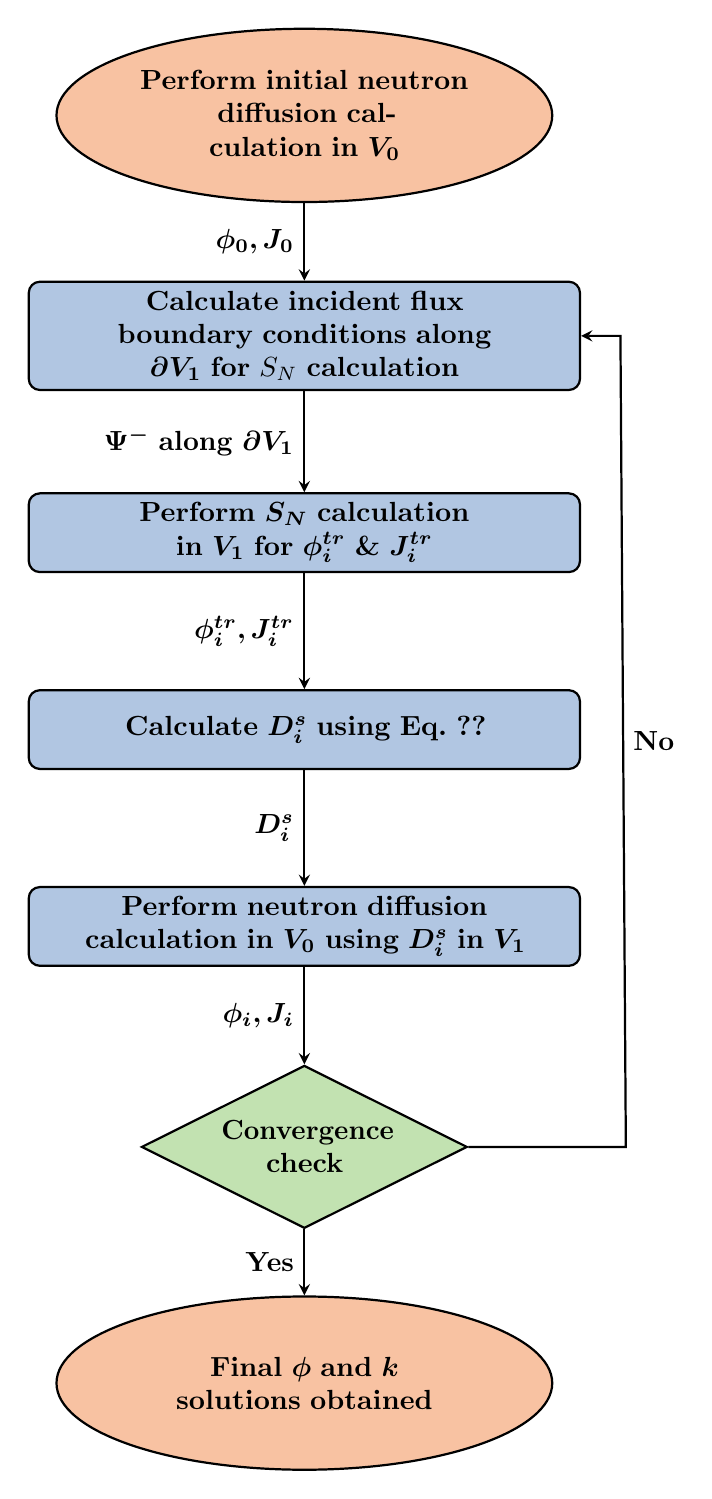
\begin{tikzpicture}
    \node (1) [object] {\textbf{Perform initial neutron\\diffusion calculation in $\bm{V_0}$}};
    \node (2) [process, below of=1, yshift=-1.8cm]
      {\textbf{Calculate incident flux boundary conditions along\\$\bm{\partial V_1}$ for $S_N$ calculation}};
    \node (3) [process, below of=2, yshift=-1.5cm]
      {\textbf{Perform $\bm{S_N}$ calculation\\in $\bm{V_1}$ for $\bm{\phi^{tr}_i}$ \& $\bm{J^{tr}_i}$}};
    \node (4) [process, below of=3, yshift=-1.5cm]
      {\textbf{Calculate $\bm{D^s_i}$ using Eq.\ \ref{eq:svdc}}};
    \node (5) [process, below of=4, yshift = -1.5cm]
      {\textbf{Perform neutron diffusion\\calculation in $\bm{V_0}$ using $\bm{D^s_i}$ in $\bm{V_1}$}};
    \node (6) [decision, below of=5, yshift = -1.8cm]
      {\textbf{Convergence\\check}};
    \node (7) [object, below of=6, yshift = -2cm]
      {\textbf{Final $\bm{\phi}$ and $\bm{k}$\\solutions obtained}};
    \draw [arrow] (1) -- node[anchor=east] {$\bm{\phi_0, J_0}$} (2);
    \draw [arrow] (2) -- node[anchor=east] {$\bm{\Psi^-}$ \textbf{along} $\bm{\partial V_1}$} (3);
    \draw [arrow] (3) -- node[anchor=east] {$\bm{\phi^{tr}_i, J^{tr}_i}$} (4);
    \draw [arrow] (4) -- node[anchor=east] {$\bm{D^s_i}$} (5);
    \draw [arrow] (5) -- node[anchor=east] {$\bm{\phi_i, J_i$}} (6);
    \draw [arrow] (6) -- node[anchor=east] {\textbf{Yes}} (7);
    \draw [arrow] (6) -- ([shift={(2cm,0cm)}]6.east)-- node[anchor=west] {\textbf{No}} ([shift={(0.5cm,0cm)}]2.east)--(2);
  \end{tikzpicture}
  \caption{Algorithm flowchart for the hybrid $S_N$-diffusion method.}
  \label{fig:algorithm}
\end{figure}

\subsubsection{$S_N$ Subsolver Boundary Conditions \& Buffer Zone}

The main challenge lies in determining appropriate boundary conditions for the $S_N$ subproblem.
Given that we want to limit the coverage of $V_1$ to the control rod region and its
immediate vicinity, $V_1$ should be sufficiently smaller than $V_0$, but large enough to capture
anisotropies in the flux due to the control rod. As a consequence, the boundaries $\partial V_1$ 
lie well within $V_0$. Crucially, there is currently no feasible method of generating
accurate boundary fluxes for an $S_N$ solver from a neutron diffusion flux solution. In 1-D, the
standard one-group $S_N$ method requires N/2
incoming boundary flux parameters per boundary mesh point for the N/2 neutron angular fluxes
flowing into $V_1$. The neutron diffusion method can produce at most one independent
incoming flux parameter per mesh point; this parameter is the neutron forward/backward current in
the $P_1$ approximation defined as:
%
\begin{align}
  J_{g,\pm} &= \frac{\phi_g}{4} \mp \frac{D_g}{2}\frac{d\phi_g}{dx} \label{eq:p1-j}
  \shortintertext{where}
  J_{g,\pm} &= \mbox{ neutron forward/backward current of group }g. \nonumber
\end{align}
%
Without additional information, the next best estimate is a uniformly
isotropic transmission of angular flux, i.e., all N/2 incoming angular fluxes $\Psi$ are equal in
magnitude. This is a good assumption far from the control rod, but will not produce accurate
fluxes if the boundary is too close to the control rod. This type of boundary condition is similar
to the white boundary condition, which describes the uniformly
isotropic reflection of particles at a boundary, except this case involves transmission rather than
reflection. Isotropic flux transmission at $x$ can be expressed mathematically for forward angular
fluxes as:
%
\begin{align}
  \sum^N_{n=N/2+1}w_n\mu_n\Psi(x,\mu_n) =& J_{+}(x) && (\mu_n>0) \nonumber \\
  \Psi(x,\mu_n)\sum^N_{n=N/2+1}w_n\mu_n =& J_{+}(x) && (\because \mbox{isotropic transmission})
  \nonumber \\
  \Psi(x,\mu_n) =& J_{+}(x)\Bigg/\sum^N_{n=N/2+1}w_n\mu_n
\end{align}
%
and backward angular fluxes as:
%
\begin{align}
  \sum^{N/2}_{n=1}w_n\mu_n\Psi(x,\mu_n) =& J_{-}(x) && (\mu_n<0) \nonumber \\
  \Psi(x,\mu_n)\sum^{N/2}_{n=1}w_n\mu_n =& J_{-}(x) && (\because \mbox{isotropic transmission})
  \nonumber \\
  \Psi(x,\mu_n) =& J_{-}(x)\Bigg/\sum^{N/2}_{n=1}w_n\mu_n \label{eq:sn-psi-j}
\end{align}
%
These boundary conditions for the $S_N$ sub-solver will generally yield some deviations in the
$\phi$ distributions since neutron fluxes in realistic reactor systems are at least slightly
anisotropic in most of the domain. However, in my preliminary investigations, the influence of
boundary conditions on the ratio $J$ and $\frac{d\phi}{dx}$ does not extend far from the boundaries
in optically thick media due to the strong scattering (e.g., graphite or molten salt) or
absorption effects (e.g., control rod). In the bulk regions far from the boundaries, the
scattering and absorption effects have the most significant influence on the flux. I observed that
the \glspl{SVDC} generated with the $S_N$ sub-solver within $V_1$ were accurate everywhere except
near $\partial V_1$. Therefore, $V_1$ must be large enough to provide transport corrections
through the \glspl{SVDC} and accommodate inaccurate \glspl{SVDC} near
$\partial V_1$. The inaccurate \glspl{SVDC} should then be discarded in favor of using
$P_1$-based diffusion coefficients as in the rest of $V_0$ not covered by $V_0$. The
subsequent neutron diffusion calculation with this mix of \glspl{SVDC} and $P_1$-based diffusion
coefficients should provide more accurate $\phi$ and $k$ estimates than a conventional
neutron diffusion calculation.

%To resolve this issue, I posit the following hypothesis: \textit{If there exists a highly
%neutron-absorbing control rod region within the $S_N$ subproblem domain $V_1$ and the $S_N$
%subproblem boundary $\partial V_1$ lies several neutron mean free paths away from this
%region, the \gls{SVDC} values calculated near the control rod region (using the $S_N$ sub-solver
%with isotropic hemisphere boundary conditions) will tend to the actual flux gradient solution
%(using a reference $S_N$ calculation across the entire problem domain $V$).} In other words,
%suboptimal boundary conditions may induce inaccurate \gls{SVDC} values near the $\partial
%V_1$ subdomain boundaries, but the \gls{SVDC} values further from $\partial V_1$ are
%accurate and very weakly dependent on the boundary conditions. These inaccurate \gls{SVDC} values
%close to $V_1$ may be discarded in favor of the default $P_1$-based diffusion coefficients.
%I will refer to the region containing these discarded values as the \textit{dead zone} or
%$V_2$, where $V_2 \subset V_1 \subseteq V_0$.

\subsubsection{Hybrid Method Verification with Case 0}

In this subsection, I revisit Case 0
(Figure \ref{fig:case-0-geom}) to test my hypothesis and demonstrate the hybrid $S_N$-diffusion
method. Once more, I defer general numerical implementation details to
Section \ref{sec:implementation}.

In Section \ref{sec:svdc}, the \gls{SVDC} generated from the reference $S_8$ calculation exhibited
significant spatial variations attributed to the presence of the control rod, as shown in Fig
\ref{fig:c0diffcoef}. The group 1 and 2 \gls{SVDC} values approach asymptotic values near the
corresponding group 1 and 2 $P_1$-based diffusion coefficient values near $x=15$ cm and $x=5$ cm,
respectively. Therefore, the $V_1$ should, at minimum, cover the domain between $x=0$ cm and
$x=15$ cm. Allowing for a buffer region for inaccurate \glspl{SVDC} near $\partial V_1$, I
defined $V_1$ to span from $x=0$ cm to $x=17.5$ cm.

I set up the hybrid method to automatically determine the cutoff point, beyond which \glspl{SVDC}
in $V_1$ are discarded, based on the \gls{SVDC} distribution generated in every iteration.
Starting from the interface between the control rod and fuel-graphite region, the algorithm sweeps
rightward for the point at which the group-wise \gls{SVDC} distribution approaches within 1\% of
the $P_1$-based diffusion coefficient value. This point serves as the cutoff point. The hybrid
method converges rapidly within two outer iterations comprising three neutron diffusion and two
$S_8$ calculations in total as outlined by the hybrid method algorithm; the change in $k$ between
the second and third outer iterations is approximately $10^{-7}$.
%
\begin{figure}[htb!]
  \centering
  \begin{subfigure}[b]{.49\textwidth}
    \centering
    \includegraphics[width=\textwidth]{case-0-group-1-hybrid-diffcoef}
    \caption{Group 1}
    \label{fig:c0g1hd}
  \end{subfigure}
  \hfill
  \begin{subfigure}[b]{.49\textwidth}
    \centering
    \includegraphics[width=\textwidth]{case-0-group-2-hybrid-diffcoef}
    \caption{Group 2}
    \label{fig:c0g2hd}
  \end{subfigure}
  \caption{$P_1$-based flux-limited diffusion coefficient and \gls{SVDC} spatial distribution for
  Case 0. The \gls{SVDC} distributions were generated from the reference $S_8$ (``SVDC'') and the
  hybrid (``Hybrid'') calculations.}
  \label{fig:c0hd}
\end{figure}

Refer to Figures \ref{fig:c0g1hd} and \ref{fig:c0g2hd} for a qualitative comparison of group 1 and
2 $P_1$-based diffusion coefficients, \glspl{SVDC} derived from the reference $S_8$ calculation as
demonstrated in Section \ref{sec:svdc}, and \glspl{SVDC} derived from the hybrid $S_N$-diffusion
method discussed here. The \glspl{SVDC} from the hybrid method agree well with the reference
\glspl{SVDC} in the control rod region and for most of the fuel-graphite region up to around
$x=15$ cm. Both sets of \glspl{SVDC} approximately coincide with the $P_1$ diffusion coefficient
values within 1\% difference from $x=14.615$ cm and $x=3.390$ cm onwards for group 1 and
group 2, respectively. Accordingly, the buffer region spans from $x=14.615$ cm to $x=17.500$ cm for
group 1 and $x=3.390$ cm to $x=17.500$ cm for group 2, in which the hybrid method defaults to the
$P_1$-based diffusion coefficients. Given that the reference \gls{SVDC} values will generally not
be known in real-world problems, the hybrid method relies on finding the intersection point of the
\gls{SVDC} and $P_1$ diffusion coefficient values to determine the buffer region cutoff point. The
size of $V_1$ will also have to be based on where this intersection point lies.
Another important consideration is the fact that the neutron flux gradient will be discontinuous if
the \gls{SVDC} and $P_1$ diffusion coefficient values are too far apart in magnitude at the buffer
region cutoff point. A flux gradient discontinuity in a homogeneous bulk region is non-physical and
unacceptable. In Section \ref{sec:prelim-results}, I study \gls{SVDC} distribution trends
in more heterogeneous systems and their implications on determining the size of $V_1$ and
the cutoff point.
%
\begin{figure}[htb!]
  \centering
  \begin{subfigure}[b]{.49\textwidth}
    \centering
    \includegraphics[width=\textwidth]{case-0-group-1-hybrid-flux}
    \caption{Group 1}
    \label{fig:c0g1hf}
  \end{subfigure}
  \hfill
  \begin{subfigure}[b]{.49\textwidth}
    \centering
    \includegraphics[width=\textwidth]{case-0-group-2-hybrid-flux}
    \caption{Group 2}
    \label{fig:c0g2hf}
  \end{subfigure}
  \caption{Neutron group 1 and 2 flux distributions from the diffusion, $S_8$, reference
  \gls{SVDC}, and hybrid methods for Case 0.}
  \label{fig:c0hf}
  \centering
  \begin{subfigure}[b]{.49\textwidth}
    \centering
    \includegraphics[width=\textwidth]{case-0-group-1-hybrid-flux-diff}
    \caption{Group 1}
    \label{fig:c0g1hfdiff}
  \end{subfigure}
  \hfill
  \begin{subfigure}[b]{.49\textwidth}
    \centering
    \includegraphics[width=\textwidth]{case-0-group-2-hybrid-flux-diff}
    \caption{Group 2}
    \label{fig:c0g2hfdiff}
  \end{subfigure}
  \caption{Difference in neutron group 1 and 2 flux distributions from the diffusion,
  diffusion-\gls{SVDC}, and hybrid methods with respect to the $S_8$ flux distribution for Case 0.}
  \label{fig:c0hfdiff}
\end{figure}

Figures \ref{fig:c0g1hf} and \ref{fig:c0g2hf} show the group 1 and 2 neutron flux distributions
from the various methods, while Figures \ref{fig:c0g1hfdiff} and \ref{fig:c0g2hfdiff} show the
difference in flux with respect to the $S_8$ flux distribution. As
expected following the diffusion coefficient discussion, the hybrid method flux distribution
matches the $S_8$ and Diffusion-\gls{SVDC} flux distributions well. The $k$ estimate from the
hybrid method is 0.62774, which is only 0.00024 higher than the Diffusion-\gls{SVDC} method, and
0.00038 higher than the $S_8$ method.

In Case 0, $V_1$ covers more than half of $V_0$ due to the control rod region being
the only significant source of influence on the neutron flux distribution in the
otherwise homogeneous system with reflective boundary conditions. I chose Case 0 as a simple test
case to aid in introducing the hybrid $S_N$-diffusion method. In Section \ref{sec:prelim-results},
I present more results with the hybrid method on more complicated geometries containing neutron
reflector, air, and heterogeneous fuel-graphite lattice regions and vacuum boundary conditions. In
these other test cases, the hybrid method yields smaller $V_1$-to-$V_0$ ratios,
reducing computational costs from running $S_N$ calculations over a relatively smaller
region.

\section{Numerical Implementation} \label{sec:implementation}

In Section \ref{sec:theory}, I presented the theoretical basis for the hybrid
$S_N$-diffusion method and demonstrated the method on a simple problem. Now I will discuss
numerical implementation details of group
constant data processing and the neutron diffusion, $S_N$ neutron transport, and hybrid
$S_N$-diffusion solvers. I implemented all numerical solvers and analysis scripts in the Python
programming language. First, I will discuss the material group constant data generation and
postprocessing steps. Next, I present the implementation details of the neutron
diffusion and $S_N$ numerical methods. Lastly, I present how they are coupled to form the hybrid
$S_N$-diffusion method.

\subsection{Group Constant Data Generation}

The group constants required by either or both neutron diffusion and $S_N$ neutron transport
methods are:
%
\begin{itemize}
  \item $\Sigma_{t,g}$: Macroscopic total cross section in group $g$,
  \item $\Sigma_{r,g}$: Macroscopic removal cross section in group $g$,
  \item $\Sigma_s^{g'\rightarrow g}$: Macroscopic group-to-group scattering cross section matrix,
  \item $\Sigma_{s,l}^{g'\rightarrow g}$: $l$-th Legendre moment of the macroscopic
    group-to-group scattering cross section matrix,
  \item $\Sigma_{sp,l}^{g'\rightarrow g}$: $l$-th Legendre moment of the macroscopic
    group-to-group scattering production cross section matrix,
  \item $D_g$: $P_1$-based diffusion coefficient in group $g$,
  \item $\nu\Sigma_{f,g}$: Product of the average number of neutrons produced per fission and the
    macroscopic fission cross section in group $g$,
  \item $\chi_g$: Neutron fission spectrum in group $g$.
\end{itemize}
%
These group constants are generated using OpenMC's multigroup cross section generation capability
\cite{boyd_multigroup_2019} and postprocessed using a Python script into JSON format files.
$\Sigma_{r,g}$ is the only quantity that OpenMC does not directly provide. It is calculated as
%
\begin{align}
  \Sigma_{r,g} =& \sum^G_{g'\neq g}\Sigma_s^{g\rightarrow g'}+\Sigma_{a,g}-\left(\Sigma_{sp}^{g
    \rightarrow g} - \Sigma_s^{g\rightarrow g}\right)
  \shortintertext{where}
      \Sigma_{a,g} =& \mbox{ macroscopic absorption cross section in group $g$,} \nonumber \\
      \Sigma_{sp}^{g\rightarrow g} =& \mbox{ macroscopic scattering production cross section from
      group $g$ to $g$.} \nonumber
\end{align}
%
$\Sigma_{r,g}$ primarily represents the loss of neutrons from group $g$ through outscattering and
absorption. $\Sigma_{sp}^{g\rightarrow g}$ incorporates neutron multiplication effects from neutron
knockout reactions into the scattering cross section. Neutron knockout reactions are commonly
tallied as scattering reactions, and $\Sigma_{r,g}$ is a convenient term to
incorporate neutron knockout effects into the neutron diffusion equations. I ran all test cases for
$S_N$ and hybrid method calculations with up to the 2nd Legendre moments of the scattering
cross sections ($L=2$).

OpenMC uses the $P_1$ flux-limited formulation \cite{pomraning_flux-limited_1984} for calculating
$D_g$ as follows
%
\begin{align}
  D_g =& \frac{1}{3\Sigma_{tr,g}},
  \shortintertext{where}
  \Sigma_{tr,g} =& \frac{\langle\Sigma_{t,g}\phi_g\rangle-\langle\Sigma_{s1,g}\phi_g\rangle}
  {\langle\phi_g\rangle}, \nonumber \\
  \langle\Sigma_{t,g}\phi_g\rangle =& \int_{r\in V}dr \int_{4\pi}d\Omega\int^{E_{g-1}}_{E_g}dE\
  \Sigma_{t,g}(r,E)\Psi(r,E,\Omega), \nonumber \\
  \langle\Sigma_{s1,g}\phi_g\rangle =& \int_{r\in V}dr \int_{4\pi}d\Omega\int^{E_{g-1}}_{E_g}dE
  \int_{4\pi}d\Omega'\int^{\infty}_0dE'\int^1_{-1}d\mu\ \mu\Sigma_s(r,E'\rightarrow E,\Omega'\cdot
  \Omega)\phi(r,E',\Omega'), \nonumber \\
  \langle \phi \rangle =& \int_{r\in V}dr\int_{4\pi}d\Omega\int^{E_{g-1}}_{E_g}dE\ \Psi(r,E,\Omega)
  .\nonumber
\end{align}

\subsection{Neutron Diffusion Method}

On a 1-D uniform spatial grid with $I+1$ mesh points, the neutron scalar flux variables
$\phi_{g,i}$ are defined on the mesh points $x_i$. Theoretically, group constants are volumetric
material properties that should be defined on the cell-centered half-integer mesh points
$x_{i+\sfrac{1}{2}}$. In practice, all material properties except diffusion coefficients are
uniform in each subregion and sampled at $x_i$. To avoid ambiguity concerning diffusion
coefficient sampling, I formulated all test cases such that all material interfaces fall on $x_i$.

Discretizing the multigroup $k$-eigenvalue neutron diffusion equations in Eq.\ \ref{eq:1d-diff}
and reformulating the scattering term using neutron balance in the control volume bounded by
$x_{i-\sfrac{1}{2}}$ and $x_{i+\sfrac{1}{2}}$ yields
%
\begin{align}
  J_{g,i+\sfrac{1}{2}} - J_{g,i-\sfrac{1}{2}} + \Sigma_{t,g,i} \phi_{g,i} \Delta x = \sum^G_{g'=1}\left[
  \Sigma_{s,i}^{g'\rightarrow g}\phi_{g',i} + \chi_{g,i}\frac{\nu\Sigma_{f,g',i}}{k} \phi_{g',i}
\right]\Delta x. \label{eq:diff-j}
\end{align}
%
Using the diamond difference scheme to replace the $J$ terms with the discretized form of
Fick's first law of diffusion,
%
\begin{align}
  J_{g,i+\sfrac{1}{2}} = -D_{g,i+\sfrac{1}{2}}\frac{d\phi_{g,i+\sfrac{1}{2}}}{dx} =
  -D_{g,i+\sfrac{1}{2}} \frac{\phi_{g,i+1}-\phi_{g,i}}{\Delta x},
\end{align}
%
and rearranging the terms in Eq.\ \ref{eq:diff-j} yields
%
\begin{align}
  -\frac{D_{g,i-\sfrac{1}{2}}}{\Delta x} \phi_{g,i-1} + &\left[\frac{D_{g,i-\sfrac{1}{2}}+
  D_{g,i+\sfrac{1}{2}}}{\Delta x} + \Delta x\ \Sigma_{r,g,i} \right]\phi_{g,i} -
  \frac{D_{g,i+\sfrac{1}{2}}}{\Delta x}\phi_{g,i+1} -\Delta x\sum^G_{g'\neq g}
  \Sigma_{s,i}^{g'\rightarrow g}\phi_{g',i} \nonumber \\
  =& \Delta x\sum^G_{g'=1}
  \chi_{g,i} \frac{\nu\Sigma_{f,g',i}}{k} \phi_{g',i}, \label{eq:diff-fd}
  \shortintertext{where}
  \Sigma_{r,g} =& \Sigma_{t,g} - \Sigma_s^{g\rightarrow g} \nonumber \\
  =& \mbox{ macroscopic removal cross section for neutron group }g. \nonumber
\end{align}
%
The diamond difference scheme is 2nd-order accurate, and this form is
equivalent to applying 2nd-order finite differencing to the original neutron diffusion equation in
Eq.\ \ref{eq:1d-diff} with diamond differencing for the cell-centered group constants.
The fixed neutron source $S_g$ is ignored here since the test cases are all neutron-multiplying
systems with no fixed source.

I implemented two types of boundary conditions: vacuum and reflective boundary conditions. The
\textbf{vacuum boundary conditions} are imposed by setting the incoming flux in the $P_1$
approximation to zero and applying 2nd-order finite differencing as follows:
%
\begin{align}
  \mbox{Left boundary: } \frac{\phi_{g,0}}{4}-\frac{D_{g,\sfrac{1}{2}}}{2}
  \frac{\left(-\phi_{g,2}+4\phi_{g,1}-3\phi_{g,0}\right)}{2\Delta x} =& 0 \\
  \mbox{Right boundary: } \frac{\phi_{g,I}}{4}+\frac{D_{g,I-\sfrac{1}{2}}}{2}
  \frac{\left(\phi_{g,I-2}-4\phi_{g,I-1}+3\phi_{g,I}\right)}{2\Delta x} =& 0.
\end{align}
%
The \textbf{reflective boundary conditions} are imposed by setting the flux gradient to zero and
applying 2nd-order finite differencing as follows:
%
\begin{align}
  \mbox{Left boundary: } \frac{-3\phi_{g,0}+4\phi_{g,1}-\phi_{g,2}}{2\Delta x} =& 0 \\
  \mbox{Right boundary: } \frac{3\phi_{g,I}-4\phi_{g,I-1}+\phi_{g,I-2}}{2\Delta x} =& 0
\end{align}
%
At material interfaces, the continuity condition requires that the net neutron current on either
side of the interface be equal as follows:
%
\begin{align}
  -\frac{3D_{g,i-\sfrac{1}{2}} - D_{g,i-\sfrac{3}{2}} }{2}
  \frac{\phi_{g,i-2}-4\phi_{g,i-1}+3\phi_{g,i}}{2\Delta x} =&
  -\frac{3D_{g,i+\sfrac{1}{2}} - D_{g,i+\sfrac{3}{2}} }{2}
  \frac{-3\phi_{g,i}+4\phi_{g,i+1}-\phi_{g,i}}{2\Delta x} \label{eq:itf-bc}
\end{align}
%
for a material interface at $x_i$.

Altogether, they form a system of equations of the form $\bm{A\overline{\phi}}=\bm{\frac{1}{k}
B\overline{\phi}}$, where $\bm{\overline{\phi}}$ is a flattened vector representation of
$\phi_{g,i}$, and $\bm{A}$ and $\bm{B}$ are matrices of the coefficients of $\phi_{g,i}$ as given
by Eqs. \ref{eq:diff-fd} to \ref{eq:itf-bc}. I implemented the inverse power method to find $k$ and
$\overline{\phi}$. The inverse power method algorithm is as follows
%
\begin{align}
  \shortintertext{1. Initialize $k^0$ and $\bm{\overline{\phi}}^0$}
  \shortintertext{2. Update $\bm{\overline{\phi}}$ and $k$}
  \bm{\overline{\phi}}^m =& \frac{1}{k^{m-1}}\bm{A}^{-1}\bm{B\overline{\phi}}^{m-1} \\
  k^m =& k^{m-1}\frac{|\bm{B\overline{\phi}}^m|}{|\bm{B\overline{\phi}}^{m-1}|}
  \shortintertext{3. Check whether convergence is reached}
  \epsilon_\phi =
  \frac{|\bm{\overline{\phi}}^m-\bm{\overline{\phi}}^{m-1}|}{|\bm{\overline{\phi}}^m|} <& \
  tol_{\bm{\overline{\phi}}} \\
  \epsilon_k =
  \frac{|k^m-k^{m-1}|}{|k^m|} <& \ tol_k
  \shortintertext{4. Return to Step 2 if either expression is false, otherwise exit.} \nonumber
\end{align}
%
$k^m$ and $\overline{\phi}^m$ denote estimates of $k$ and $\overline{\phi}$ after the $m$-th
iteration. Matrix $\bm{A}$ is a primarily tridiagonal matrix with at most $G-1$ off-diagonal terms
from the fourth term in Eq.\ \ref{eq:diff-fd}. Thus, $\bm{A}$ is initialized as a sparse matrix to
take advantage of the computationally efficient sparse matrix solver functions from the
\texttt{sparse} class of the \texttt{SciPy} \cite{virtanen_scipy_2020} Python library for
scientific and technical computing. Matrix $\bm{B}$
is never initialized explicitly as a matrix. Instead, the vector $\bm{b}=\bm{B\overline{\phi}}$ is
updated directly in every iteration. In this system of equations, $|\bm{b}|$ corresponds to the
total number of fission neutrons produced in the system for a given $\bm{\overline{\phi}}$. This
quantity is calculated using the \texttt{trapezoid} numerical integration function from
\texttt{SciPy} to estimate the integral value of the source term, $\nu\Sigma_{g,f}\phi_{g}$, in $x$
from the discrete flux values in $\bm{x}$. Finally, the final $\phi_{g,i}$ is normalized by a
factor of $|\bm{b}|/k$ (no. of source neutrons) to obtain the neutron scalar flux per source
neutron.

\subsection{$S_N$ Neutron Transport Method}

For the 1-D $S_N$ neutron transport method on the same uniform spatial grid with $I+1$ mesh points,
the neutron angular flux variables $\Psi_{g,i,n}=\Psi_g(x_i,\mu_n)$ are defined on the mesh points
$x_i$ while neutron scalar flux variables $\phi_{g,i\pm\sfrac{1}{2}}=\phi_g(x_{i\pm\sfrac{1}{2}})$
are defined on the half-integer mesh points $x_{i\pm\sfrac{1}{2}}$. All group constants are sampled
at $x_{i\pm\sfrac{1}{2}}$.

The $S_N$ equations are solved using the transport sweep method in which the algorithm ``sweeps''
through the spatial grid and sequentially updates $\Psi_{g,i,n}$. The algorithm sweep
direction follows the direction of neutron travel, i.e. it sweeps in the positive direction for
$\Psi_{g,i,n}$ with $\mu_n>0$ and vice versa. Doing otherwise is unphysical and causes numerical
instabilities.

Discretizing the multigroup $S_N$ neutron transport equations in Eq.\ \ref{eq:1d-sn} about
$x_{i+\sfrac{1}{2}}$ yields
%
\begin{align}
  \mu_n\frac{\Psi_{g,i+1,n}-\Psi_{g,i,n}}{x_{i+1}-x_i} + \Sigma_{t,g,i+\sfrac{1}{2}}
  \Psi_{g,i+\sfrac{1}{2},n} = q_{g,i+\sfrac{1}{2},n}
\end{align}
%
where $q_{g,i+\sfrac{1}{2},n}$ represents the combined scattering and fission neutron source term.
After expressing $\Psi_{g,i+\sfrac{1}{2}}$ as the average of $\Psi_{g,i+1,n}$ and $\Psi_{g,i,n}$
in the diamond difference scheme and rearranging the terms, we obtain
%
\begin{align}
  \Psi_{g,i+1,n} =& \frac{1-\Sigma_{t,g}\Delta x/2\mu_n}{1+
    \Sigma_{t,g}\Delta x/2\mu_n}\Psi_{g,i,n} +
    q\frac{\Delta x}{\mu_n\left(1+\Sigma_{t,g}\Delta x/2\mu_n\right)} \label{eq:sweep-right} &&
    (\mbox{for } \mu_n > 0)
\shortintertext{and}
  \Psi_{g,i,n} =& \frac{1+\Sigma_{t,g}\Delta x/2\mu_n}{1-
    \Sigma_{t,g}\Delta x/2\mu_n}\Psi_{g,i+1,n} -
    q\frac{\Delta x}{\mu_n\left(1-\Sigma_{t,g}\Delta x/2\mu_n\right)}. \label{eq:sweep-left} &&
    (\mbox{for } \mu_n < 0)
\end{align}
%
The remaining $i+\sfrac{1}{2}$ indexes on the group constants are dropped to reduce visual clutter.
These expressions are used to update $\Psi_{g,i,n}$ in the forward and backward transport sweeps.

The discretized scattering and fission terms in $q_{g,i+\sfrac{1}{2},n}$ are given as
%
\begin{align}
  q_{g,i+\sfrac{1}{2},n} =& \sum^G_{g'=1}\sum^L_{l=0}\frac{\left(2l+1\right)}
  {2}\Sigma_{s,l}^{g'\rightarrow g}P_l(\mu_n)\phi_{l,g',i+\sfrac{1}{2}} \nonumber \\
  &+\frac{\chi_g}{2}\sum^G_{g'=1}\frac{\nu\Sigma_{f,g'}}{k}\phi_{0,g',i+\sfrac{1}{2}}
  \label{eq:sn-q}
  \shortintertext{where}
  \phi_{l,g',i+\sfrac{1}{2}} =& \sum^N_{n'=1}w_{n'}P_l(\mu_{n'})\frac{\Psi_{g',i,n'}+
  \Psi_{g',i+1,n'}}{2}. \label{eq:phi-l}
\end{align}
%
$\phi_{l,g,i}$ are $l$-th Legendre expansions of the neutron flux evaluated using Gauss-Legendre
quadrature over $\mu_{n'}=[-1,1]$. $\phi_{0,g,i}$ and $\phi_{1,g,i}$ also correspond to the neutron
scalar flux $\phi_{g,i}$ and net current $J_{g,i}$, respectively.

For vacuum boundary conditions, $\Psi_{g,0,n}$ is zero for all positive $\mu_n$ while
$\Psi_{g,I,n}$ is zero for all negative $\mu_n$ as follows
%
\begin{align}
  \mbox{Left boundary: } \Psi_{g,0,n} =& 0 && (\mbox{for } \mu_n > 0) \\
  \mbox{Right boundary: } \Psi_{g,I,n} =& 0 && (\mbox{for } \mu_n < 0)
\end{align}
%
Reflective boundary conditions are imposed by equating the incoming angular flux to the
outgoing angular flux in the opposite direction as follows
%
\begin{align}
  \mbox{Left boundary: } \Psi_{g,0,n} =& \Psi_{g,0,n'} && (\mbox{for } \mu_n > 0, \mu_n =
  -\mu_{n'}) \\
  \mbox{Right boundary: } \Psi_{g,I,n} =& \Psi_{g,I,n'} && (\mbox{for } \mu_n < 0, \mu_n =
  -\mu_{n'})
\end{align}

The power iteration algorithm for the $S_N$ method is similar to the inverse power method algorithm
applied in the neutron diffusion method. The transport sweep step replaces the matrix-solving step
for updating $\overline{\phi}$.
%
\begin{align}
  \shortintertext{1. Initialize $k^0$, $\phi_{l,g,i+\sfrac{1}{2}}^0$, and $q^0$}
  \shortintertext{2. Apply transport sweeps to solve for $\Psi^m$ using Eqs. \ref{eq:sweep-right},
  \ref{eq:sweep-left}, and \ref{eq:sn-q}}
  \shortintertext{3. Update $\phi^m$ and $k^m$ using Eqs. \ref{eq:phi-l} and \ref{eq:sn-k}}
  k^m =& k^{m-1}\frac{\sum^I_{i=0}\sum^G_{g=1}\nu\Sigma_{f,g}\phi^m_{g,i+\sfrac{1}{2}}}
  {\sum^I_{i=0}\sum^G_{g=1}\nu\Sigma_{f,g}\phi^{m-1}_{g,i+\sfrac{1}{2}}} \label{eq:sn-k}
  \shortintertext{4. Check whether convergence is reached}
  \epsilon_\phi =
  \frac{|\bm{\overline{\phi}}^m-\bm{\overline{\phi}}^{m-1}|}{|\bm{\overline{\phi}}^m|} <& \
  tol_{\bm{\overline{\phi}}} \\
  \epsilon_k =
  \frac{|k^m-k^{m-1}|}{|k^m|} <& \ tol_k
  \shortintertext{5. Return to Step 2 if either expression is false, otherwise exit.} \nonumber
\end{align}

The transport sweep and $\phi^m$-update algorithms are parallelized using the \texttt{joblib}
parallel computing Python library \cite{noauthor_joblib_nodate} across all available CPU threads.
The total computational work is subdivided into several smaller tasks classified by unique pairs
of $g$ and $n$ values; each thread computes all $\Psi^m$ or $\phi^m$ values on the mesh for a given
pair of indexes $g$ and $n$.

\subsection{Hybrid $S_N$-Diffusion Method}

Without loss of generality, consider a 1-D system symmetric about the left boundary at $x_0=0$ cm.
In this case, as with Case 0, the control rod region is the left-most region, followed by other
regions. The $S_N$ subproblem domain $V_1$, containing the control rod and some region beyond it,
is bounded by $x_0$ and $x_j$ for some $x_j$
located several mean free paths to the right of the control rod region as governed by the relevant
discussion in Section \ref{sec:hybrid-method}.

Excluding the initial neutron diffusion calculation to initialize $k^0$ and $\phi^0$, each outer
iteration in the hybrid method consists of one $S_N$ neutron transport calculation and one neutron
diffusion calculation. The $\phi$ estimates from these $S_N$ transport and neutron diffusion
calculations are labeled as $\phi^{m+\sfrac{1}{2}}$ and $\phi^{m+1}$ during the
$(m+1)$-th outer iteration. $\phi^{m+\sfrac{1}{2}}$ spans $V_1$ while $\phi^{m+1}$ spans
the entire domain $V_0$.

For the $S_N$ subproblem boundary conditions, we discretize Eqs. \ref{eq:p1-j} and
\ref{eq:sn-psi-j} as follows
%
\begin{align}
  \Psi_{g,j,n} =& \frac{J_{g,-}(x_j)}{\sum^{N/2}_{n'=1}w_{n'}\mu_{n'}} \nonumber \\
  =& \frac{\frac{\phi_g(x_j)}{4}+
  \frac{D_g(x_{j-\sfrac{1}{2}})}{2}\frac{d\phi_g(x_j)}{dx}}{\sum^{N/2}_{n'=1}w_{n'}\mu_{n'}}
  \nonumber \\
  =& \frac{\frac{\phi_{g,j}}{4}+
  \frac{D_{g,j-\sfrac{1}{2}}}{2}\frac{\phi_{g,j}-\phi_{g,j-1}}{\Delta x}}
    {\sum^{N/2}_{n'=1}w_{n'}\mu_{n'}} && (\mu_n < 0) \label{eq:sn-bc}
\end{align}
%
where $D_g$ is the $P_1$-based diffusion coefficient value.

The \gls{SVDC} formulation in Eq.\ \ref{eq:svdc} is discretized using the diamond difference scheme
as follows
%
\begin{align}
  D^s_{g,i+\sfrac{1}{2}} =& -\frac{J^{tr}_{g,i+1}+J^{tr}_{g,i}}{2} \left(
  \frac{\phi^{tr}_{g,i+1}-\phi^{tr}_{g,i}}{\Delta x} \right)^{-1} = -\frac{\Delta x}{2}
  \frac{J^{tr}_{g,i+1}+J^{tr}_{g,i}}{\phi^{tr}_{g,i+1}-\phi^{tr}_{g,i}}. \label{eq:svdc-num}
\end{align}
%
%From Eq.\ \ref{eq:svdc-num}, we note that numerical instabilities may occur near flux peaks where
%the flux gradient and thus the denominator of Eq.\ \ref{eq:svdc-num} approach zero. On the other
%hand, this observation also implies that diffusion coefficient values have negligible influence on
%the flux solution near flux peaks due to the small flux gradient values. Therefore, we can avoid
%numerical instabilities by applying the following logic after calculating $D^s_g$: If the ratio of
%$|\frac{d\phi_g}{dx}|$ to $|\phi_g|$ is sufficiently small and $|D^s_g-D_g| > D_g$, the hybrid
%method defaults to using $D_g$ instead of $|D^s_g-D_g|$. The first conditional statement locates
%regions of relatively flat flux, and of these regions, the second conditional statement excludes
%regions which naturally experience flat flux such as air-filled regions. In all test cases,
%applying the first conditional as $|\frac{1}{\phi_g}\frac{d\phi_g}{dx}|<5\times 10^{-2}$ was
%sufficient for this task.

The hybrid $S_N$-diffusion algorithm is as follows
%
\begin{align}
  \shortintertext{1. Initialize $k^0$ and $\phi^0$ with an initial neutron diffusion calculation on
  $V_0$}
  \shortintertext{2. Generate estimates for $\Psi_{g,j,n}$ at $x_j$ for the $S_N$ transport
  calculation boundary conditions using Eq.\ \ref{eq:sn-bc}}
  \shortintertext{3. Calculate $\phi^{m+\sfrac{1}{2}}$ with the $S_N$ transport sub-solver on
  $V_1$}
  \shortintertext{4. Generate \glspl{SVDC} with $\phi^{m+\sfrac{1}{2}}$ and $J^{m+\sfrac{1}{2}}$
  using Eq.\ \ref{eq:svdc-num}}
  \shortintertext{5. Calculate $\phi^{m+1}$ with the newly generated \glspl{SVDC} and the neutron
  diffusion solver on $V_0$}
  \shortintertext{6. Check whether convergence is reached}
  \frac{|\bm{\overline{\phi}}^m-\bm{\overline{\phi}}^{m-1}|}{|\bm{\overline{\phi}}^m|} <& \
  tol_{\bm{\overline{\phi}}} \\
  \frac{|k^m-k^{m-1}|}{|k^m|} <& \ tol_k
  \shortintertext{7. Return to Step 2 if either expression is false, otherwise exit.} \nonumber
\end{align}
%
Generally, the convergence tolerance values for the outer hybrid method iteration must be smaller
than the tolerance values for the neutron diffusion and $S_N$ transport inner iterations. Using
$\phi^m$ from the neutron diffusion calculation as initial conditions for the $S_N$ transport
calculation in the $(m+1)$-th iteration helps to reduce the number of transport
sweeps required significantly.

The $S_N$ sub-solver only covers $V_1$, so it does not calculate an independent $k$
estimate. Instead, the $k^m$ from the neutron diffusion calculation scales the fission neutron
source term in the $S_N$ sub-solver.

%\section{Description of 1-D Test Cases} \label{sec:test-case}
%
%I designed ten 1-D test cases with increasing complexity to test the performance of the hybrid
%$S_N$-diffusion method in response to various geometrical features. The last two cases resemble the
%reference \gls{MSRE} design \cite{robertson_msre_1965}, which has centrally located control rods
%and air-filled rod guide tubes. Figure \ref{fig:case-geom} shows the geometries of Cases 0 to
%5b. All geometries have reflective boundary conditions at $x=0$ cm to reduce computational costs by
%creating half-core or repeating unit cell models. Cases 1a, 2a, 3a, and 4a are repeating unit
%cell models with reflecting boundaries on the right-side boundaries. Cases 1b, 2b, 3b, 4b, 5a, and
%5b are half-core models with vacuum boundaries on the right-side boundaries.
%
%Starting with an infinite, homogeneous region in Case 1a, I systematically added geometric
%complexities to each successive test case to identify how each feature impacts the neutronics
%results. Case 1b introduces a reflector region and vacuum boundary conditions relative to Case 1a.
%Cases 2a and 2b introduce a control rod region between $x=0$ cm and $x=0.5$ cm relative to Cases 1a
%and 1b. Cases 3a and 3b introduce a 0.5 cm-thick air gap between the control rod and the
%fuel-graphite mixture regions relative to Cases 2a and 2b. For Cases 4a and 4b, I replaced the
%homogeneous fuel-graphite mixture in Cases 1a and 2b with explicit fuel-graphite lattices, as shown
%in Figure \ref{fig:case-geom}. Case 5a introduces an air gap between the control rod and the
%fuel-graphite lattice regions. Lastly, Case 5b replaces the control rod region with an extended
%air gap region to provide a base case for the control rod worth calculations relative to Case 5a.
%
%The cases that do not contain control rod regions (1a, 1b, 4a, 4b, and 5b) serve as reference cases
%to quantify other sources of discrepancies in the neutron diffusion solution (e.g., geometrical
%heterogeneities, vacuum boundary condition approximation for neutron diffusion) and highlight how
%much the neutron diffusion method underperforms when the problem includes control rod regions.
%
%\begin{figure}[htb!]
%  \centering
%  \includegraphics[width=\columnwidth]{case-geometry}
%  \caption{Geometries of the 1-D test cases. The material labeled ``mixture'' represents a
%    homogeneous mixture of fuel and graphite at a ratio of 22.5\%-77.5\% by volume. All geometries
%    have reflective boundary conditions on the boundary at $x=0$ cm. The right-side boundaries are
%    reflective for Cases 1a, 2a, 3a, and 4a, and vacuum for Cases 1b, 2b, 3b, 4b, 5a, and 5b.}
%  \label{fig:case-geom}
%\end{figure}
%%
%\begin{figure}[htb!]
%  \centering
%  \begin{subfigure}[t]{.49\textwidth}
%    \centering
%    \includegraphics[width=\textwidth]{spectrum}
%    \caption{Neutron flux energy spectrum per source neutron}
%    \label{fig:spectrum}
%  \end{subfigure}
%  \hfill
%  \begin{subfigure}[t]{.49\textwidth}
%    \centering
%    \includegraphics[width=\textwidth]{reaction}
%    \caption{Flux-normalized scattering and absorption reaction rates}
%    \label{fig:reaction}
%  \end{subfigure}
%  \caption{Neutron flux energy spectrum and reaction rates for Case 5a. The dotted vertical lines
%  correspond to the discrete neutron energy group boundaries.}
%  \label{fig:spec-reac}
%\end{figure}
%%
%%\begin{table}[tb!]
%%  \centering
%%  \caption{Description of the 1-D Test Case Geometries.}
%%  \begin{tabular}{l c c c}
%%    \toprule
%%    Cases & Ordered list of regions & Ordered list of interface x-coordinates & Left \& Right BCs\\
%%    \midrule
%%    Case 0 & Control rod, homogenized fuel-graphite lattice &
%%    \bottomrule
%%  \end{tabular}
%%  \label{table:c0k}
%%\end{table}
%
%I ran all cases with four neutron energy groups. The list of energy group bounds are:
%$E=[10^{-5}, 10^0, 10^2, 10^5, 10^8]$ eV. Figures \ref{fig:spectrum} and \ref{fig:reaction} show
%how this energy group structure
%partitions the neutron flux energy spectrum and neutron reaction rates. For this preliminary work,
%the four-group structure is sufficient for showing different scattering and absorption trends of
%slow, intermediate, and fast neutrons. I also ran all cases on OpenMC to generate the required
%group constants and to assess the accuracy of the deterministic methods against OpenMC in
%continuous-energy (OpenMC-CE) and multigroup (OpenMC-MG) modes. Table \ref{table:var} shows how the
%position, direction of travel, neutron energy, and angle-dependence in $\Sigma_s$ are handled by
%OpenMC and the deterministic methods. Comparing OpenMC-MG results with OpenMC-CE results allows us
%to quantify errors arising from neutron energy group discretization and the scattering cross
%section simplifications. Each Monte Carlo simulation ran on 25 inactive and 125 active cycles of
%20,000 neutrons each, which sums up to 2.5 million tallied neutron histories.
%
%\begin{table}[tb!]
%  \centering
%  \footnotesize
%  \caption{Variable handling in OpenMC under continuous-energy (OpenMC-CE) and multigroup
%  (OpenMC-MG) modes, and in the $S_N$ neutron transport, neutron diffusion, and hybrid
%  $S_N$-diffusion methods. }
%  \begin{tabular}{c c c c c c}
%    \toprule
%    Variable & OpenMC-CE & OpenMC-MG & $S_N$ Transport & Diffusion & Hybrid \\
%    \midrule
%    Position, $\bm{r}$ & Continuous & Continuous & Discrete & Discrete & Discrete \\
%    Direction of travel, $\bm{\hat{\Omega}}$ & Continuous & Continuous & Discrete & N/A & N/A \\
%    Energy, $E$ & Continuous & Discrete & Discrete & Discrete & Discrete \\
%    Angle-dependence in $\Sigma_s$ & Continuous & 2nd Legendre moment & 2nd Legendre moment
%    & N/A & N/A \\
%    \bottomrule
%  \end{tabular}
%  \label{table:var}
%\end{table}
%
%\section{Simulation Parameters for Convergence} \label{sec:sim-param}
%
%The convergence of the results depends mainly on the following simulation parameters: mesh size
%($\Delta x$), convergence tolerance ($tol$), number of discrete ordinates ($N$), and the highest
%order moment of the scattering cross sections ($L$). The last two parameters apply only to $S_N$
%calculations. Table \ref{table:param} shows the values of simulation parameters applied to each
%method for the 1-D test cases.
%
%\begin{table}[tb!]
%  \centering
%  \footnotesize
%  \caption{Simulation parameters applied to the neutron diffusion, $S_N$, and hybrid
%  $S_N$-diffusion methods.}
%  \begin{tabular}{c c c c}
%    \toprule
%    Parameter & $S_N$ Transport & Neutron Diffusion & Hybrid $S_N$-Diffusion \\
%    \midrule
%    Mesh size, $\Delta x$ [cm]        & 0.0125    & 0.0125    & 0.0125 \\[.2cm]
%    \multirow{3}{*}{Convergence tolerance, $tol$}
%                                      &           &           & Diffusion: $10^{-6}$ \\
%                                      & $10^{-7}$ & $10^{-6}$ & $S_N$: $10^{-5}$ \\
%                                      &           &           & Outer: $10^{-3}$ \\[.2cm]
%    Discrete ordinates, $N$           & 8         & N/A       & 8 \\
%    Highest moment of $\Sigma^{g'\rightarrow g}_s$, $L$
%                                      & 2         & N/A       & 2 \\
%    \bottomrule
%  \end{tabular}
%  \label{table:param}
%\end{table}
%
%The simulation parameters did not show any significant correlation in the convergence tests. All
%three methods achieve reasonable convergence with $\Delta x=0.0125$ cm; halving the mesh size
%causes less than $30\times10^{-5}$ change in $k$ for the neutron diffusion and hybrid methods and
%less than $10^{-5}$ for the $S_8$ method. Further refinement of the $tol$, $N$, and $L$ parameters
%result in less than $2\times10^{-5}$
%change in $k$. The same $tol$ value applies to convergence checks for both $\phi$ and $k$ in all
%three methods because the variables converge at similar rates. The hybrid method requires three
%separate $tol$ values due to the inner and outer iterations. Notably, the hybrid method can reach
%convergence with a larger $tol$ value for its $S_N$ sub-solver than the $tol$ value for the
%standalone $S_N$ solver, which implies that $J$ and $\sfrac{d\phi}{dx}$ converge faster than $\phi$
%because the \glspl{SVDC} depend on those variables instead of $\phi$. Consequently, the $S_N$
%sub-solver requires much fewer iterations than the standalone $S_N$ solver. In combination with
%restricting $S_N$ calculations to the correction region, the hybrid method saves significant
%computation time compared to the standalone $S_N$ method.
%
%The outer iterations
%converge rapidly, so a $tol$ value of $10^{-3}$ is sufficient for convergence. The $\phi$ and $k$
%relative error norms ($\epsilon$) in all test cases decreased by two orders of magnitude on
%every outer iteration. For instance, Table \ref{table:epsilon} shows the $\epsilon$ values from the
%hybrid method after every outer iteration for Case 5a. The $\epsilon$ values fall below
%$10^{-5}$ by the 3rd and 4th iterations.
%
%\begin{table}[tb!]
%  \centering
%  \footnotesize
%  \caption{Relative error norm, $\epsilon$, values for $k$ and $\phi$ after each outer iteration in
%    the hybrid $S_N$-diffusion method for Case 5a.}
%  \begin{tabular}{c S[table-format=1.1e+1] S[table-format=1.1e+1]}
%    \toprule
%    Iteration   & {$\epsilon_k$}    & {$\epsilon_\phi$} \\
%    \midrule
%    1           & 1.6e-2            & 1.5e-2 \\
%    2           & 5.0e-5            & 4.7e-5 \\
%    3           & 1.4e-7            & 1.6e-7 \\
%    4           & 3.5e-9            & 1.4e-8 \\
%    \bottomrule
%  \end{tabular}
%  \label{table:epsilon}
%\end{table}
%
%
%\section{Results \& Discussion} \label{sec:prelim-results}
%
%In this section, I compare neutronics parameters for all test cases calculated from
%the OpenMC and deterministic methods. I refer to the OpenMC calculations under continuous-energy
%and multigroup modes as OpenMC-CE and OpenMC-MG, respectively. I did not apply the hybrid method to
%Cases 1a, 1b, 4a, 4b, and 5b, which serve as reference cases for how much the neutron diffusion
%method underperforms when control rod regions are present in the other cases.
%
%\subsection{Comparison of Multiplication factors, $k$}
%
%Tables \ref{table:ck1} and \ref{table:ck2} show all test case $k$ estimates from the OpenMC and
%deterministic methods. The tables also include statistical uncertainties for the OpenMC
%$k$ estimates.
%
%All five methods generally show reasonable agreement within each test case. The differences between
%the OpenMC-CE and OpenMC-MG $k$ estimates vary significantly from 0.00018 in Case 1a to 0.01622 in
%Case 4b. These Monte Carlo methods exhibit more significant differences in cases
%with vacuum boundary conditions (e.g., Cases 1b, 2b, 3b, 4b, 5a, 5b). These differences imply that
%the neutron energy discretization scheme must be revised to capture neutron leakage rates
%accurately. Beyond this preliminary study, I will explore better discrete energy group structures
%for further neutronics analyses of graphite-moderated \glspl{MSR}. For the rest of this
%section, I compare the $k$ estimates of the deterministic methods with OpenMC-MG.
%
%\begin{table}[htb!]
%  \centering
%  \footnotesize
%  \caption{Multiplication factor $k$ estimates for Cases 1a, 1b, 2a, 2b, 3a, and 3b from the
%    OpenMC-CE, OpenMC-MG, $S_8$ neutron transport, neutron diffusion, and hybrid $S_N$-diffusion
%    methods.}
%  \begin{tabular}{c S[table-format=1.5(2)] S[table-format=1.5(2)] S[table-format=1.5(2)]
%  S[table-format=1.5(2)] S[table-format=1.5(2)] S[table-format=1.5(2)]}
%    \toprule
%    \multirow{2}{*}{\textbf{Method}} &
%    \multicolumn{6}{c}{\textbf{Multiplication factor,} $\bm{k}$} \\
%    \cmidrule{2-7}
%    & {\textbf{Case 1a}} & {\textbf{Case 1b}} & {\textbf{Case 2a}} &
%    {\textbf{Case 2b}} & {\textbf{Case 3a}} & {\textbf{Case 3b}} \\
%    \midrule
%    OpenMC-CE & 1.60033(56) & 1.16749(60) & 1.20666(66) & 0.69499(47) & 1.19908(63) & 0.68565(53)\\
%    OpenMC-MG & 1.60015(33) & 1.18104(54) & 1.20570(66) & 0.70539(50) & 1.19976(48) & 0.69730(50)\\
%    $S_8$     & 1.60035     & 1.18068     & 1.20596     & 0.70470     & 1.19968     & 0.69652    \\
%    Diffusion & 1.60036     & 1.17932     & 1.19709     & 0.69274     & 1.19064     & 0.68450    \\
%    Hybrid    & {N/A}       & {N/A}       & 1.20630     & 0.70387     & 1.20004     & 0.69568    \\
%    \bottomrule
%  \end{tabular}
%  \label{table:ck1}
%\end{table}
%%
%\begin{table}[htb!]
%  \centering
%  \footnotesize
%  \caption{Multiplication factor $k$ estimates for Cases 4a, 4b, 5a, and 5b from the OpenMC-CE,
%    OpenMC-MG, $S_8$ neutron transport, neutron diffusion, and hybrid $S_N$-diffusion methods.}
%  \begin{tabular}{c S[table-format=1.5(2)] S[table-format=1.5(2)] S[table-format=1.5(2)]
%    S[table-format=1.5(2)]}
%    \toprule
%    \multirow{2}{*}{\textbf{Method}} &
%    \multicolumn{4}{c}{\textbf{Multiplication factor,} $\bm{k}$} \\
%    \cmidrule{2-5}
%    & {\textbf{Case 4a}} & {\textbf{Case 4b}} & {\textbf{Case 5a}} &
%    {\textbf{Case 5b}} \\
%    \midrule
%    OpenMC-CE & 1.64506(53) & 1.19116(63) & 0.70352(64) & 1.16832(58) \\
%    OpenMC-MG & 1.64355(37) & 1.20738(63) & 0.71396(50) & 1.18204(53) \\
%    $S_8$     & 1.64376     & 1.20744     & 0.71379     & 1.18218     \\
%    Diffusion & 1.64355     & 1.20811     & 0.70524     & 1.18274     \\
%    Hybrid    & {N/A}       & {N/A}       & 0.71673     & {N/A}       \\
%    \bottomrule
%  \end{tabular}
%  \label{table:ck2}
%\end{table}
%%
%\begin{table}[htb!]
%  \centering
%  \footnotesize
%  \caption{Differences in $k$ estimates for Cases 1a, 1b, 2a, 2b, 3a, and 3b for the $S_8$ neutron
%    transport, neutron diffusion, and hybrid $S_N$-diffusion methods relative to OpenMC-MG.}
%  \begin{tabular}{c S[table-format=+1.5(2)] S[table-format=+1.5(2)] S[table-format=+1.5(2)]
%      S[table-format=+1.5(2)] S[table-format=+1.5(2)] S[table-format=+1.5(2)]}
%    \toprule
%    \multirow{2}{*}{\textbf{Method}} & \multicolumn{6}{c}{$\bm{k-k_{MG}}$} \\
%    \cmidrule{2-7}
%    & {\textbf{Case 1a}} & {\textbf{Case 1b}} & {\textbf{Case 2a}} &
%    {\textbf{Case 2b}} & {\textbf{Case 3a}} & {\textbf{Case 3b}} \\
%    \midrule
%    $S_8$     & +0.00020(33) & -0.00036(54) & +0.00026(66) & -0.00069(50) & -0.00008(48) & -0.00078(50) \\
%    Diffusion & +0.00021(33) & -0.00172(54) & -0.00861(66) & -0.01265(50) & -0.00912(48) & -0.01280(50) \\
%    Hybrid    & {N/A}        & {N/A}        & +0.00060(66) & -0.00152(50) & +0.00028(48) & -0.00162(50) \\
%    \bottomrule
%  \end{tabular}
%  \label{table:ckdiff1}
%\end{table}
%%
%\begin{table}[htb!]
%  \centering
%  \footnotesize
%  \caption{Differences in $k$ estimates for Cases 4a, 4b, 5a, and 5b for the $S_8$ neutron
%    transport, neutron diffusion, and hybrid $S_N$-diffusion methods relative to OpenMC-MG.}
%  \begin{tabular}{c S[table-format=+1.5(2)] S[table-format=+1.5(2)] S[table-format=+1.5(2)]
%    S[table-format=+1.5(2)]}
%    \toprule
%    \multirow{2}{*}{\textbf{Method}} & \multicolumn{4}{c}{$\bm{k-k_{MG}}$} \\
%    \cmidrule{2-5}
%    & {\textbf{Case 4a}} & {\textbf{Case 4b}} & {\textbf{Case 5a}} &
%    {\textbf{Case 5b}} \\
%    \midrule
%    $S_8$     & +0.00021(37) & +0.00006(63) & -0.00017(50) & -0.00027(53) \\
%    Diffusion & +0.00000(37) & +0.00073(63) & -0.00872(50) & +0.00277(53) \\
%    Hybrid    & {N/A}        & {N/A}        & +0.00070(50) & {N/A}    \\
%    \bottomrule
%  \end{tabular}
%  \label{table:ckdiff2}
%\end{table}
%%
%\begin{table}[tb!]
%  \centering
%  \footnotesize
%  \caption{Control rod worths calculated as changes in the reactivity between Case 5a and 5b for
%    the OpenMC continuous-energy and multigroup mode calculations, and the $S_8$ neutron transport,
%  neutron diffusion, and hybrid $S_N$-diffusion methods.}
%  \begin{tabular}{c S}
%    \toprule
%    \multirow{2}{*}{\textbf{Method}} & {\textbf{Control rod worth}} \\
%                                     & {$\bm{\rho_{(5b)}-\rho_{(5a)}}$} \\
%    \midrule
%    OpenMC-CE & 0.56549(213) \\
%    OpenMC-MG & 0.55464(176) \\
%    $S_8$     & 0.55507 \\
%    Diffusion & 0.57246 \\
%    Hybrid    & 0.54974 \\
%    \bottomrule
%  \end{tabular}
%  \label{table:rod-worth}
%\end{table}
%
%Tables \ref{table:ckdiff1} and \ref{table:ckdiff2} show the differences in $k$ between OpenMC-MG
%and deterministic methods. The $k$ estimates from the $S_8$ neutron transport method show
%good agreement, with the estimates from OpenMC-MG with all pairs of $k$ values falling within
%1-2 standard deviations of each other. The only significant difference in implementation between
%the OpenMC-MG and $S_8$ methods is the discretization of the direction of travel variable
%$\hat{\Omega}$. The flux distributions exhibit more apparent differences, will be discussed in the
%following subsection. Nevertheless, the $S_8$ method is sufficiently accurate and consistent for
%modeling this graphite-moderated system with control rods.
%
%As expected, the neutron diffusion method performs significantly worse than the $S_8$ method in
%Cases 2, 3, and 5a, containing control rod regions. It deviates from the OpenMC-MG $k$
%estimate by up to -0.01280 in Case 3b compared to -0.00078 for the $S_8$ method. The hybrid method
%effectively improves the $k$ estimate to -0.00162 of the
%OpenMC-MG method for Case 3b. The hybrid method also appreciably improved the accuracy in all
%other applied cases.
%
%In a time-dependent multiphysics simulation involving rod
%insertion or withdrawal, the control rod worth determines the change in reactivity and the
%subsequent effects on the neutron flux and temperature distribution. I calculated the control rod
%worth by taking the change in reactivity $\rho$ between Case 5a and 5b for all five methods, as
%shown in Table \ref{table:rod-worth}. The formula for $\rho$ is given as
%%
%\begin{align}
%  \rho =& \frac{k-1}{k}.
%\end{align}
%%
%I took the $k$ estimate from the neutron diffusion method in Case 5b as the reference non-inserted
%case for the control rod worth calculation for the hybrid method. Compared with OpenMC-MG, the
%control rod worth from the neutron diffusion method deviates the most by 1782 pcm (percent mille)
%as opposed to 43 pcm and -490 pcm by the $S_8$ and hybrid methods, respectively.
%
%\subsection{Comparison of Neutron Flux Distributions, $\phi$}
%
%This section focuses on the neutron flux distributions in Cases 3b and 5a, representing the most
%complex geometries with homogeneous and lattice fuel-graphite regions. I sampled the flux
%distributions in OpenMC-CE and OpenMC-MG across coarser $0.1$-cm intervals to reduce the
%statistical uncertainties of each flux reading.
%
%\begin{figure}[htb!]
%  \centering
%  \begin{subfigure}[t]{.49\textwidth}
%    \centering
%    \includegraphics[width=\textwidth]{case-3b-group-1-flux}
%    \caption{Group 1}
%    \label{fig:c3bg1}
%  \end{subfigure}
%  \hfill
%  \begin{subfigure}[t]{.49\textwidth}
%    \centering
%    \includegraphics[width=\textwidth]{case-3b-group-2-flux}
%    \caption{Group 2}
%    \label{fig:c3bg2}
%  \end{subfigure}
%  \begin{subfigure}[t]{.49\textwidth}
%    \centering
%    \includegraphics[width=\textwidth]{case-3b-group-3-flux}
%    \caption{Group 3}
%    \label{fig:c3bg3}
%  \end{subfigure}
%  \hfill
%  \begin{subfigure}[t]{.49\textwidth}
%    \centering
%    \includegraphics[width=\textwidth]{case-3b-group-4-flux}
%    \caption{Group 4}
%    \label{fig:c3bg4}
%  \end{subfigure}
%  \caption{Neutron group flux distributions for Case 3b from OpenMC-CE, OpenMC-MG, $S_8$, neutron
%  diffusion, and hybrid methods.}
%  \label{fig:c3bflux}
%\end{figure}
%
%Figure \ref{fig:c3bflux} shows the neutron flux distributions for groups 1 to 4. Notably, the
%OpenMC-CE flux distribution is the most dissimilar, likely due to
%the inadequate neutron energy discretization scheme. Consequently, I compared the
%deterministic methods with OpenMC-MG to eliminate energy discretization errors. Figure
%\ref{fig:c3bfluxe} shows the relative differences in the flux distributions from $S_8$, neutron
%diffusion, and hybrid methods with respect to OpenMC-MG. The neutron diffusion method
%performs worse than $S_8$, especially near the control rod region between $x=0$ cm and $x=20$ cm
%for the slower group 3 and 4 neutron flux. Although the control rod region spans between $x=0$ cm
%and $x=0.5$ cm only, it induces strong flux gradients in its vicinity, thus rendering the neutron
%diffusion method less valid. The hybrid method significantly improves all four
%group fluxes in this region. Beyond $x=40$ cm, the neutron diffusion and hybrid methods produce
%similar flux error distributions due to the influence of the material interface between the
%fuel-graphite and reflector regions.
%
%\begin{figure}[htb!]
%  \centering
%  \begin{subfigure}[t]{.49\textwidth}
%    \centering
%    \includegraphics[width=\textwidth]{case-3b-group-1-flux-error}
%    \caption{Group 1}
%    \label{fig:c3bg1e}
%  \end{subfigure}
%  \hfill
%  \begin{subfigure}[t]{.49\textwidth}
%    \centering
%    \includegraphics[width=\textwidth]{case-3b-group-2-flux-error}
%    \caption{Group 2}
%    \label{fig:c3bg2e}
%  \end{subfigure}
%  \begin{subfigure}[t]{.49\textwidth}
%    \centering
%    \includegraphics[width=\textwidth]{case-3b-group-3-flux-error}
%    \caption{Group 3}
%    \label{fig:c3bg3e}
%  \end{subfigure}
%  \hfill
%  \begin{subfigure}[t]{.49\textwidth}
%    \centering
%    \includegraphics[width=\textwidth]{case-3b-group-4-flux-error}
%    \caption{Group 4}
%    \label{fig:c3bg4e}
%  \end{subfigure}
%  \caption{Relative differences of the neutron group flux distributions for Case 3b from the $S_8$,
%    neutron diffusion, and hybrid methods with respect to OpenMC-MG.}
%  \label{fig:c3bfluxe}
%\end{figure}
%
%For a quantitative assessment, I defined the normalized flux error $\varepsilon$ (not to be
%confused with relative error norm $\epsilon$) for each energy group with respect to the OpenMC-MG
%flux distribution using a normalized Frobenius/Euclidean norm formula given as
%%
%\begin{align}
%  \varepsilon_g =& \frac{\lVert\sum^I_{i=1}\phi_{g,i} - \phi^{MG}_{g,i}\rVert_F}
%  {\lVert\sum^I_{i=1}\phi^{MG}_{g,i}\rVert_F} =
%  \frac{\left[\sum^I_{i=1}\lvert\phi_{g,i} - \phi^{MG}_{g,i}\rvert^2 \right]^{\sfrac{1}{2}}}
%  {\left[\sum^I_{i=1}\lvert\phi^{MG}_{g,i}\rvert^2\right]^{\sfrac{1}{2}}}
%\end{align}
%%
%I integrated on the fine flux distributions over 0.1-cm intervals from $S_8$, neutron diffusion,
%and hybrid methods to match the 0.1-cm intervals of the OpenMC-MG flux distribution. Table
%\ref{table:c3berror} shows the $\varepsilon$ values for the deterministic methods. As expected,
%the hybrid method produces smaller flux error norms than the neutron diffusion method. The
%improvements are more pronounced for group 3 and 4 fluxes than group 1 and 2 fluxes.
%%
%\begin{table}[tb!]
%  \centering
%  \footnotesize
%  \caption{Normalized flux error $\varepsilon$ for Case 3b from the $S_8$, neutron diffusion, and
%    hybrid methods with respect to OpenMC-MG.}
%  \begin{tabular}{c S S S S}
%    \toprule
%    {\multirow{2}{*}{\textbf{Method}}} &
%    \multicolumn{4}{c}{\textbf{Normalized flux error,} $\bm{\varepsilon_g}$} \\
%    \cmidrule{2-5}
%    & {\textbf{Group 1}} & {\textbf{Group 2}} & {\textbf{Group 3}} &
%    {\textbf{Group 4}} \\
%    \midrule
%    $S_8$     & 0.0066 & 0.0048 & 0.0058 & 0.0067 \\
%    Diffusion & 0.0144 & 0.0147 & 0.0258 & 0.0267 \\
%    Hybrid    & 0.0122 & 0.0099 & 0.0087 & 0.0084 \\
%    \bottomrule
%  \end{tabular}
%  \label{table:c3berror}
%\end{table}
%
%Case 5a introduces significant geometrical heterogeneity from the fuel-graphite lattice region.
%The heterogeneity is very apparent from the flux distributions in Figure \ref{fig:c5aflux}. The
%OpenMC Monte
%Carlo methods captured the fluctuations in the flux through their continuous angle variable as
%opposed to the $S_8$, neutron diffusion, and hybrid methods. The group 1 flux peaks are notably
%pronounced since all fission neutrons are born in the fuel region, with the majority in group 1.
%Figure \ref{fig:c5afluxe} shows the relative differences in flux for the $S_8$, neutron diffusion,
%and hybrid methods relative to OpenMC-MG. All three methods show regular fluctuations in the
%relative flux differences corresponding to the fuel-graphite lattice. The $S_8$ method generally
%deviates the least from OpenMC-MG, while the neutron diffusion method exhibits
%significant flux deviations near the control rod region prior to $x=20$ cm and the material
%interface between the fuel and reflector regions beyond $x=40$ cm.
%
%\begin{figure}[htb!]
%  \centering
%  \begin{subfigure}[t]{.49\textwidth}
%    \centering
%    \includegraphics[width=\textwidth]{case-5a-group-1-flux}
%    \caption{Group 1}
%    \label{fig:c5ag1}
%  \end{subfigure}
%  \hfill
%  \begin{subfigure}[t]{.49\textwidth}
%    \centering
%    \includegraphics[width=\textwidth]{case-5a-group-2-flux}
%    \caption{Group 2}
%    \label{fig:c5ag2}
%  \end{subfigure}
%  \begin{subfigure}[t]{.49\textwidth}
%    \centering
%    \includegraphics[width=\textwidth]{case-5a-group-3-flux}
%    \caption{Group 3}
%    \label{fig:c5ag3}
%  \end{subfigure}
%  \hfill
%  \begin{subfigure}[t]{.49\textwidth}
%    \centering
%    \includegraphics[width=\textwidth]{case-5a-group-4-flux}
%    \caption{Group 4}
%    \label{fig:c5ag4}
%  \end{subfigure}
%  \caption{Neutron group flux distributions for Case 5a from OpenMC-CE, OpenMC-MG, $S_8$, neutron
%  diffusion, and hybrid methods.}
%  \label{fig:c5aflux}
%\end{figure}
%%
%\begin{figure}[htb!]
%  \centering
%  \begin{subfigure}[t]{.49\textwidth}
%    \centering
%    \includegraphics[width=\textwidth]{case-5a-group-1-flux-error}
%    \caption{Group 1}
%    \label{fig:c5ag1e}
%  \end{subfigure}
%  \hfill
%  \begin{subfigure}[t]{.49\textwidth}
%    \centering
%    \includegraphics[width=\textwidth]{case-5a-group-2-flux-error}
%    \caption{Group 2}
%    \label{fig:c5ag2e}
%  \end{subfigure}
%  \begin{subfigure}[t]{.49\textwidth}
%    \centering
%    \includegraphics[width=\textwidth]{case-5a-group-3-flux-error}
%    \caption{Group 3}
%    \label{fig:c5ag3e}
%  \end{subfigure}
%  \hfill
%  \begin{subfigure}[t]{.49\textwidth}
%    \centering
%    \includegraphics[width=\textwidth]{case-5a-group-4-flux-error}
%    \caption{Group 4}
%    \label{fig:c5ag4e}
%  \end{subfigure}
%  \caption{Relative differences of the neutron group flux distributions for Case 5a from the $S_8$,
%    neutron diffusion, and hybrid methods with respect to OpenMC-MG.}
%  \label{fig:c5afluxe}
%\end{figure}
%%
%\begin{table}[tb!]
%  \centering
%  \footnotesize
%  \caption{Normalized flux error $\varepsilon$ for Case 5a from the $S_8$, neutron diffusion, and
%    hybrid methods with respect to OpenMC-MG.}
%  \begin{tabular}{c S S S S}
%    \toprule
%    {\multirow{2}{*}{\textbf{Method}}} &
%    \multicolumn{4}{c}{\textbf{Normalized flux error,} $\bm{\varepsilon_g}$} \\
%    \cmidrule{2-5}
%    & {\textbf{Group 1}} & {\textbf{Group 2}} & {\textbf{Group 3}} &
%    {\textbf{Group 4}} \\
%    \midrule
%    $S_8$     & 0.0078 & 0.0074 & 0.0083 & 0.0085 \\
%    Diffusion & 0.0305 & 0.0202 & 0.0313 & 0.0406 \\
%    Hybrid    & 0.0290 & 0.0147 & 0.0143 & 0.0216 \\
%    \bottomrule
%  \end{tabular}
%  \label{table:c5aerror}
%\end{table}
%
%\subsection{Correction Regions \& Diffusion Coefficients}
%
%In this section, I compare the $P_1$-based diffusion coefficients, reference \glspl{SVDC}, and
%hybrid \glspl{SVDC} for Cases 3b and 5a. As in Section \ref{sec:hybrid-method}, the reference
%\glspl{SVDC} are derived from the $S_8$ flux solution, while the hybrid \glspl{SVDC} are derived
%from the $S_8$ sub-solver flux solution within the hybrid $S_N$-diffusion method.
%
%Figure \ref{fig:c3bdiffcoef} shows the various diffusion coefficient distributions for Case 3b
%between $x=0$ cm and $x=30$ cm. The figures omit the large diffusion coefficient values in the
%air gap region between $x=0.5$ cm and $x=1$ cm since they do not show any significant features. The
%hybrid \glspl{SVDC} closely match
%the reference \gls{SVDC} within most of the correction region, which terminates at $x=20$ cm.
%
%\begin{figure}[htb!]
%  \centering
%  \begin{subfigure}[t]{.49\textwidth}
%    \centering
%    \includegraphics[width=\textwidth]{case-3b-group-1-diffcoef}
%    \caption{Group 1}
%    \label{fig:c3bg1dc}
%  \end{subfigure}
%  \hfill
%  \begin{subfigure}[t]{.49\textwidth}
%    \centering
%    \includegraphics[width=\textwidth]{case-3b-group-2-diffcoef}
%    \caption{Group 2}
%    \label{fig:c3bg2dc}
%  \end{subfigure}
%  \begin{subfigure}[t]{.49\textwidth}
%    \centering
%    \includegraphics[width=\textwidth]{case-3b-group-3-diffcoef}
%    \caption{Group 3}
%    \label{fig:c3bg3dc}
%  \end{subfigure}
%  \hfill
%  \begin{subfigure}[t]{.49\textwidth}
%    \centering
%    \includegraphics[width=\textwidth]{case-3b-group-4-diffcoef}
%    \caption{Group 4}
%    \label{fig:c3bg4dc}
%  \end{subfigure}
%  \caption{$P_1$-based diffusion coefficient, reference \gls{SVDC}, and hybrid \gls{SVDC}
%    distributions for Case 3b between $x=0$ cm and $x=30$ cm.}
%  \label{fig:c3bdiffcoef}
%\end{figure}
%%
%\begin{figure}[htb!]
%  \centering
%  \includegraphics[width=.6\textwidth]{case-3b-grad-j}
%  \caption{The gradient of current $J$ in the homogeneous fuel-graphite mixture from $x=1$ cm to
%  $x=45$ cm for Case 3b.}
%  \label{fig:c3bgradj}
%\end{figure}
%
%We recall that the hybrid method determines cutoff points within the correction region where the
%\glspl{SVDC} coincide with the $P_1$-based diffusion coefficients so that the flux gradients
%remain continuous. The hybrid method discards \glspl{SVDC} in the buffer region between this
%cutoff point and the correction region boundary in favor of the $P_1$-based diffusion coefficients.
%Notably, the group 1 reference \glspl{SVDC} (Figure \ref{fig:c3bg1dc}) only coincides
%with the $P_1$-based diffusion coefficient after the vertical asymptotes where the flux
%gradient approaches zero. The trends in group 1 reference \glspl{SVDC} before and after the
%vertical asymptote imply that the \gls{SVDC} would have gradually approached the $P_1$-based
%diffusion coefficient value if the asymptote did not exist. Determining the cutoff point for the
%\glspl{SVDC} would have been problematic due to the vertical asymptote. However, the hybrid
%\glspl{SVDC} coincide with the $P_1$-based diffusion coefficients before the vertical asymptote.
%This behavior can be reliably reproduced in other geometries with large homogeneous fissile regions
%(Cases 2a, 2b, and 3a) as long as the correction region terminates near the neutron flux peaks.
%Nevertheless, the issue of handling vertical asymptotes in the \glspl{SVDC} has to be addressed
%since flux peaks and troughs will inevitably occur in more realistic reactor geometries.
%
%In contrast with the flux distributions in Figure \ref{fig:c3bflux}, the \gls{SVDC} distributions
%suggest that the control rod contributes to an extended range of transport corrections on group 1
%neutrons than the slower neutron groups. This phenomenon can be largely attributed to the highly
%non-uniform fission neutron source distribution, which serves as the only source of group 1
%neutrons in the absence of neutron up-scattering. The group 4 flux distribution
%significantly influences on fission neutron source distribution, leading to more group 1 neutrons
%being born closer to the reflector on the right than the
%control rod on the left. The biased neutron source distribution induces a highly non-linear neutron
%current distribution, as shown in Figure \ref{fig:c3bgradj}, and a departure from Fick's first law,
%which relates the current to the flux gradient. Therefore, the \gls{SVDC} distributions show that
%transport corrections to the faster neutron groups are as necessary for overall accuracy as
%transport corrections to the slower neutron groups.
%
%Figure \ref{fig:c5adiffcoef} shows the various diffusion coefficient distributions for Case 5a
%between $x=0$ cm and $x=30$ cm. As with Case 3b, the figures omit the large diffusion coefficient
%values in the air gap region between $x=0.5$ cm and $x=1.5$ cm  The hybrid \glspl{SVDC} closely match
%the reference \gls{SVDC} within most of the correction region, which terminates at $x=10$ cm.
%
%\begin{figure}[htb!]
%  \centering
%  \begin{subfigure}[t]{.49\textwidth}
%    \centering
%    \includegraphics[width=\textwidth]{case-5a-group-1-diffcoef}
%    \caption{Group 1}
%    \label{fig:c5ag1dc}
%  \end{subfigure}
%  \hfill
%  \begin{subfigure}[t]{.49\textwidth}
%    \centering
%    \includegraphics[width=\textwidth]{case-5a-group-2-diffcoef}
%    \caption{Group 2}
%    \label{fig:c5ag2dc}
%  \end{subfigure}
%  \begin{subfigure}[t]{.49\textwidth}
%    \centering
%    \includegraphics[width=\textwidth]{case-5a-group-3-diffcoef}
%    \caption{Group 3}
%    \label{fig:c5ag3dc}
%  \end{subfigure}
%  \hfill
%  \begin{subfigure}[t]{.49\textwidth}
%    \centering
%    \includegraphics[width=\textwidth]{case-5a-group-4-diffcoef}
%    \caption{Group 4}
%    \label{fig:c5ag4dc}
%  \end{subfigure}
%  \caption{$P_1$-based diffusion coefficient, reference \gls{SVDC}, and hybrid \gls{SVDC}
%    distributions for Case 5a between $x=0$ cm and $x=30$ cm.}
%  \label{fig:c5adiffcoef}
%\end{figure}
%
%Unlike Case 3b, the heterogeneous fuel-graphite lattice structure in Case 5a gives rise to
%extreme fluctuations in the \gls{SVDC} distributions. The numerous asymptotes correspond to the
%flux peaks and troughs throughout the lattice. Regardless, the presence of the control rod
%suppresses the \gls{SVDC} fluctuations in the lattice close to the control rod, and the cutoff
%points can be determined without manual intervention. The heterogeneous lattice induces competing
%effects on the neutron flux, allowing for a smaller correction region of 10 cm in width. However,
%the reduced correction region introduces less transport correction as a consequence.
%Further investigation is needed to observe how the \gls{SVDC} distributions change with
%increases in dimensionality for 2-D and 3-D systems.
%
%\section{Summary} \label{sec:hybrid-summary}
%
%In this chapter, I presented the theoretical basis for a hybrid $S_N$-diffusion method, a novel
%method for improving the neutron diffusion method for neutronics simulations of reactor
%systems containing highly neutron-absorbing regions. The hybrid method relies on \glspl{SVDC}
%derived from reference flux solutions of $S_N$ calculations to provide transport
%corrections to the neutron diffusion method. The hybrid method is less computationally intensive
%than the standalone $S_N$ neutron transport method because 1) $S_N$ calculations are limited to
%correction regions which cover a fraction of the overall geometry, 2) and the \glspl{SVDC} are
%observed to converge faster than the neutron fluxes in $S_N$ calculations.
%
%I established a framework for the hybrid method for coupling an $S_N$ sub-solver and a neutron
%diffusion solver through outer iterations by taking advantage of the weak dependence of the $S_N$
%flux solution on the approximate boundary conditions determined from the neutron diffusion flux
%solution. This framework could be extended to improve multischeme methods, which
%divide a problem domain into subdomains where different neutronics methods are applied. For
%instance, in an $S_N$-diffusion multischeme method, the $S_N$ method is applied in subdomains with
%significant transport effects while other subdomains are treated with the neutron diffusion method
%to reduce the overall computational effort required \cite{wang_rattlesnake_2021}. 
%
%I also developed an algorithm for identifying and discarding inaccurate \gls{SVDC} values, which
%are expected to occur near the correction region boundary. I demonstrated the hybrid
%method on 1-D graphite-moderated test cases modeled after the \gls{MSRE}. The hybrid method showed
%good agreement with the reference Monte Carlo and $S_8$ methods after eliminating neutron energy
%group discretization errors in test cases that included highly neutron-absorbing regions. The
%hybrid method had better accuracy in more homogeneous systems largely due to the larger effective
%transport correction regions through \glspl{SVDC}. Further work
%is needed to extend and verify the hybrid method to 2-D and 3-D neutronics simulations and to
%create a robust solution for determining \glspl{SVDC} around neutron flux peaks and troughs. 

\glsresetall

\chapter{Demonstration of the Hybrid Method with the MSRE}
\label{chap:msre}
In Chapter \ref{chap:hybrid}, I laid out the mathematical background and numerical implementation
of the hybrid $S_N$-diffusion method for improving neutronic accuracy in reactor systems containing
highly neutron-absorbing regions. I developed and implemented the diffusion and drift correction
schemes for the hybrid method on Python and Moltres, respectively. This chapter demonstrates
the hybrid method through 1-D, 2-D, and 3-D $k$-eigenvalue simulations of the \gls{MSRE}.
I employed the OpenMC Monte Carlo neutral particle transport software \cite{romano_openmc:_2015} to
generate group constants for the hybrid method and reference solutions for method verification.
The 1-D models serve to verify the newly-implemented $S_N$ and hybrid methods
against OpenMC as well as to analyze the impact of key input parameters on the hybrid method. The
2-D models test the hybrid method performance through increased spatial dimensionality and reduced
geometric asymmetry relative to the 1-D models. Lastly, the 3-D models serve as neutronics model
validation against the \gls{MSRE} benchmark model by Fratoni et al.\ \cite{fratoni_molten_2020}, a
testbed for \gls{HPC} scaling tests, and preparation for the time-dependent multiphysics
simulations in Chapter \ref{chap:transient}.

Section \ref{sec:msre-gc} details the OpenMC model setup for group constant generation. Section
\ref{sec:nts-methods} describes and labels the different neutronics methods employed for the
$k$-eigenvalue simulations. Section \ref{sec:test-metrics} details basic test metrics relevant to
neutronics verification and validation. Sections \ref{sec:1d-results}, \ref{sec:2d-results}, and
\ref{sec:3d-results} discuss the model setup, results, and discussions for the 1-D, 2-D, and 3-D
\gls{MSRE} models, respectively.

\section{Group Constant Data Generation on OpenMC} \label{sec:msre-gc}

Group constants relevant to the neutron diffusion, $S_N$ neutron transport, or both
methods are:
%
\begin{itemize}
  \item $\Sigma_{t,g}$: Macroscopic total cross section in group $g$,
  \item $\Sigma_{r,g}$: Macroscopic removal cross section in group $g$,
  \item $\Sigma_s^{g'\rightarrow g}$: Macroscopic group-to-group scattering cross section matrix,
  \item $\Sigma_{s,l}^{g'\rightarrow g}$: $l$-th Legendre moment of the macroscopic
    group-to-group scattering cross section matrix,
  \item $\Sigma_{sp,l}^{g'\rightarrow g}$: $l$-th Legendre moment of the macroscopic
    group-to-group scattering production cross section matrix,
  \item $D_g$: $P_1$-based diffusion coefficient in group $g$,
  \item $\nu\Sigma_{f,g}$: Product of the average number of neutrons produced per fission and the
    macroscopic fission cross section in group $g$,
  \item $\chi_g$: Neutron fission spectrum in group $g$.
\end{itemize}
%
I generated the group constants using OpenMC's multigroup cross section generation capability
\cite{boyd_multigroup_2019}. A group constant postprocessing script for Moltres
(\texttt{moltres\_xs.py}) parses OpenMC simulation output files and rewrites the group constant
data into a JSON format file suitable for Moltres simulations. While OpenMC provides most of the
group constants directly, the postprocessing script calculates $\Sigma_{r,g}$ as
%
\begin{align}
  \Sigma_{r,g} =& \sum^G_{g'\neq g}\Sigma_s^{g\rightarrow g'}+\Sigma_{a,g}-\left(\Sigma_{sp}^{g
    \rightarrow g} - \Sigma_s^{g\rightarrow g}\right)
  \shortintertext{where}
      \Sigma_{a,g} =& \mbox{ macroscopic absorption cross section in group $g$,} \nonumber \\
      \Sigma_{sp}^{g\rightarrow g} =& \mbox{ macroscopic scattering production cross section from
      group $g$ to $g$.} \nonumber
\end{align}
%
$\Sigma_{r,g}$ primarily represents the loss of neutrons from group $g$ through outscattering and
absorption. $\Sigma_{sp}^{g\rightarrow g}$ incorporates neutron multiplication effects from neutron
knockout reactions into the scattering cross section. Neutronics codes commonly identify neutron
knockout reactions as scattering reactions, but $\Sigma_{r,g}$ is a convenient parameter in which
to incorporate neutron knockout effects in the neutron diffusion method. I ran all test cases
for $S_N$ and hybrid method calculations with scattering cross sections approximated by up to 2nd
Legendre moments ($L=2$).

OpenMC uses the $P_1$ flux-limited formulation \cite{pomraning_flux-limited_1984} by default for
calculating $D_g$ as follows
%
\begin{align}
  D_g =& \frac{1}{3\Sigma_{tr,g}},
  \shortintertext{where}
  \Sigma_{tr,g} =& \frac{\langle\Sigma_{t,g}\phi_g\rangle-\langle\Sigma_{s1,g}\phi_g\rangle}
  {\langle\phi_g\rangle}, \nonumber \\
  \langle\Sigma_{t,g}\phi_g\rangle =& \int_{r\in V}dr \int_{4\pi}d\Omega\int^{E_{g-1}}_{E_g}dE\
  \Sigma_{t,g}(r,E)\Psi(r,E,\Omega), \nonumber \\
  \langle\Sigma_{s1,g}\phi_g\rangle =& \int_{r\in V}dr \int_{4\pi}d\Omega\int^{E_{g-1}}_{E_g}dE
  \int_{4\pi}d\Omega'\int^{\infty}_0dE'\int^1_{-1}d\mu\ \mu\Sigma_s(r,E'\rightarrow E,\Omega'\cdot
  \Omega)\phi(r,E',\Omega'), \nonumber \\
  \langle \phi \rangle =& \int_{r\in V}dr\int_{4\pi}d\Omega\int^{E_{g-1}}_{E_g}dE\ \Psi(r,E,\Omega)
  .\nonumber
\end{align}

I ran all \gls{MSRE} neutronics simulations with the eight neutron energy group structure proposed
by Jaradat for \gls{MSRE} analysis \cite{jaradat_development_2021-1}.
Table \ref{table:energy-group} shows the upper neutron energy bounds of the eight-group structure.
I selected this energy group structure as a compromise between accuracy and computational expense
among the various group structures investigated by Jaradat ranging from four to sixteen groups.

\begin{table}[htb]
  \centering
  \caption{Neutron energy group structure in this work. Originally devised by Jaradat
  \cite{jaradat_development_2021-1}.}
  \begin{tabular}{r S}
    \toprule
    Group & {Upper energy bound [eV]} \\
    \midrule
    1 & 2.000$\times 10^7$ \\
    2 & 1.353$\times 10^6$ \\
    3 & 6.734$\times 10^4$ \\
    4 & 9.118$\times 10^3$ \\
    5 & 1.487$\times 10^2$ \\
    6 & 4.000$\times 10^0$ \\
    7 & 6.250$\times 10^{-1}$ \\
    8 & 8.000$\times 10^{-2}$ \\
    \bottomrule
  \end{tabular}
  \label{table:energy-group}
\end{table}

I set the material compositions and densities of every component in the \gls{MSRE} models using
reference data from \gls{MSRE} benchmark specifications collated by Fratoni et al.
\cite{fratoni_molten_2020}. All OpenMC models utilize the ENDF/B-VII.1 nuclear data library
\cite{chadwick_endf/b-vii.1_2011} and include thermal scattering cross section data for beryllium
and carbon target nuclei in the fuel salt and graphite moderator. All models have a uniform
temperature of 900 K unless otherwise stated. Detailed information pertaining specifically to the
1-D, 2-D, and 3-D OpenMC models may be found in the respective subsections below.

\section{Neutronics Methods} \label{sec:nts-methods}

I ran all cases on OpenMC to generate the required group constants and reference $k_\text{eff}$
values to assess the accuracy of the deterministic methods ($S_N$, neutron diffusion, hybrid 
methods) against OpenMC in continuous-energy (OpenMC-CE) and multigroup (OpenMC-MG) modes. Table
\ref{table:var} details how OpenMC and the deterministic methods represent the position, direction
of travel, neutron energy, and angle-dependence in $\Sigma_s$. The hybrid $S_N$-diffusion method
features representations from either $S_N$ or neutron diffusion depending on the subregion under
consideration. Comparing OpenMC-MG results with OpenMC-CE results allows us
to quantify errors arising from neutron energy group discretization and the scattering cross
section approximations.

\begin{table}[htb!]
  \centering
  \footnotesize
  \caption{Variable representations in OpenMC under continuous-energy (OpenMC-CE) and multigroup
  (OpenMC-MG) modes, and in the $S_N$ neutron transport and neutron diffusion.}
  \begin{tabular}{l l l l l}
    \toprule
    Variable & OpenMC-CE & OpenMC-MG & $S_N$ Transport & Diffusion \\
    \midrule
    Position, $\bm{r}$ & Continuous & Continuous & Discrete & Discrete \\
    Direction of travel, $\bm{\hat{\Omega}}$ & Continuous & Continuous & Discrete & N/A \\
    Energy, $E$ & Continuous & Discrete & Discrete & Discrete \\
    Angle-dependence in $\Sigma_s$ & Continuous & $L=2$ & $L=2$ & N/A \\
    \bottomrule
  \end{tabular}
  \label{table:var}
\end{table}

The rest of this section pertains to the deterministic neutronics methods used in this work for
modeling the \gls{MSRE}.
For the 1-D models, I performed neutronics calculations with the $S_N$, neutron diffusion, and
hybrid method implementations on Moltres and Python. Table \ref{table:nts-methods} highlights the
differences between the two implementations. The $S_N$ neutron transport method implementation on
Moltres follows the methodology for solving the \gls{SAAF} formulation of the $S_N$ equations as
described in Section \ref{sec:saaf} while the implementation on Python follows the methodology
for solving the original first-order formulation as described in Section \ref{sec:python-sn}.

The implementations on Moltres discretize the problem domain in space using the finite element
method while the implementations on Python use finite difference or diamond difference schemes. The
most crucial difference lies in the transport correction formulations for the hybrid method. The
Moltres implementation uses the drift correction scheme described in Section
\ref{sec:drift-correction} while the Python implementation uses the diffusion correction
scheme described in Section \ref{sec:diffusion-correction}.

In this chapter, I refer to the methods and results from the Moltres and Python implementations
with the Moltres- or Python- prefix, i.e., Moltres-$S_N$, Moltres-diffusion, Moltres-hybrid,
Python-$S_N$, Python-diffusion, and Python-hybrid.

For 2- and 3-D models, I abandoned the diffusion correction formulation in favor of the drift
correction formulation due to superior numerical performance in the latter. Readers may find the
analysis supporting this decision in the analysis of 1-D results in Section \ref{sec:1d-results}.

\begin{table}[htb!]
  \centering
  \footnotesize
  \caption{Implementation differences of neutronics methods on Moltres and Python.}
  \begin{tabular}{p{0.14\linewidth} p{0.25\linewidth} p{0.15\linewidth} p{0.15\linewidth} p{0.17\linewidth}}
    \toprule
    Implementations & Spatial discretization & $S_N$ formulation & $S_N$ acceleration &
    Hybrid transport\newline correction \\
    \midrule
    Moltres & Finite element method & SAAF & Nonlinear diffusion acceleration & Drift correction \\
    Python & Finite difference (Diffusion)\newline Diamond difference ($S_N$) & First-order & None & Diffusion correction \\
    \bottomrule
  \end{tabular}
  \label{table:nts-methods}
\end{table}

\section{Basic Test Metrics} \label{sec:test-metrics}

In this section, I define several metrics for comparing simulation results among the various
neutronics methods.

For steady-state eigenvalue calculations, all solvers directly provide the effective neutron
multiplication factor ($k_\text{eff}$), the rate of neutron population increase between successive
neutron generations. Reactivity is defined as
%
\begin{gather}
  \rho \equiv \frac{k_\text{eff}-1}{k_\text{eff}}.
\end{gather}
%
Differences in reactivity, for either comparisons between neutronics methods or control rod worth
calculations, can be calculated as
%
\begin{gather}
  \Delta\rho_{1,2} = \rho_1 - \rho_2 =
  \frac{k_{\text{eff},1}-k_{\text{eff},2}}{k_{\text{eff},1}k_{\text{eff},2}}.
\end{gather}

Spatially dependent variables (e.g., neutron group flux, neutron drift) are sampled at fixed 0.1 cm
intervals along the specified lines (e.g., horizontal, diagonal, etc.) regardless of the actual
mesh resolution.

\section{1-D Neutronics Models \& Results} \label{sec:1d-results}

\subsection{1-D Neutronics Model Setup \& Geometries}

I designed six 1-D test cases with increasing complexity to verify the $S_N$ and hybrid
$S_N$-diffusion implementations and to test the performance of the hybrid
method in response to various geometrical features. The last two cases resemble the
reference \gls{MSRE} design \cite{robertson_msre_1965}, which has centrally located control rods
and air-filled rod guide tubes. Figure \ref{fig:case-geom} shows the geometries of Cases 1a to
3b. All geometries have reflective boundary conditions at $x=0$ cm, thereby
forming half-core or repeating unit cell models. Cases 1a and 1b are repeating unit
cell models with reflecting boundaries on the right-side boundaries. Cases 2a, 2b, 3a, and 3b
are 1-D half-core models with vacuum boundaries on the right-side boundaries.

\begin{figure}[htb!]
  \centering
  \includegraphics[width=0.8\columnwidth]{case-geometry}
  \caption{Geometries of the 1-D test cases. The material labeled ``mixture'' represents a
    homogeneous mixture of fuel and graphite at a ratio of 22.5\%-77.5\% by volume. All geometries
    have reflective boundary conditions on the boundary at $x=0$ cm. The right-side boundaries are
    reflective for Cases 1a and 1b, and vacuum for Cases 2a, 2b, 3a, and 3b.}
  \label{fig:case-geom}
\end{figure}

Cases 1a and 1b are simple test cases containing neutron multiplying regions. Cases 1a and 1b serve
to verify basic neutronics phenomena modeling (e.g., fission, scattering, absorption) of the newly
implemented $S_N$ and neutron diffusion methods in Python and $S_N$ method in Moltres. I did not
apply the hybrid method on these cases. Cases 2a and 2b represent 1-D models of the \gls{MSRE} with
air-filled control rod guide tube regions, a homogenized fuel-graphite lattice regions, and outer
vessel regions. Case 2b additionally contains a 0.5cm-thick control rod region to contrast with
Case 2a for control rod worth calculations. Cases 3a and 3b retain the heterogeneous fuel-graphite
lattice geometry present in the \gls{MSRE}.

In my preliminary investigations, the original control rod material composition
(70 wt\% Gd$_2$O$_3$-30 wt\% Al$_2$O$_3$) led to excessively large control rod worth estimates of
approximately 55000 pcm in the 1-D models, effectively halving the $k_\text{eff}$. The worth
estimates are ten times larger
than the 5500 pcm expected from full rod insertion of all three rods in the actual \gls{MSRE}
\cite{fratoni_molten_2020}. Therefore, I greatly reduced the proportion of Gd$_2$O$_3$ in the
control rod to 0.35 wt\% for a fairer assessment of rod worth in the 1-D models. This change
brought the new rod worth estimates down to below 20000 pcm.

\subsection{1-D Neutronics Model Mesh Convergence Tests}

I ran mesh convergence studies based on Case 3b for the neutron diffusion and $S_N$ neutron
transport methods. Given that the hybrid $S_N$-diffusion method comprises of a combination of those
methods, I found hybrid simulations were fully spatially resolved on meshes that are
appropriately resolved for both neutron diffusion and $S_N$ simulations.

\begin{figure}[htb!]
  \centering
  \begin{subfigure}[b]{0.48\columnwidth}
    \centering
    \includegraphics[width=\columnwidth]{diffusion-mesh-convergence-k}
    \caption{Neutron diffusion method}
    \label{fig:diff-mesh-k}
  \end{subfigure}
  \hfill
  \begin{subfigure}[b]{0.48\columnwidth}
    \centering
    \includegraphics[width=\columnwidth]{sn-mesh-convergence-k}
    \caption{$S_8$ neutron transport method}
    \label{fig:sn-mesh-k}
  \end{subfigure}
  \caption{Convergence of multiplication factor ($k_\text{eff}$) estimates for Case 3b across five
    levels of mesh refinement. Higher refinement levels correspond to smaller mesh element sizes.}
  \label{fig:mesh-k}
\end{figure}

Figures \ref{fig:diff-mesh-k} and \ref{fig:sn-mesh-k} show the convergence of $k_\text{eff}$
estimates observed for Case 3b simulations with neutron diffusion and $S_8$ neutron transport
methods. The $k_\text{eff}$ values plateau at 0.9713203 and 0.9813790 for the neutron diffusion and
$S_8$ methods, respectively. By mesh refinement level 2, both methods fall within $5\times 10^{-7}$
range of the $k_\text{eff}$ value at level 4.

Figures \ref{fig:diff-mesh-flux} and \ref{fig:sn-mesh-flux} show the absolute differences in the
group flux distributions at mesh refinement levels 1 to 3 relative to the reference group flux
distribution at level 4 (maximum refinement). I omitted data from level 0 to improve the fidelity
of the plots as flux differences drop significantly by one order of magnitude with each level of
refinement.
With these results, I concluded that the mesh resolution at level 2 is a sufficient guideline for
the mesh resolutions used in the subsequent 1-D analyses. The absolute differences in both
$k_\text{eff}$ and group flux distributions at level 2 remain below $5\times10^{-7}$ relative to
level 4.

\begin{figure}[htb!]
  \centering
  \includegraphics[width=\columnwidth]{diffusion-mesh-convergence-flux}
  \caption{Absolute difference in group fluxes ($\phi_g$) from the neutron diffusion method for
  mesh refinement levels 1 to 4 relative to the reference group flux distributions at mesh
  refinement level 5.}
  \label{fig:diff-mesh-flux}
\end{figure}

\begin{figure}[htb!]
  \centering
  \includegraphics[width=\columnwidth]{sn-mesh-convergence-flux}
  \caption{Absolute difference in group fluxes ($\phi_g$) from the $S_8$ neutron transport method
  for mesh refinement levels 1 to 4 relative to the reference group flux distributions at mesh
  refinement level 5.}
  \label{fig:sn-mesh-flux}
\end{figure}

\FloatBarrier

\subsection{1-D Neutronics Numerical Results \& Discussion}

\subsubsection{Reactivity}

Figure \ref{fig:1d-rho} shows the difference in reactivities of OpenMC-MG, $S_8$,
neutron diffusion, and hybrid methods relative to OpenMC-CE. The standard deviations of
reactivity values from OpenMC-CE are approximately 40 pcm for Cases 1a and 1b and 60 pcm for the
rest as depicted by the blue highlighted area in Figure \ref{fig:1d-rho}. For Cases 1a and 1b, the
OpenMC-MG, $S_8$, and neutron diffusion methods show excellent agreement with OpenMC-CE as the
reactivity values fall within the one or two standard deviation range. The Case 1 results show
the Moltres and Python implementations are consistent with each other given that they are spatially
well-resolved.

\begin{figure}[htb!]
  \centering
  \includegraphics[width=\columnwidth]{rho}
  \caption{Difference in reactivity $\rho$ of all neutronics methods investigated relative
  to OpenMC-CE.}
  \label{fig:1d-rho}
\end{figure}

For all cases, the OpenMC-MG and the $S_8$ methods show consistent agreement with one another. 
While they deviate from OpenMC-CE by approximately 350 pcm for Cases 2a and 3a, they fall within
two standard deviations of OpenMC-CE for Cases 2b and 3b. When increasing the maximum Legendre
polynomial order to approximate the angular dependence in $\Sigma_s^{g'\rightarrow g}$ from
2nd-order to 3rd-order, the reactivity changed by only 1 pcm. Therefore, I attribute the reactivity
discrepancies to the eight neutron energy group structure which remains the
only significant difference between OpenMC-CE and the multigroup methods.

The neutron diffusion and hybrid methods agree closely with one another for Cases 2a and 3a which
exclude the control rod region. This shows that the hybrid method provides similar $k_\text{eff}$
estimates to the neutron diffusion method in 1-D simulations without highly neutron-absorbing
regions. Compared to the OpenMC-MG and $S_8$ reactivity values, the neutron diffusion and hybrid
method reactivity values agree closer with the reference OpenMC-CE value. However, this is likely
due to favorable error cancellation; Figures \ref{fig:3a-flux} and \ref{fig:3a-flux-diff} show
OpenMC-MG and the $S_8$ methods reproduce
the OpenMC-CE flux distribution more accurately than the neutron diffusion and hybrid methods.

In Cases 2b and 3b, the neutron diffusion method largely fails to accurately capture the
effect of introducing the control rod region as evidenced by the -1500 pcm and -1150 pcm
discrepancies relative to OpenMC-CE. The hybrid method fares better with -400 pcm and -300 pcm
discrepancies.

\begin{figure}[htb!]
  \centering
  \includegraphics[width=\columnwidth]{worth}
  \caption{Percentage difference in rod worth for Cases 2 and 3 of all neutronics methods
  investigated relative to OpenMC-CE.}
  \label{fig:1d-worth}
\end{figure}

\subsubsection{Control rod worth}

Moving the discussion to control rod worths, figure \ref{fig:1d-worth} shows the percentage
difference in rod worths for Cases 2 and 3 of OpenMC-MG, $S_8$, neutron diffusion, and hybrid
methods relative to OpenMC-CE. I calculated the rod worth estimates from each method by taking the
difference in reactivity between the ``rod out'' (a) and ``rod in'' (b) configurations of Cases 2
and 3. All neutronics methods overestimate the rod worth relative to OpenMC-CE, resulting in
positive percentage difference values observed in the figure.
The neutron diffusion methods clearly show up as outliers with rod worth estimates in excess
of 8\%. Most of the remaining methods cluster around 2.5\% and 3\% percentage difference for Cases
2 and 3 with the exception of the Python-hybrid method for Case 3.

Given that the hybrid methods rely on transport corrections derived from the $S_N$ method, the
$S_8$ rod worth estimates serve as the
reference point for hybrid method verification. Additionally, errors arising from the multigroup
approximation affect both hybrid and $S_N$ simulations to similar degrees. While the Python-hybrid
method produces the lowest percentage difference relative to OpenMC-CE for Case 3, the
Python-hybrid method deviates from the $S_8$ ``multigroup'' reference rod worths more than the
Moltres-hybrid method. Nevertheless, both hybrid method implementations provide significant
improvements in rod worth estimates over the neutron diffusion method.

\subsubsection{Neutron flux distribution}

This discussion on the neutron flux distributions focuses on Cases 3a and 3b which most closely
resemble the actual \gls{MSRE} reactor geometry. Cases 3a and 3b resemble the \gls{MSRE} reactor
with a control rod withdrawn and inserted, respectively. Figures \ref{fig:3a-flux} and
\ref{fig:3b-flux} show the neutron group flux distributions for Cases 3a and 3b from OpenMC-CE and
OpenMC-MG. Differences between the two methods arise from the multigroup approximation, notably in
group 2 for Case 3a and groups 2, 6, 7, 8 for Case 3b. Future work aimed at finding a better
neutron energy group structure should at minimum focus on improving fidelity in the listed energy
groups.

For a fair evaluation of the deterministic multigroup methods without distortions from the
multigroup approximation, I chose to compare their flux distributions with the OpenMC-MG flux
distribution. Figures \ref{fig:3a-flux-diff} and \ref{fig:3b-flux-diff} show the absolute
difference in neutron group flux distributions of the Moltres-$S_8$, Moltres-diffusion,
Moltres-hybrid, and Python-hybrid methods relative to OpenMC-MG. The figures omit Python-$S_8$ and
Python-diffusion as their distributions are nearly identical to their Moltres-based counterparts.
The neutron diffusion and hybrid methods fare worse than the $S_8$ method at capturing the
oscillatory pattern in groups 1, 2, 5, 7, and 8 arising from the fuel-graphite lattice geometry
along $x=5$ cm to 10 cm. In both Cases 3a and 3b, the neutron diffusion method (yellow plot lines)
exhibits significant flux deviations in groups 1, 2, 7, and 8 near $x=0$ cm.

Both hybrid methods
provide significant improvements in neutron flux distributions compared to the neutron diffusion
method as shown by the generally smaller flux difference values particularly near $x=0$ cm. The
figures also show Moltres-hybrid (green) provides more accurate flux estimates than
Python-hybrid (red) in all instances. The differences indicate deficiencies in the diffusion
correction scheme in Python-hybrid which lead to poorer performance compared to the drift
correction scheme in Moltres-hybrid.

\begin{figure}[htb!]
  \centering
  \includegraphics[width=\columnwidth]{case-3a-flux}
  \caption{Case 3a neutron group flux distributions from OpenMC-CE and OpenMC-MG.}
  \label{fig:3a-flux}
\end{figure}

\begin{figure}[htb!]
  \centering
  \includegraphics[width=\columnwidth]{case-3b-flux}
  \caption{Case 3b neutron group flux distributions from OpenMC-CE and OpenMC-MG.}
  \label{fig:3b-flux}
\end{figure}

\begin{figure}[htb!]
  \centering
  \includegraphics[width=\columnwidth]{case-3a-flux-diff}
  \caption{Absolute difference in neutron group flux distributions for Case 3a from Moltres-$S_8$,
  Moltres-diffusion, Moltres-hybrid, and Python-hybrid relative to OpenMC-MG.}
  \label{fig:3a-flux-diff}
\end{figure}

\begin{figure}[htb!]
  \centering
  \includegraphics[width=\columnwidth]{case-3b-flux-diff}
  \caption{Absolute difference in neutron group flux distributions for Case 3b from Moltres-$S_8$,
  Moltres-diffusion, Moltres-hybrid, and Python-hybrid relative to OpenMC-MG.}
  \label{fig:3b-flux-diff}
\end{figure}

\FloatBarrier

\subsubsection{Drift \& diffusion correction distribution}

Figures \ref{fig:3b-drift} and \ref{fig:3b-svdc} show the distributions of the drift and diffusion
correction parameters, respectively, in each neutron energy group for Case 3b. As a reminder to the
reader, the hybrid $S_N$-diffusion methods generate these correction parameters in subregions
containing highly neutron absorbing materials. I implemented the drift correction scheme for
Moltres-hybrid and the diffusion correction scheme for Python-hybrid. The hybrid methods
selectively apply the $S_N$ method to improve neutronic modeling within the subregions. I computed
the reference distributions (yellow data points) in both plots from reference flux solutions of the
standard $S_8$ method.

As discussed in Section \ref{sec:buffer-region}, both sets of correction parameters generated by
the two correction schemes match their respective reference values within the correction subregion
from $x=0$ cm to 10 cm except near the subregion boundary at $x=10$ cm. Therefore, both schemes
provide improved flux estimates in the subregion compared to the neutron diffusion method.
The prior reactivity and flux distribution results indicate Moltres-hybrid is more accurate
than Python-hybrid relative to OpenMC-MG as the reference.

In Figure \ref{fig:3b-drift}, the drift
correction distributions (Moltres-hybrid) for all eight energy groups are well-defined throughout
the subregion and are continuous except at material interfaces. Consequently, the drift correction
scheme provides accurate flux corrections for about 75\% of the subregion based on the buffer
region cutoff criteria which occurs around $x=7.5$ cm where most of the drift distributions are
zero (refer to Section \ref{sec:buffer-region}). By contrast, the diffusion correction
distributions in Figure \ref{fig:3b-svdc} contains numerous discontinuities tending towards
positive or negative infinity in all eight energy groups. The discontinuities arise when
computing corrected diffusion coefficients (Eq. \ref{eq:svdc}) near flux peaks and troughs
(stationary points) where the flux gradients approach zero. The location of stationary points from
the diffusion and $S_N$ calculations in the hybrid method do not necessarily coincide, resulting in
discontinuous flux gradients in the final flux solution. Discontinuities are generally unavoidable
in most problems because the fluxes typically reach local minima in control rod regions.
Furthermore, unlike negative drift coefficients, negative diffusion coefficients are unphysical.
Taking everything into consideration, the diffusion correction scheme is less accurate and more
numerically unstable than the drift correction scheme.

The subsequent discussions on the correction region size and the number of outer
iterations focus on the drift correction scheme of the hybrid method.

\begin{figure}[htb!]
  \centering
  \includegraphics[width=\columnwidth]{case-3b-drift}
  \caption{Multigroup drift correction ($\vec{D}_g$) $x$-component distributions from the
  Moltres-hybrid and Moltres-$S_8$ solvers.}
  \label{fig:3b-drift}
\end{figure}

\begin{figure}[htb!]
  \centering
  \includegraphics[width=\columnwidth]{case-3b-svdc}
  \caption{Multigroup diffusion correction ($D^s_g$) $x$-component distributions from the
    Python-hybrid and Python-$S_8$ solvers.}
  \label{fig:3b-svdc}
\end{figure}

\FloatBarrier

\subsubsection{Impact of correction subregion sizes}

The hybrid $S_N$-diffusion method relies on $S_N$ calculations in the correction subregion to
generate flux corrections. Minimizing the size of the correction subregion and the $S_N$ subproblem
is essential for the hybrid method to be computationally competitive for time-dependent full-core
simulations. I investigated the effect of the correction subregion size on the $k_\text{eff}$ and
control rod worth estimates with Cases 3a and 3b by varying the subregion sizes from 10 cm to 40 cm
at 5 cm-intervals.

Figures \ref{fig:v1-size-a-k} and \ref{fig:v1-size-b-k} show the $k_\text{eff}$ estimates from the
hybrid method for Cases 3a and 3b, respectively. In both cases, the $k_\text{eff}$ values initially
decrease as the correction subregion sizes increase before reversing in trend when the subregion
size reaches 35 cm and beyond. The $k_\text{eff}$ values vary by up to 164 pcm for Case 3a and 109
pcm for Case 3b. An important observation here is that the $k_\text{eff}$ values do not
monotonically converge towards the $k_\text{eff}$ estimate from the $S_8$ method. The data implies
other significant sources of discrepancies exist beyond those being corrected in the
correction subregion by the hybrid method.

% In general,
% discrepancies arise between the neutron diffusion method and $S_8$ from the neutron diffusion 
% method's failure to accurately model the neutron flux in the fuel-graphite lattice region. The
% figures imply that those discrepancies result in a positive change in $k_\text{eff}$ since the
% $k_\text{eff}$ decreases as larger fractions of the problem domain benefit from flux corrections.
% The remaining discrepancy in $k_\text{eff}$ between the hybrid method with a correction subregion
% size of 40 cm and the $S_8$ method arises from 

\begin{figure}[htb!]
  \centering
  \begin{subfigure}[b]{0.49\columnwidth}
    \centering
    \includegraphics[width=\columnwidth]{correction-size-a-k}
    \caption{Case 3a}
    \label{fig:v1-size-a-k}
  \end{subfigure}
  \hfill
  \begin{subfigure}[b]{0.49\columnwidth}
    \centering
    \includegraphics[width=\columnwidth]{correction-size-b-k}
    \caption{Case 3b}
    \label{fig:v1-size-b-k}
  \end{subfigure}
  \caption{$k_\text{eff}$ estimates from the hybrid method for Cases 3a and 3b with different
  correction subregion sizes. The horizontal lines indicate $k_\text{eff}$ estimates from the
  OpenMC-CE, OpenMC-MG, and $S_8$ methods.}
  \label{fig:v1-size-k}
\end{figure}

Figure \ref{fig:v1-size-rho} shows the percentage difference in rod worth relative to OpenMC-CE. 
Due to the identical trends observed in the $k_\text{eff}$ estimates of both cases, the control rod
worth estimates do not change significantly when the correction subregion
sizes change. This indicates limiting the correction subregion size to save
computational cost on the expensive $S_N$ calculations has a negligible impact on rod worth
estimates. The rod worth estimates for all investigated correction subregion sizes remain within
0.2\% of the $S_8$ method.

\begin{figure}[htb!]
  \centering
  \includegraphics[width=0.8\columnwidth]{correction-size-rho}
  \caption{Percentage difference in rod worth from the hybrid method relative to OpenMC-CE for
    Cases 3a and 3b with different correction subregion sizes. The horizontal lines indicate
    equivalent rod worth differences from the OpenMC-MG and $S_8$ methods.}
  \label{fig:v1-size-rho}
\end{figure}

The $k_\text{eff}$ and rod worth results show the hybrid method is able to accurately
reproduce rod worth estimates as long as the correction subregion size remains consistent. The
correction subregion size must also be sufficiently large to capture the highly neutron-absorptive
rod's influence on the neutron flux around the rod at $x=0$ cm. The drift correction parameter
distributions in Figure \ref{fig:3b-drift} indicate that the influence of the rod on the drift, and
consequently the flux, extend to approximately $x=5$ cm before the drift distribution settles on a
regular repeating pattern influenced by the fuel-graphite lattice structure. I applied a consistent
correction subregion size of 10 cm for Cases 2 and 3 since it sufficiently meets the requirements
discussed while also minimizing the computational cost of the $S_8$ subsolver. Other reactor
designs consisting of different material components may require different minimum correction
subregion sizes.

\subsubsection{Relaxing the $S_N$ subsolver convergence threshold}

As described in Section \ref{sec:hybrid-algorithm}, the hybrid $S_N$-diffusion method works by
iteratively coupling a neutron diffusion solver and a $S_N$ subsolver with the latter generating
drift correction parameters for the former. Excluding the initial neutron diffusion calculation,
each outer (fixed point) iteration comprises of an inner $S_N$ calculation on the correction
subregion and an inner neutron diffusion calculation on the entire domain. The \gls{FEM} algorithm
in Moltres determines an individual solver reaches convergence when the combined
residual contributions fall below a specified convergence tolerance threshold. The fixed point
iteration scheme under the \texttt{MultiApps} system in Moltres for coupling multiple individual
solvers (referred to as apps) requires users to specify a main app for the final convergence check
after each outer iteration to terminate the iterations. The scheme also requires users to set a
fixed point convergence tolerance value independent of the tolerance values of each individual
solver. Naturally, the fixed point tolerance value must be equal to or greater than the tolerance
value of the main individual solver for the possibility of overall convergence. The hybrid method
implementation in Moltres sets the neutron diffusion solver as the main app and the $S_N$ subsolver
as the sub app.

The hybrid method shares some similarities with diffusion-based \gls{HOLO} acceleration schemes
(refer to Section \ref{sec:drift-correction}) for the neutron transport methods which do not
require the neutron transport side of the calculations to fully converge
\cite{reynolds_analysis_2023, wang_diffusion_2014}.
The typical convergence threshold value required for converged neutron flux calculations in Moltres
is $10^{-8}$; I set the convergence tolerance value to $10^{-8}$ for the neutron diffusion solver
and the fixed point scheme. I varied the convergence tolerance value for the $S_N$ subsolver to 
find the optimal value for maintaining sufficient solution accuracy and minimizing computational
costs; tightening the $S_N$ convergence tolerance value generally results in more outer iterations
performed before the solver meets the fixed point convergence tolerance.
Table \ref{table:sn-tol} lists the number of outer iterations required by the hybrid method for
a given set of $S_8$ subsolver convergence tolerance values in Case 3b.

\begin{table}[htb]
  \centering
  \caption{Number of outer iterations in hybrid method calculations of Case 3b for a given set of
  convergence tolerance values imposed on the $S_8$ subsolver.}
  \begin{tabular}{l S S S S S S}
    \toprule
    $S_8$ subsolver tolerance, $\epsilon_\text{tol}$ & {$10^{-8}$} & {$10^{-7}$} & {$10^{-6}$} & {$10^{-5}$} & {$10^{-4}$} & {$10^{-3}$} \\
    \midrule
    Number of outer iterations & 3 & 3 & 3 & 2 & 2 & 1 \\
    \bottomrule
  \end{tabular}
  \label{table:sn-tol}
\end{table}

Figure \ref{fig:sn-tol} shows the $k_\text{eff}$ error estimates relative to the reference value
when $\epsilon_\text{tol}=10^{-8}$. The hybrid method exhibits superlinear convergence ($q=1.333$)
with respect to the $S_N$ subsolver convergence tolerance value. Based on the results, setting
$\epsilon_\text{tol}$ to $10^{-5}$ is the best balance between accuracy and computational
cost because the $k_\text{eff}$ error is less than 0.01 pcm and the number of outer iterations
would increase from 2 to 3 if the tolerance value is further tightened.

\begin{figure}[htb!]
  \centering
  \includegraphics[width=0.6\columnwidth]{sn-tol}
  \caption{$k_\text{eff}$ error estimates of Case 3b for a range of convergence tolerance values
  imposed on the $S_8$ subsolver relative to the reference $k_\text{eff}$ value when
  $\epsilon_\text{tol}=10^{-8}$. The $q=1.333$ line represents the approximate rate of
  convergence.}
  \label{fig:sn-tol}
\end{figure}

\section{2-D Neutronics Models \& Results} \label{sec:2d-results}

\subsection{2-D Neutronics Model Setup} \label{sec:2d-model-setup}

Figures \ref{fig:1/4-geom} and \ref{fig:full-geom} show the 2-D quarter-core and full-core
\gls{MSRE} models investigated. I adapted the models from the horizontal cross section of the
\gls{MSRE} numerical benchmark model \cite{fratoni_molten_2020} with the
following differences in the 2-D \gls{MSRE} model for this work:

\begin{itemize}
  \item Ignored thermal expansion of all reactor components.
  \item Modeled the control rods as perfectly annular cylinders instead of beaded control elements
    strung on flexible steel cables. Ignored the inconel shells encasing the control elements and
    the steel helical cables linking the control elements together.
  \item Set channel pitch, width, and length to 2, 0.2, and 1.2 inches, respectively.
  \item Homogenized the INOR-8, graphite, and molten salt regions in the sample basket.
  \item Modified the outer edge of the core graphite to be circular with no jagged edges.
  \item Replaced partial channels with full-size channels near the edge of the core graphite.
  \item Ignored the thermal insulation and shield structures outside the core.
\end{itemize}

The differences listed above, along with other changes in the 3-D model, result in negligible
changes to the $k_\text{eff}$ (refer to Section 5.6) relative to the \gls{MSRE} benchmark model
\cite{fratoni_molten_2020}.

\begin{figure}[htb!]
  \centering
  \includegraphics[width=\columnwidth]{quarter-core-geom}
  \caption{2-D \gls{MSRE} quarter-core model based on the horizontal cross section of the actual
  \gls{MSRE} geometry.}
  \label{fig:1/4-geom}
\end{figure}

\begin{figure}[htb!]
  \centering
  \includegraphics[width=\columnwidth]{full-core-geom}
  \caption{2-D \gls{MSRE} full-core model based on the horizontal cross section of the actual
  \gls{MSRE} geometry.}
  \label{fig:full-geom}
\end{figure}

\begin{table}[htb]
  \small
  \centering
  \setlength\tabcolsep{4pt}
  \caption{\gls{MSRE} molten salt composition when the $^{235}$U loading was at 65.25 kg.}
  \begin{tabular}{l S S S S S S S}
    \toprule
    Element & {Li} & {Be} & {Zr} & {Hf} & {$^{234}$U} & {$^{235}$U} & {$^{236}$U} \\
    \midrule
    Composition [kg] & 507.27 & 293.96 & 513.97 & 0.0029 & 0.67 & 65.25 & 0.27 \\
    \bottomrule
  \end{tabular}
  \begin{tabular}{l S S S S S S}
    \toprule
    Element & {$^{238}$U} & {Fe} & {Cr} & {Ni} & {O} & {F} \\
    \midrule
    Composition [kg] & 141.91 & 0.75 & 0.13 & 0.14 & 2.27 & 3103.22 \\
    \bottomrule
  \end{tabular}
  \label{table:2d-salt-composition}
\end{table}

INOR-8, also referred to as Hastelloy N, is a nickel-based alloy used for structural components in
the \gls{MSRE} \cite{robertson_msre_1965}.
Table \ref{table:2d-salt-composition} lists the molten salt composition for the 2-D models. The
$^{235}$U loading of 65.25 kg is the amount at which the \gls{MSRE} first achieved criticality. The
control rods consist of the original \gls{MSRE} 70 wt\% Gd$_2$O$_3$-30 wt\% Al$_2$O$_3$ mixture.
The models impose neutron vacuum boundary conditions on the outermost boundary of the INOR-8
vessel structure. The quarter-core model imposes neutron reflecting boundary conditions along the
left and bottom straight edges (Figure \ref{fig:1/4-geom}). Note that the quarter-core and
full-core models are not identical because the full-core model contains a sample basket instead of
a control rod in the lower-right segment of Figure \ref{fig:full-geom-closeup}.

\begin{figure}[htb!]
  \centering
  \includegraphics[width=0.7\columnwidth]{full-core-closeup}
  \caption{Detailed view of the control rod thimbles and sample basket in 2-D \gls{MSRE} full-core
    model.}
  \label{fig:full-geom-closeup}
\end{figure}

I ran neutronics simulations on the quarter- and full-core models on OpenMC under both continuous
energy (OpenMC-CE) and multigroup (OpenMC-MG) modes, and on Moltres with the hybrid $S_N$-diffusion
and neutron diffusion methods. The hybrid method ran with the $S_8$ angular discretization scheme
and up to 2nd-order scattering approximations for the $S_N$ subsolver. I simulated the
quarter-core model with and without the control rod in the air-filled rod thimble; air replaces the
control rod material when the rod is removed. For the full-core model, I considered four rod
configurations: no rods present, rod 1 present, rods 1 \& 2 present, and rods 1, 2 \& present.
Other than providing a close-up view of the core center, Figure \ref{fig:full-geom-closeup} also
presents the correction subregion on which the $S_8$ subsolver of the hybrid method generates
drift correction parameters for the coupled diffusion solver.

\FloatBarrier

\subsection{2-D Neutronics Numerical Results \& Discussion} \label{sec:2d-nts-results}

\subsubsection{2-D Quarter-Core}

Table \ref{table:quarter-core} details the $k_\text{eff}$ and control rod worth estimates and error
values relative to OpenMC-CE. For the ``No Rod'' case, OpenMC-CE estimated the $k_\text{eff}$ to be
1.11209(43). The OpenMC-MG, hybrid, and neutron diffusion methods performed
similarly to one another with reactivity errors ranging from 618 pcm to 773 pcm relative to
OpenMC-CE. Based on $k_\text{eff}$ alone, the hybrid method performed marginally worse than the
neutron diffusion method. However, for the ``Rod'' case, then neutron diffusion method saw a
change in sign of the error to -816 pcm. The errors for OpenMC-MG and the hybrid method
remained positive and reduced to 446 pcm and 760 pcm, respectively. Consequently, when taking the
difference in reactivities to estimate the rod worth, the neutron diffusion method performed
significantly worse than OpenMC-MG and the hybrid method. OpenMC-CE estimated the rod worth to be
8370(53) pcm. The neutron diffusion method overestimated the rod worth by 1484 pcm. The hybrid
method improved significantly on the neutron diffusion method with a rod worth estimate that is
only 13 pcm
higher than OpenMC-CE. OpenMC-MG reported a larger error of 172 pcm likely due to favorable error
cancellation with the hybrid method and statistical uncertainties with the Monte Carlo methods.
The OpenMC-CE and OpenMC-MG rod worth estimates agree within two standard deviations of each other.

\begin{table}[htb]
  \small
  \centering
  \caption{$k_\text{eff}$ and control rod worth estimates for the 2-D quarter-core \gls{MSRE}
    model. Error values are relative to OpenMC-CE.}
  \begin{tabular}{l S[table-format=1.5(2)] S S[table-format=1.5(2)] S S[table-format=4(2)] S}
    \toprule
    \multirow{2}{*}{Method} & \multicolumn{2}{c}{No Rod} & \multicolumn{2}{c}{Rod} & \multicolumn{2}{c}{Rod worth} \\
                            & {$k_\text{eff}$} & {Error [pcm]} & {$k_\text{eff}$} & {Error [pcm]} & {$\Delta\rho_\text{worth}$ [pcm]} & {Error [pcm]} \\
                            \cmidrule(r){1-1} \cmidrule(rl){2-3} \cmidrule(rl){4-5} \cmidrule(l){6-7}
	  OpenMC-CE & 1.11209(43) & {-} & 1.01740(42) & {-} & 8370(53) & {-} \\
	  OpenMC-MG & 1.11979(42) & 618 & 1.02204(41) & 446 & 8541(51) & 172 \\
      Diffusion & 1.12059 & 682 & 1.00903 & -816 & 9867 & 1484 \\
      Hybrid & 1.12174 & 773 & 1.02532 & 760 & 8383 & 13 \\
    \bottomrule
  \end{tabular}
  \label{table:quarter-core}
\end{table}

\begin{figure}[htb!]
  \centering
  \includegraphics[width=\columnwidth]{msre-quarter-no-rod-power}
  \caption{Normalized channel fission rate distribution of the 2-D \gls{MSRE} quarter-core model.
  This figure depicts the 1/8th-core distribution due to symmetry about the diagonal.}
  \label{fig:1/4-no-rod}
\end{figure}

\begin{figure}[htb!]
  \centering
  \includegraphics[width=\columnwidth]{msre-quarter-rod-power}
  \caption{Normalized channel fission rate distribution of the 2-D \gls{MSRE} quarter-core model.
  This figure depicts the 1/8th-core distribution due to symmetry about the diagonal.}
  \label{fig:1/4-rod}
\end{figure}

\FloatBarrier

I also calculated the normalized channel fission rate distribution by integrating the fission rate
within each fuel salt channel and normalizing the values such that the integrated fission rate in
each channel averages to 1 as follows
%
\begin{align}
  \text{Normalized fission rate of channel }i &= \frac{\text{Fission rate in channel }i}{
  \text{Total fission rate}}\cdot\frac{\text{Total number of channels}}{
    \text{Total fission rate in channels}} \nonumber \\
                                              &= \frac{\sum^G_{g=1}\int_{V_i}\Sigma_{f,g}
  \phi_g(\vec{r})}{\sum^G_{g=1}\int_V\Sigma_{f,g}\phi_g(\vec{r})}\cdot\frac{N_i}{
  \sum^{N_i}_{i=1}\sum^G_{g=1}\int_{V_i}\Sigma_{f,g}\phi_g(\vec{r})}.
\end{align}
%
The total fission rate includes fission rate contributions from peripheral fuel salt regions.
Figures \ref{fig:1/4-no-rod} and \ref{fig:1/4-rod} show the normalized fission rate distributions
of the quarter-core model for the ``No Rod'' and ``Rod'' cases, respectively. I presented 1/8th
slices of the core in the figures because the distributions are symmetrical about the $y=x$ line
outside of statistical variances for OpenMC-CE. I combined the midpoints between the centroids of
neighboring fuel salt channels to form the diamond lattices shown in the figures.
Each diamond element in the figures corresponds a horizontally or vertically oriented channel
depicted in Figure \ref{fig:1/4-geom}. The lattice also provides a guide for subdividing the
annular fuel regions around the control rod thimbles. The fission rate
distributions omit four channels along the outer edge due to the proximity to peripheral annular
fuel regions and the consequent difficulty in accurately tallying fission rates.

In the ``No Rod'' case, the peak channel fission rate occured several channels away from the
physical center of the reactor core. The presence of the empty (air-filled) rod thimble depressed
fission rates near the center. The neutron diffusion and hybrid methods report similar percentage
errors relative to OpenMC-CE except near the center. While the hybrid method benefits from drift
corrections, the neutron diffusion method's reliance on scalar diffusion coefficients tends to
artificially flatten neutron fluxes in near-void regions. Therefore, the largest percentage errors
from the neutron diffusion method occurred in the second and third diamond elements
diagonally up from the bottom which represent the annular fuel region surrounding the rod thimble.
In the ``Rod'' case, the introduction of the control rod shifted the peak further away from the
center as expected of a highly neutron-absorbing material. The rod further worsened fission rate
errors for the neutron diffusion method with large errors of 1\% or more at the core center and
periphery. On the other hand, the fission rate errors for the hybrid method largely remained below
1\%.

\begin{table}[htb]
  \small
  \centering
  \caption{Absolute mean and maximum percentage errors in the normalized channel fission rates of
  the 2-D \gls{MSRE} quarter-core models relative to OpenMC. The mean relative standard deviation of
  OpenMC normalized channel fission rates is 0.20\%.}
  \begin{tabular}{l S S S S}
    \toprule
    \multirow{2}{*}{Method} & \multicolumn{2}{c}{No Rod} & \multicolumn{2}{c}{Rod} \\
                            & {Mean [\%]} & {Maximum [\%]} & {Mean [\%]} & {Maximum [\%]} \\
                            \cmidrule(r){1-1} \cmidrule(rl){2-3} \cmidrule(l){4-5}
    Diffusion & 0.40 & 2.63 & 2.01 & 17.44 \\
    Hybrid & 0.40 & 1.32 & 0.43 & 3.08 \\
    \bottomrule
  \end{tabular}
  \label{table:quarter-core-power}
\end{table}

Table \ref{table:quarter-core-power} shows the absolute mean and maximum percentage errors of the
normalized channel fission rates from the neutron diffusion and hybrid methods relative to
OpenMC-CE. Overall, the hybrid method reported smaller percentage errors than the neutron diffusion
method. The absolute maximum percentage error from the neutron diffusion method jumped to 17.44\%
as compared to the 3.08\% for the hybrid method in the ``Rod'' case. Along with the figures, these
results demonstrate the hybrid method provides improved fission rate distribution accuracy in
the existence of near-void and highly neutron-absorbing regions.

\FloatBarrier

\subsubsection{2-D Full-Core}

I performed the same $k_\text{eff}$ and fission rate distribution analyses with the 2-D full-core
model under four configurations starting from no rod inserted to all three rods inserted. The
$k_\text{eff}$ and error estimates in Table \ref{table:full-core-k} show the same trends observed
with the 2-D quarter-core model. OpenMC-MG and the hybrid method exhibit moderate but consistent
reactivity errors of approximately the 550 pcm and 800 pcm, respectively. The neutron diffusion
method reported errors ranging from 692 pcm when no rod is inserted to -470 pcm when all three rods
are inserted. Consequently, in Table \ref{table:full-core-worth}, OpenMC-MG and the hybrid method
report accurate control rod worths within 1-3 standard deviations of OpenMC-CE while the neutron
diffusion method increasingly overestimates the rod worth as more rods are inserted.

\begin{table}[htb]
  \small
  \centering
  \caption{$k_\text{eff}$ estimates for the 2-D full-core \gls{MSRE} model with the indicated rods
    inserted. Error values are relative to OpenMC-CE.}
  \setlength\tabcolsep{2pt}
  \begin{tabular}{l S[table-format=1.5(2)] S S[table-format=1.5(2)] S S[table-format=1.5(2)] S S[table-format=1.5(2)] S}
    \toprule
    \multirow{3}{*}{Method} & \multicolumn{2}{c}{No Rod} & \multicolumn{2}{c}{Rod 1} & \multicolumn{2}{c}{Rod 1 \& 2} & \multicolumn{2}{c}{Rod 1, 2 \& 3} \\
                            & {\multirow{2}{*}{$k_\text{eff}$}} & {Error} & {\multirow{2}{*}{$k_\text{eff}$}} & {Error} & {\multirow{2}{*}{$k_\text{eff}$}} & {Error} & {\multirow{2}{*}{$k_\text{eff}$}} & {Error} \\
                            & & {[pcm]} & & {[pcm]} & & {[pcm]} & & {[pcm]} \\
                            \cmidrule(r){1-1} \cmidrule(rl){2-3} \cmidrule(rl){4-5} \cmidrule(rl){6-7} \cmidrule(l){8-9}
    OpenMC-CE & 1.09859(20) & {-} & 1.06980(21) & {-} & 1.04690(18) & {-} & 1.02688(18) & {-} \\
    OpenMC-MG & 1.10637(19) & 640 & 1.07633(20) & 567 & 1.05235(20) & 495 & 1.03262(17) & 541 \\
    Diffusion & 1.10701 & 692 & 1.07120 & 122 & 1.04415 & -252 & 1.02195 & -470 \\
    Hybrid & 1.10843 & 808 & 1.07906 & 802 & 1.05553 & 781 & 1.03582 & 841 \\
    \bottomrule
  \end{tabular}
  \label{table:full-core-k}
\end{table}

\begin{table}[htb]
  \small
  \centering
  \caption{Control rod worth estimates for the 2-D full-core \gls{MSRE} with the
  indicated rods inserted. Error values are relative to OpenMC-CE.}
  \setlength\tabcolsep{5pt}
  \begin{tabular}{l S[table-format=4(2)] S S[table-format=4(2)] S S[table-format=4(2)] S}
    \toprule
    \multirow{2}{*}{Method} & \multicolumn{2}{c}{Rod 1} & \multicolumn{2}{c}{Rod 1 \& 2} & \multicolumn{2}{c}{Rod 1, 2 \& 3} \\
                            & {$\Delta\rho_\text{worth}$ [pcm]} & {Error [pcm]} & {$\Delta\rho_\text{worth}$ [pcm]} & {Error [pcm]} & {$\Delta\rho_\text{worth}$ [pcm]} & {Error [pcm]} \\
                            \cmidrule(r){1-1} \cmidrule(rl){2-3} \cmidrule(rl){4-5} \cmidrule(l){6-7}
    OpenMC-CE & 2450(25) & {-} & 4494(23) & {-} & 6357(24) & {-} \\
    OpenMC-MG & 2523(23) & 73 & 4640(24) & 146 & 6455(22) & 98 \\
    Diffusion & 3019 & 569 & 5439 & 945 & 7519 & 1162 \\
    Hybrid & 2455 & 5 & 4521 & 27 & 6323 & -34 \\
    \bottomrule
  \end{tabular}
  \label{table:full-core-worth}
\end{table}

Plots of the normalized channel fission rate distributions for all four rod configurations are
available in Appendix \ref{chap:2d-fiss-rate}. They are best viewed in digital pdf format with
magnification due to the numerous fuel salt channels and small fonts.

Table \ref{table:full-core-power} shows the absolute mean and maximum percentage errors in the
normalized channel fission rates from the neutron diffusion and hybrid methods relative to
OpenMC-CE. Both mean and maximum percentage errors from the neutron diffusion method steadily
increase with the number of rods inserted. The mean percentage error from the hybrid method remains
constant at 0.43\% while the maximum percentage error increases marginally from 1.45\% to 2.52\%
when all three rods are inserted. These results demonstrate the hybrid method remains
effective at improving control rod worth and fission rate distribution estimates in less symmetric
geometries.

\begin{table}[htb]
  \footnotesize
  \centering
  \caption{Absolute mean and maximum percentage errors in the normalized channel fission rates of
  the 2-D \gls{MSRE} full-core models relative to OpenMC. The mean relative standard deviation of
  OpenMC normalized channel fission rates is 0.27\%.}
  \setlength\tabcolsep{2.5pt}
  \begin{tabular}{l S S S S S S S S}
    \toprule
    \multirow{2}{*}{Method} & \multicolumn{2}{c}{No Rod} & \multicolumn{2}{c}{Rod 1} & \multicolumn{2}{c}{Rod 1 \& 2} & \multicolumn{2}{c}{Rod 1, 2 \& 3} \\
                            & {Mean [\%]} & {Maximum [\%]} & {Mean [\%]} & {Maximum [\%]} & {Mean [\%]} & {Maximum [\%]} & {Mean [\%]} & {Maximum [\%]} \\
                            \cmidrule(r){1-1} \cmidrule(rl){2-3} \cmidrule(rl){4-5} \cmidrule(rl){6-7} \cmidrule(l){8-9}
    Diffusion & 0.45 & 2.95 & 0.94 & 12.61 & 1.35 & 15.34 & 1.67 & 17.09 \\
    Hybrid & 0.43 & 1.45 & 0.43 & 1.82 & 0.43 & 2.26 & 0.43 & 2.52 \\
    \bottomrule
  \end{tabular}
  \label{table:full-core-power}
\end{table}

\FloatBarrier

\section{3-D Neutronics Models \& Results} \label{sec:3d-results}

\subsection{3-D Neutronics Model Setup} \label{sec:3d-model-setup}

Figure \ref{fig:msre-picture} shows the vertical cross section of the actual \gls{MSRE} vessel.
The actual design has rounded upper and lower plena to help direct salt flow through the system.
This work uses a modified 3-D numerical \gls{MSRE} model as shown by the vertical cross section
in Figure \ref{fig:msre-geom-vert}. The model excludes the toroidal flow distributor near the top
of the vessel and reshapes the plena into right cylinders. It has the same horizontal cross section
as the 2-D model (Figure \ref{fig:full-geom}) throughout most of the salt-graphite lattice. In
addition to modifications in the 2-D model listed in Section \ref{sec:2d-model-setup}, the
3-D model includes the following modifications:

\begin{itemize}
  \item Removed the toroidal flow distributor near the top of the vessel.
  \item Reshaped the upper and lower plena into right cylinders while keeping the salt volume
    constant.
  \item Flattened the conical tops of the graphite lattice blocks.
  \item Regularized the complicated graphite lattice structure at the bottom.
  \item Set a fixed outer vessel thickness of 2.54 cm.
  \item Homogenized the lower plenum by 90.8\% salt- 9.2\% INOR-8 (vessel) by volume.
  \item Removed the reactor access nozzle and the various components within it.
  \item Added a graphite block at the bottom of the control rod thimbles.
\end{itemize}

\begin{figure}[p]
  \centering
  \includegraphics[width=0.97\columnwidth]{msre-picture}
  \caption{Vertical cross section of the actual \gls{MSRE} vessel. It has rounded upper and lower
  plena, and a toroidal flow distributor that distributes the salt inflow evenly as it enters the
  core through holes on the inside vessel surface of the distributor.}
  \label{fig:msre-picture}
\end{figure}

\begin{figure}[p]
  \centering
  \includegraphics[width=\columnwidth]{msre-geom-vert}
  \caption{Vertical cross section of the 3-D numerical \gls{MSRE} model offset by 5.08 cm to show
  the control rod thimble and homogenized sample basket. The control rod is in its fully inserted
  position. The homogenized lower plenum consists of 90.8\% salt and 9.2\% INOR-8 alloy by volume.}
  \label{fig:msre-geom-vert}
\end{figure}

Table \ref{table:reactor-dimensions} lists relevant dimensions of the 3-D \gls{MSRE} model.
All material compositions remain
the same as the 2-D models and the \gls{MSRE} benchmark specifications \cite{fratoni_molten_2020}.
All 3-D neutronics simulations in this section used the molten salt composition with 65.25 kg
$^{235}$U loaded (Table \ref{table:2d-salt-composition}), except the simulations for temperature
reactivity coefficient calculations which had a higher $^{235}$U loading of 67.00 kg (Table
\ref{table:67-salt-composition}).

\begin{table}[htb]
  \centering
  \caption{List of reactor dimensions.}
  \begin{tabular}{l l}
    \toprule
    Height [cm] & 215 \\
    \midrule
    TODO: Populate table & \\
    \bottomrule
  \end{tabular}
  \label{table:reactor-dimensions}
\end{table}

\begin{table}[htb]
  \small
  \centering
  \setlength\tabcolsep{4pt}
  \caption{\gls{MSRE} molten salt composition when the $^{235}$U loading was at 65.25 kg.}
  \begin{tabular}{l S S S S S S S}
    \toprule
    Element & {Li} & {Be} & {Zr} & {Hf} & {$^{234}$U} & {$^{235}$U} & {$^{236}$U} \\
    \midrule
    Composition [kg] & 507.42 & 293.96 & 513.97 & 0.0029 & 0.68 & 67.00 & 0.28 \\
    \bottomrule
  \end{tabular}
  \begin{tabular}{l S S S S S S}
    \toprule
    Element & {$^{238}$U} & {Fe} & {Cr} & {Ni} & {O} & {F} \\
    \midrule
    Composition [kg] & 142.02 & 0.75 & 0.13 & 0.14 & 2.27 & 3104.22 \\
    \bottomrule
  \end{tabular}
  \label{table:67-salt-composition}
\end{table}

All neutronics simulations ran on OpenMC under continuous energy mode and on Moltres with the
hybrid $S_N$-diffusion method. The hybrid simulations ran with a maximum stabilization factor of
$c=250$, a void constant $\varsigma=0.5$, and a uncorrected diffusion coefficient cap of $D_g=2.5$.
Refer to Sections \ref{sec:void-treatment} and \ref{sec:diffcoef-cap} for the relevant discussion
on void treatment for near-void regions and the impact of large diffusion coefficient values on
solver performance. As for the standard neutron diffusion method, it either converges very slowly
or does not converge at all when $D_g$ values are uncapped due to excessive diffusive effects in
the air-filled control rod thimbles. Group-wise $D_g$ values, generated using OpenMC, ranged from
100 cm to 850 cm in the air regions as compared to the typical 0.5 cm to 2.0 cm range observed in
non-air regions. Therefore, all neutron diffusion method simulation results in the following
section were measured with the diffusion coefficient capped at $D_g=2.5$.

Unlike the 2-D hybrid simulations which ran with $S_8$ angular discretization, the 3-D hybrid
simulations ran with $S_6$ angular discretization due to significantly
larger computational and memory requirements demanded by the 3-D simulations. Further discussion on
computational performance may be found at the end of Section \ref{sec:3d-nts}. All simulations,
except those for temperature reactivity coefficient calculations, ran on isothermal 3-D models at
911 K. 

\subsection{3-D Numerical Results \& Discussion} \label{sec:3d-nts}

\subsubsection{Initial Criticality Configuration}

The \gls{MSRE} achieved initial criticality with Rod 1 inserted to a height of 46.6 inches relative
to the fully inserted position. For reference, the rods are at a height of 51 inches when fully
withdrawn. Table \ref{table:initial-crit} shows the $k_\text{eff}$ values from \gls{MSRE}
experimental data, numerical benchmark data \cite{fratoni_molten_2020}, and this work. All
numerical models overestimate the $k_\text{eff}$ relative to the experimental value by 1-2\%
(1000-2000 pcm). In the \gls{MSRE} numerical benchmark report, the authors
attribute this $k_\text{eff}$ discrepancy largely to discrepancies in the carbon cross section data
in nuclear data libraries. They noted similar $k_\text{eff}$ overestimations by 1-2\% in benchmark
results for the HTTR, a graphite-moderated, helium-cooled reactor. The OpenMC and Moltres
simulations in this work used the same
ENDF/B-VII.1 nuclear data library as the \gls{MSRE} numerical benchmark report.

\begin{table}[htb]
  \centering
  \caption{$k_\text{eff}$ values from \gls{MSRE} experimental data, the \gls{MSRE} numerical
  benchmark \cite{fratoni_molten_2020}, and the OpenMC and Moltres models in this work.}
  \begin{tabular}{l S[table-format=1.5(2)]}
    \toprule
     & {$k_\text{eff}$} \\
     \cmidrule(l){2-2}
    \gls{MSRE} experimental data & 1.00000(420) \\
    Serpent 2 (Numerical benchmark) & 1.02132(3) \\
    OpenMC (This work) & 1.01308(20) \\
    Hybrid (This work) & 1.01955 \\
    Diffusion (This work) & 1.01885 \\
    \bottomrule
  \end{tabular}
  \label{table:initial-crit}
\end{table}

Of the four $k_\text{eff}$ values, we expect to see the closest agreement between the Serpent 2
model from the numerical benchmark and OpenMC from this work. However, the OpenMC \gls{MSRE} model
differs from the Serpent 2 \gls{MSRE} models due to geometry modifications listed in Sections
\ref{sec:2d-model-setup} and \ref{sec:3d-model-setup}. The benchmark report quantified the impact
of several geometry modifications, namely the removal of the flow distributor, the homogenization
of the sample basket, and the removal of the thermal shield. These modifications contribute to
-$0.098\%$, -$0.037\%$, and -$0.885\%$ change in the $k_\text{eff}$, respectively, for a final
$k_\text{eff}$ estimate of $1.01093(3)$. This brings the OpenMC $k_\text{eff}$ estimate of
$1.01308(20)$ to closer agreement with the numerical benchmark value.

The hybrid method $k_\text{eff}$ estimate is 0.00647 higher than the OpenMC estimate. For this
initial criticality configuration, the neutron diffusion method $k_\text{eff}$ estimate is closer
to OpenMC than the hybrid method. Overall, the OpenMC and Moltres models show good agreement with
the Serpent 2 model from the numerical benchmark.
Figures * show the neutron group fluxes on the interior of the 3-D models. The salt-graphite
lattice structure is visible from the group flux distributions. Group 7 and 8 neutron fluxes are
particularly small near the control rods due to strong thermal neutron capture cross section of
gadolinium.

\subsubsection{Control Rod Worth}

After achieving initial criticality, \gls{MSRE} researchers ran control rod calibration experiments
with the \gls{MSRE} at zero-power (typically at about 10 W power output)
\cite{prince_zero-power_1968}. They measured differential rod worths by measuring the time taken
for the reactor power to increase by 20 W following a prescribed withdrawal of Rod 1 and applying
the inhour equation to obtain the reactivity inserted. They repeated this process at different rod
heights after successive additions of highly enriched uranium capsules. The final integral rod
worth curve was normalized to the critical $^{235}$U loading of 65.25 kg
\cite{prince_zero-power_1968}.

For control rod worth calculations, the OpenMC and Moltres simulations ran with Rod 1 at fourteen
different rod positions from full insertion (0 inch) to full withdrawal (51 inches). The rod
positional limits of 0 inch and 51 inches represents the full range of deliberate rod motion
allowable by the control rod drive motor \cite{robertson_msre_1965}.

Figure \ref{fig:rod-worth} shows the integral rod worth curves from the \gls{MSRE} experimental
data and the OpenMC and Moltres numerical models. By taking the $k_\text{eff}$ when Rod 1 is fully
inserted as reference, all rod worth curves start at 0 pcm. The change in integral rod worth,
represented by the gradient in the plot, is steepest as the tip of the rod passes through the
center of the core. The hybrid method performs well in reproducing the rod worth curve from OpenMC;
all hybrid method rod worth values fall within one or two standard deviations of OpenMC.

Due to the experimental procedure of computing integral rod worth through cumulative differential
rod worth measurements, the uncertainty range of the \gls{MSRE} data scales with rod position.
Both OpenMC and the hybrid method report consistently larger integral rod worths than the
\gls{MSRE} data across all rod positions. Nevertheless, they are in good agreement with the
\gls{MSRE} data as compared to the neutron diffusion method, which significantly overestimates the
integral rod worth.
Table \ref{table:rod-worth} shows the total rod worth of Rod 1. Similar to observations from Figure
\ref{fig:rod-worth}, OpenMC and the hybrid method report total rod worths marginally larger than
the \gls{MSRE} data by 5.1\% and 4.2\%, respectively, while the diffusion method exceeds the
experimental value by 21.1\%.

\begin{figure}[t]
  \centering
  \includegraphics[width=0.8\columnwidth]{rod-worth-curve}
  \caption{Reactivity inserted by Rod 1 at various rod positions relative to the full insertion.}
  \label{fig:rod-worth}
\end{figure}

\begin{table}[t]
  \centering
  \caption{Total rod worth of Rod 1 when fully inserted.}
  \begin{tabular}{l S[table-format=4(2)] S}
    \toprule
     & {$\rho_\text{worth}$ [pcm]} & {Percentage discrepancy [\%]}\\
     \cmidrule(rl){2-2} \cmidrule(l){3-3}
    \gls{MSRE} experimental data & 2250(67) & {-}\\
    OpenMC (This work) & 2364(44) & 5.1 \\
    Hybrid (This work) & 2345 & 4.2 \\
    Diffusion (This work) & 2725 & 21.1 \\
    \bottomrule
  \end{tabular}
  \label{table:rod-worth}
\end{table}

The most likely factor for OpenMC and the hybrid method overpredicting the control rod worth is the
modeling of control rods as solid annular cylinders as opposed to 36 separate control elements
strung along a flexible stainless steel cable. Figure \ref{fig:rod-bead} depicts a poison element
and its physical dimensions. Other than the Gd$_2$O$_3$-Al$_2$O$_3$ poison material, each control
element has a top and bottom closure made of INOR-8 alloy. According to the physical dimensions,
the closures make up 15.1\% of the total element height. The 3-D numerical \gls{MSRE} model in this
work omits the outer and inner INOR-8 tubes and the flexible stainless cable, and replaces the top
and bottom closure with poison material. Fully resolving the closures in Moltres would require
excessively fine axial mesh resolution and advanced adaptive meshing features not currently
available. A straightforward corrective measure for future \gls{MSRE} simulations would be to
retain the solid annular cylinder structure and adjust the rod dimensions or the rod material
composition to match the expected worth from \gls{MSRE} data or OpenMC simulations with the beaded
geometry.

\begin{figure}[t]
  \begin{subfigure}[b]{0.33\columnwidth}
    \centering
    \includegraphics[width=\columnwidth]{rod-bead-2}
  \end{subfigure}
  \begin{subfigure}[b]{0.65\columnwidth}
    \centering
    \includegraphics[width=\columnwidth]{rod-bead}
  \end{subfigure}
  \caption{Cutaway view and dimensions of a control rod poison element. Retrieved from
  \cite{tolson_msre_1967} and \cite{robertson_msre_1965}.}
  \label{fig:rod-bead}
\end{figure}

Overall, the results show that the hybrid $S_N$-diffusion method accurately reproduces the control
rod worth at various levels of insertion. As observed in the 1-D and 2-D models, the 3-D model
$k_\text{eff}$ values exhibit some discrepancies relative to OpenMC, but the discrepancies do not
affect rod worth estimates because they are systematic errors. This \gls{MSRE} hybrid model may be
improved in future work by characterizing and applying neutron albedo at the vacuum boundaries.

\subsubsection{Temperature Reactivity Coefficient}

This work compares isothermal temperature reactivity coefficients calculated from $k_\text{eff}$
values measured at 872 K and 972 K with 67.86 $^{235}$U loading. This approach is identical to that
of the \gls{MSRE} experimental measurements \cite{prince_zero-power_1968} and the \gls{MSRE}
numerical benchmark calculations \cite{fratoni_molten_2020}. The temperature reactivity coefficient
is calculated by dividing the difference in reactivities by the temperature change (100 K). All
simulations included the effects of thermal expansion on the material density but left all reactor
physical dimensions unchanged.

Table \ref{table:temp-coef} compares the isothermal reactivity coefficients from the experimental
and numerical sources. The OpenMC and Moltres models in this work show closer agreement with the
\gls{MSRE} data than the Serpent 2 model from the \gls{MSRE} numerical benchmark. All numerical
results fall within one standard deviation of the \gls{MSRE} data.

\begin{table}[t]
  \small
  \centering
  \caption{Isothermal temperature reactivity coefficients with 67.86 kg $^{235}$U loading from
  \gls{MSRE} data, the \gls{MSRE} numerical benchmark \cite{fratoni_molten_2020}, and the OpenMC
  and Moltres models in this work.}
  \begin{tabular}{l S[separate-uncertainty=true,table-format=2.2(2)] S}
    \toprule
     & {Temperature coefficient [pcm K$^{-1}$]} & {Percentage discrepancy [\%]}\\
     \cmidrule(rl){2-2} \cmidrule(l){3-3}
    \gls{MSRE} experimental data & 13.41(150) & {-}\\
    Serpent 2 (Numerical benchmark) & 12.51(23) & -6.7 \\
    OpenMC (This work) & 13.85(43) & 3.3 \\
    Hybrid (This work) & 13.98 & 4.3 \\
    Diffusion (This work) & 14.01 & 4.5 \\
    \bottomrule
  \end{tabular}
  \label{table:temp-coef}
\end{table}

\subsubsection{Computational Performance}

Beyond demonstrating the hybrid $S_N$-diffusion method, its computational performance is of
interest as a candidate for time-dependent 3-D reactor simulations. All simulations ran on the
Polaris supercomputer system at \gls{ANL}. Each compute node consists of a 2.8-GHz AMD EPYC Milan
7543P 32-core CPU, four NVIDIA A100 GPUs, and 512 GB of RAM. The GPUs were not utilized in this
work. Moltres uses the \gls{MPI} communication protocol for parallelizing simulations. For this
work, simulations ran with 1-to-1 ratio of \gls{MPI} ranks and processor cores (i.e., 32 \gls{MPI}
ranks for each compute node).

Every 3-D hybrid method $k$-eigenvalue
simulation of the \gls{MSRE} consisted of 747,688,760 \glspl{DOF} and 1,690,777,728 \glspl{DOF} for
the neutron diffusion and $S_N$ components, respectively. Each \gls{DOF} corresponds to a scalar
or angular group flux variable value defined at a mesh node. Each simulation ran with the distributed
mesh feature, which partitions and distributes the mesh across however many \gls{MPI} ranks used
in the simulation. All variable and mesh-linked data are also distributed with the mesh. This
greatly reduces memory requirements compared to storing the full mesh for each \gls{MPI} rank.

Each 3-D \gls{MSRE} simulation required at least forty nodes for sufficient memory to run. This
sets a strict minimum requirement for the 3-D hybrid simulations. On forty nodes, the simulations
required approximately 2.2 h to complete for a total of 88 node-hours or 2816 core-hours. The
distributed mesh capability comes with the cost of increased data transfer times between the $S_N$
and diffusion solvers due to increased inter-core data transfers. Transfers accounted for
approximately 0.675 h or 30 \% of the total simulation time. Future research into optimizing mesh
distribution and transfer-related data caching may help to minimize data transfers and speed-up
hybrid method simulations. The solution time for the initial neutron diffusion calculation with zero
drift correction also takes up approximately 30 \% of the total simulation time. After subtracting
the minor computational cost of evaluating the drift term even if it is zero, the hybrid method
requires about four times the solution time of the standard neutron diffusion method.

For the hybrid method to be viable for large time-dependent simulations, it must scale reasonably
well on computing clusters. For this work, I investigated strong scaling, which measures how the
solution time decreases when more cores are used while keeping the problem size fixed. This strong
scaling study used 3-D quarter-core models run on 10, 20, 30, and 40 compute nodes.
Figure * shows the results of this scaling study.
The hybrid method implementation scales well as shown by the nearly linear scaling between the
solution time and the number of processors. Therefore, the hybrid method appears promising for the
modeling of larger reactor analyses with little scaling performance penalty.

% Strong scaling tests & discussion
% Difficulties with 3-D modeling
% SN void treatment constants, Transfer times

\section{Summary}

This chapter covers work demonstrating the hybrid $S_N$-diffusion method implemented in Moltres
through 1-D, 2-D, and 3-D $k$-eigenvalue simulations of \gls{MSRE} models. The hybrid method
combines stengths of the $S_N$
and diffusion methods by applying transport corrections generated using the high-fidelity $S_N$
method near control rods while treating the rest of the problem with the lower-fidelity diffusion
method for tractable time-dependent 3-D reactor analyses. This is achieved by identifying and
setting up a subregion containing the control rod and its vicinity for $S_N$ transport
calculations. The $S_N$ and diffusion solvers are coupled through boundary sources at the subregion
boundaries. The hybrid method applies an adaptive algorithm for discarding inaccurate transport
correction values near the subregion boundaries and preserving the smoothness of the neutron flux
gradient. In this chapter, the 1-D simulations provided verification of the hybrid method for
estimating control rod worth. The simulations also compared two different implementations of the
hybrid method which differed by the use of drift or diffusion correction schemes.
The 2-D and 3-D simulations extended the hybrid method to multi-dimensional problems. Additionally,
the 3-D simulations validated the numerical \gls{MSRE} model against \gls{MSRE} experimental data
and provided useful insight on the computational performance of the hybrid method for
large reactor analyses.

Six 1-D test cases based on the \gls{MSRE} with increasing geometric complexity were run using the
standard $S_N$ method, the hybrid method, and standard neutron diffusion method and verified against
reference OpenMC Monte Carlo neutron transport simulations under continuous neutron energy (OpenMC-CE) and
multigroup (OpenMC-MG) modes. The $S_N$ implementation with nonlinear diffusion acceleration
showed good agreement with OpenMC-MG which indicated that discrepancies between those codes and
OpenMC-CE largely arose from the eight neutron energy group structure for multigroup simulations.
Both hybrid method implementations, with drift or diffusion correction schemes, showed similar
performance in the 1-D cases. While the $k_\text{eff}$ estimates from the hybrid method deviated
from the $S_N$ method and OpenMC-MG by 100 to 400 pcm, the hybrid method accurately reproduces
control rod worths. Rod worth estimates from OpenMC-MG, $S_N$, and hybrid methods differed from
OpenMC-CE by 2 to 3 \%. The hybrid method improves on the neutron diffusion method whose rod worth
error estimate is 8 \%. The hybrid method also produced better agreement in neutron flux
distributions with the neutron transport methods compared to the neutron diffusion method.

Analysis on the drift and diffusion correction schemes showed that the diffusion correction
parameter led to numerous discontinuities tending to infinity values near points in the problem
domain where flux peaks and troughs occur. These discontinuities and negative diffusion coefficient
values are unphysical and would lead to numerical stability issues. Therefore, the hybrid method
implementation with drift correction scheme was chosen for the remaining 1-D analyses and the
2-D and 3-D analyses.

Analysis on the impact of $S_N$ correction subregion size found that it has little impact on the
control rod worth estimates as long as the subregion size is kept consistent (i.e., same size) when
performing control rod worth measurements. Rod worths varied by less than 0.35 \% across the
different subregion sizes investigated. A separate analysis showed that the $k_\text{eff}$
estimates from the hybrid method exhibit superlinear convergence rate when tightening the $S_N$
convergence tolerance value. The convergence tolerance value also impacts the number of outer
iterations between $S_N$ and diffusion solvers. After just two outer iterations, the error in
$k_\text{eff}$ fell to below 10$^{-7}$.

The hybrid method continued to show improved control rod estimates over the neutron diffusion
method in 2-D quarter-core and full-core \gls{MSRE} simulations with up to three rods inserted in the
full-core model. The hybrid method reported rod worth error magnitudes of less than 40 pcm relative
to OpenMC-CE, which are significant improvements over the neutron diffusion method error estimates
ranging from 569 pcm to 1484 pcm. The hybrid method also showed significant improvements in the
absolute mean and maximum errors in fuel channel power distributions relative to the reference
OpenMC-CE distribution.

For 3-D simulations, the \gls{MSRE} experimental data and the \gls{MSRE} numerical benchmark
report \cite{fratoni_molten_2020} both served as references for model validation. The numerical
benchmark is included in the International Reactor Physics Experiment Evaluation Project (IRPhEP)
handbook. The
$k_\text{eff}$ estimates of the \gls{MSRE} at initial criticality from OpenMC, the hybrid method,
and the neutron diffusion method in this work showed good agreement with the \gls{MSRE} numerical
benchmark. All numerical $k_\text{eff}$ estimates, including that from the benchmark report
\cite{fratoni_molten_2020}, exceeded the \gls{MSRE} experimental value by 1-2 \% due to possible
biases and uncertainties in the neutronic properties of graphite. Temperature reactivity
coefficient values from OpenMC, the hybrid method, and the neutron diffusion method also show good
agreement with the \gls{MSRE} data within experimental uncertainty with percentage discrepancies of
about 3 \%, but differ from the numerical benchmark which has a percentage discrepancy of -6.7 \%.

Control rod worth calculations were also performed for Rod 1 of the \gls{MSRE} under various levels
of insertion from its fully inserted to its fully withdrawn state. OpenMC and the hybrid method
showed excellent agreement at every stage within one standard deviation. Due to geometric
approximations of the control rods in the numerical models, they overestimated the total
rod worth relative to the \gls{MSRE} experimental data by approximately 4-5 \%. The hybrid method
compares favorably against the neutron diffusion method which overestimated the total worth by
21.1 \%.

The 3-D simulations performed well under the strong scaling test which studies how the solution
time scales with the number of processors used to run the simulation. The 3-D simulations showed
close to linear scaling within the scope of the strong scaling test. Therefore, the hybrid method
exhibits good computational scaling performance which is essential for large 3-D reactor analyses.
Excessively large memory requirements were mitigated through the distributed mesh capability in
Moltres. Some performance optimizations may be possible to reduce data transfer times
between the $S_N$ and diffusion solvers which currently take up about 30 \% of the total solution
time as a result of the inter-processor communications.

Overall, the hybrid $S_N$-diffusion method provides a significant improvement over the neutron
diffusion method at only four times the computational expense. Control rod estimates
show good agreement with reference Monte Carlo solutions and \gls{MSRE} experimental data.
Further investigations into characterizing and minimizing neutron leakage rates at vacuum
boundaries may help with reducing $k_\text{eff}$ discrepancies with reference Monte Carlo
solutions.

\glsresetall

\chapter{Demonstration of Time-Dependent Reactivity-Initiated Transients}
\label{chap:transient}
Chapter \ref{chap:msre} verified the hybrid $S_N$-diffusion method implemented in Moltres through
1-D, 2-D, and 3-D
$k$-eigenvalue simulations of the \gls{MSRE} against the OpenMC Monte Carlo neutron transport code
for molten salt reactor control rod modeling. The 3-D simulations validated the 3-D \gls{MSRE}
model in this work against \gls{MSRE} experimental data and the \gls{MSRE} numerical benchmark
study \cite{fratoni_molten_2020} in the context of the initial criticality and rod worth
measurement experiments. The 3-D simulations also showed that the hybrid method runs with
reasonable computational costs compared to the standard neutron diffusion method and exhibited
efficient strong scaling across compute nodes.

This chapter builds on the foundations of Chapter \ref{chap:msre} to verify and validate the hybrid
method for neutronics modeling in time-dependent 3-D simulations of reactivity-initiated
transients. This chapter presents two sets of simulation results involving the hybrid method and
other capabilities in Moltres of the \gls{MSRE} rod drop and reactivity insertion
experiments. Beyond time-dependent modeling with the hybrid method, the simulations will also
demonstrate compatibility between the existing neutronics/thermal-hydraulics coupling
capabilities in Moltres and the newly-implemented hybrid method.

Section \ref{sec:rod-drop} covers the model setup, numerical results, and discussion of the rod
drop experiment. Section \ref{sec:reactivity-insertion} covers the model setup, numerical results,
and discussion of the reactivity insertion experiment. Lastly, Section \ref{sec:transient-summary}
summarizes the goals and outcomes in this chapter.

\section{Rod Drop Experiment} \label{sec:rod-drop}

\gls{MSRE} researchers conducted a series of rod drop experiments at three different $^{235}$U
loadings \cite{prince_zero-power_1968}. These experimented were conducted from an initially critical
and low power state with an initial neutron count rate of approximately 30,000 counts per second
from neutron detectors placed near the reactor. A rapid-action camera photographed the integral
count shown on the detectors about once every second starting from a few seconds before the rod
drop to about thirty seconds after the rod drop.

This work aims to replicate the integral count curve following a rod drop of Rod 1 with the
$^{235}$U loading corresponding to ``30 capsule additions'' of highly-enriched $^{235}$U capsules
into the ``pump bowl''. Each capsule contains 85 g of $^{235}$U, of which 94.94 \% enters the core
due to residual fuel salt remaining in the drain tanks after mixing \cite{fratoni_molten_2020}.

\subsection{Model Setup} \label{sec:rod-drop-setup}

The key experimental parameters to simulate the rod drop experiment are: the exact $^{235}$U
loading, the initial and final rod heights, the total reactivity withdrawn, and the speed of the
rod drop.

The \gls{MSRE} achieved initial criticality after eight capsule additions with Rod 1 inserted to a
height of 46.6 inches relative to the fully inserted height \cite{prince_zero-power_1968}.
From the \gls{MSRE} experimental rod worth
data, the rod worth evaluates to approximately 72 pcm relative to the fully withdrawn state; the
$k_\text{eff}$ of the \gls{MSRE} at initial criticality with Rod 1 fully withdrawn would be
1.00072. According to the same \gls{MSRE} report, the
authors back-calculated the critical $^{235}$U loading with Rod 1 fully withdrawn to be 65.25 kg.
They also provided a $^{235}$U concentration reactivity coefficient of 0.223 $(\delta k/k)/\delta m
/m)$. The excess $^{235}$U mass at initial criticality compensating for Rod 1 inserted to 46.6
inches can estimated through the following steps:
%
\begin{align}
  \frac{\Delta k / k}{\Delta m / m} &= 0.223 \nonumber \\
  \frac{m}{k}\frac{dk}{dm} &= 0.223 \nonumber \\
  \int^{1.00072}_1 \frac{1}{k}\ dk &= 0.223 \int^{65.25+\Delta m}_{65.25} \frac{1}{m}\ dm \nonumber \\
  \ln \left(1.00072\right) &= 0.223 \ln\left(\frac{65.25+\Delta m}{65.25}\right) \nonumber \\
  \Delta m &= 0.2109 \mbox{ kg}.
\end{align}
%
This change in mass is equivalent to approximately 2.61 highly-enriched $^{235}$U capsules.
Therefore, the $^{235}$U loading for the rod drop experiment is:
%
\begin{gather}
  m_\text{rod drop} = 65.25 \text{kg} + (30 - 8 + 2.61) * 0.085 \text{kg} * 0.9494 = 67.24 \text{kg}
\end{gather}
%
The $k_\text{eff}$ of the \gls{MSRE} with 67.24 kg loading and all rods fully withdrawn is:
%
\begin{align}
  \int^{k_{67.24 \text{kg}}}_1 \frac{1}{k}\ dk &= 0.223 \int^{67.24}_{65.25} \frac{1}{m}\ dm \nonumber \\
    k_{67.24 \text{kg}} &= 1.00671
\end{align}

\begin{figure}[t]
  \centering
  \includegraphics[width=0.6\columnwidth]{msre-rod-worth}
  \caption{Integral control rod worth of Rod 1 \cite{prince_zero-power_1968} at critical and final
  $^{235}$U loading. The final loading rod worth curve is scaled down by 1.087 relative to the
  critical loading rod worth curve.}
  \label{fig:msre-rod-worth-2}
\end{figure}

When loading more $^{235}$U into the core, the shape of the integral rod worth does not change,
but the magnitude scales down by a factor of 1.087 between the critical and final loading
as shown in Figure \ref{fig:msre-rod-worth-2}. After applying this scaling factor to the monotone cubic
spline interpolated \gls{MSRE} rod worth curve, the initial height of Rod 1 to keep the \gls{MSRE}
with 67.24 kg loading critical is approximately 30.75 inches. During the rod drop experiment, the rod
drops from this height to its fully inserted state at 0 inches. This drop induces a total
reactivity withdrawal of 1500 pcm.

The rod drop simulation uses the hybrid $S_N$-diffusion method in Moltres on the verified 3-D
\gls{MSRE} model from Chapter
\ref{chap:msre} at the critical $^{235}$ loading. Refer to Section \ref{sec:3d-model-setup} for
details on the 3-D model. The initial rod height for the \gls{MSRE} model to induce a similar total
reactivity withdrawal of 1500 pcm from Rod 1 drop is 29.4 inches. The acceleration of the
rod is approximately 15 ft s$^{-2}$ from prior testing \cite{prince_zero-power_1968}. At this
acceleration, the rod reaches its fully inserted height at $t=0.4046$ s. Figure \ref{fig:rod-height}
shows the evolution of rod height at each timestep within the first second of the rod drop simulation.

\begin{figure}[htb!]
  \centering
  \includegraphics[width=0.7\columnwidth]{rod-height}
  \caption{Evolution of rod height evaluated at each timestep within the first second of the rod
  drop simulation. The rod reaches its fully inserted height at $t=0.4046$ s.}
  \label{fig:rod-height}
\end{figure}

A significant change for the rod drop simulation compared to the $k$-eigenvalue 3-D simulation,
other than the time-dependence, is the inclusion of \glspl{DNP} for the delayed neutron response.
I used the \gls{MOOSE} MultiApp capability available in Moltres to set up a nested iterative
coupling structure for the hybrid
$S_N$-diffusion method with \glspl{DNP} such that the neutron diffusion and \gls{DNP} solvers are
coupled through inner iterations and the $S_N$ solver is coupled them through outer iterations.
Figure \ref{fig:rod-drop-coupling} illustrates this iterative coupling structure and the data
transfers between the solvers.

\begin{figure}[htb!]
  \centering
%  \includegraphics[width=0.8\columnwidth]{rod-height}
  \caption{The nested iteration structure coupling the $S_N$, neutron diffusion, and \gls{DNP}
  solvers for the rod drop simulation using the hybrid $S_N$-diffusion method.}
  \label{fig:rod-drop-coupling}
\end{figure}

The output of a $k$-eigenvalue simulation with the rod at the prescribed initial height provides
the initial group flux and \gls{DNP} distributions for the rod drop simulation. The time-depedent
rod drop simulation uses the \gls{MOOSE} Restart capability to load the variable distributions from
the prior $k$-eigenvalue simulation. The total fission neutron production rate at every timestep
is normalized to match the 30,000 counts per second at $t=0$ s from the \gls{MSRE} rod drop
experimental measurements.

\subsection{Rod Cusping Effect Correction}

In deterministic codes with spatial discretization, the material interfaces of a partially-inserted
control rod may not always align with mesh elements. This results in a heterogenous
mesh element that is composed of a control rod material at the top and a non-rod material at the
bottom (for control rods that are inserted from above). The rod cusping effect occurs when
homogenizing mixed mesh elements using the volume weighting method to combine dissimilar material
neutron group constants. Rod cusping error typically decreases with increasing axial mesh
resolution because the size of the mixed mesh elements become smaller relative to the entire
problem domain.

Several rod cusping correction methods exist in literature that are variations of the flux-volume
weighting approach to generate more accurate homogenized group constants in the mixed mesh
elements \cite{yamamoto_cell_2004, graham_subplane_2018, schunert_control_2019}. However, due to
a failed flux-volume weighting implementation and time constraints, this work uses an empirical
approach for rod cusping effect correction. The approach involves precomputing the $k_\text{eff}$
with the control rod at various levels of insertion within a mesh element. These simulations use
the simple volume weighting approach to compute a homogenized group constant value as follows:
%
\begin{gather}
  \Sigma_\text{vw} = \frac{V_\text{r} \Sigma_\text{r} + V_\text{nr} \Sigma_\text{nr}}{V_\text{r} + V_\text{nr}} \label{eq:vw}
  \shortintertext{where}
  \begin{align*}
    \Sigma_\text{vw} &= \mbox{ homogenized group constant in mixed mesh element,} \\
    V_\text{r} &= \mbox{ rod volume fraction in mixed mesh element,} \\
    \Sigma_\text{r} &= \mbox{ rod group constant value,} \\
    V_\text{nr} &= \mbox{ non-rod volume fraction in mixed mesh element,} \\
    \Sigma_\text{nr} &= \mbox{ non-rod group constant value.}
  \end{align*}
\end{gather}
%
Note that vertical material and mesh interfaces in the 3-D \gls{MSRE} model always align perfectly
because the control rod moves vertically. Therefore, the mixed mesh elements occur only around the
bottom tip of the control rod. Additionally, the volume fraction is equivalent to the height
fraction, and all mixed mesh elements at the same height share the same volume fraction. Figure
\ref{fig:rod-cusping-1} shows how the fraction of reactivity change changes with the control rod
volume fraction when the control rod is at around mid-reactor and full insertion heights. The
figure depicts the nonlinear relation between the reactivity change and volume fraction that the
``cusping effect'' is named after. Within this small range of rod motion, the relation should be
approximately linear.

\begin{figure}[t]
    \centering
    \begin{subfigure}[t]{.49\textwidth}
        \centering
        \includegraphics[width=\textwidth]{rod-cusping-1}
        \caption{Uncorrected volume weighting}
        \label{fig:rod-cusping-1}
    \end{subfigure}
    \hfill
    \begin{subfigure}[t]{.49\textwidth}
        \centering
        \includegraphics[width=\textwidth]{rod-cusping-2}
        \caption{Corrected volume weighting}
        \label{fig:rod-cusping-2}
    \end{subfigure}
    \caption{Fraction of reactivity change against control rod volume fraction in mixed mesh
    elements with the rod inserted at mid-reactor height (27.4 to 29.4 inches) and full insertion
    height (0.0 to 1.9 inches).}
    \label{fig:rod-cusping}
\end{figure}

Recognizing that the rod cusping effect approximately follows a $y=x^p$ curve profile, I applied
curve-fitting to obtain the reactivity changes using corrected volume fractions shown in Figure
\ref{fig:rod-cusping-2}. The corrected volume fraction $V_r'$ is calculated as follows
%
\begin{align}
  V_r' &= cV_r^p
  \shortintertext{where}
  p &= 2.5148, \nonumber \\
  c &= 0.43807. \nonumber
  \end{align}
%
The corrected volume fraction produces the desired approximately linear relation between reactivity
change and control rod volume fraction. While this empirical approach worked reasonably well for
this study, a more robust technique will be necessary for future control rod simulations beyond
this work.

\subsection{Rod Drop Numerical Results \& Discussion}

Figure \ref{fig:integral-count} compares the integral neutron count during the rod drop experiment
from \gls{MSRE} experimental data and the hybrid method numerical results. The hybrid method
reproduces the expected shape of the integral
neutron count characterized by the drop in neutron count rate leading to a gradual flattening of
the integral count curve. The discrepancy in integral neutron count at around $t=16$ s is x \%.
Experimental uncertainties surrounding the rod drop experiment include the actual $^{235}$U
loading, initial rod height, rod acceleration, and the initial neutron count rate. These uncertainties
may have affected the reactivity withdrawal estimates in Section \ref{sec:rod-drop-setup}.

\begin{figure}[t]
  \centering
  \includegraphics[width=0.8\columnwidth]{integral-count}
  \caption{Integral neutron count during the rod drop experiment from \gls{MSRE} experimental data
  and hybrid method numerical results. The hybrid method agrees closely with the \gls{MSRE} data
  with a discrepancy of x \% at around $t=16$ s.}
  \label{fig:integral-count}
\end{figure}

Figures * show snapshots of the neutron group flux distributions at various times during the rod
drop simulation. The neutron flux magnitudes fall as the reactor enters a sub-critical state. The
Rod 1 induces a significant drop in neutron fluxes near the center of the core.

\section{Reactivity Insertion Experiment} \label{sec:reactivity-insertion}

After a long operational run on $^{235}$U fuel, \gls{ORNL} extended the \gls{MSRE} program to
demonstrate reactor operation with $^{233}$U fuel. The \gls{MSRE} then became the first nuclear
reactor to run on $^{233}$U bred from $^{232}$Th. During a series of tests for experimental
dynamic analyses, \gls{MSRE} researchers conducted reactivity insertion tests with the reactor
operating at 1, 5, and 8 MW \cite{steffy_experimental_1970}.
In contrast to the rod drop experiments, these reactivity insertion
experiments were conducted with the \gls{MSRE} in power operation.

This work aims to replicate the power response following a reactivity insertion of 24.8 pcm of the
\gls{MSRE} initially at 1 MW. Figure \ref{fig:msre-reactivity-insertion} shows the theoretical and
experimental power response following the reactivity insertion. Three separate publications
\cite{zanetti_innovative_2015, singh_study_2019, mochizuki_validation_2022} noted that the plot is
mislabeled with the wrong reactivity insertion value of 0.0139 \% $\delta k/k$, which had been the
reactivity insertion value for the 8 MW case. The correct reactivity insertion value is 24.8 pcm as
mentioned prior.

\begin{figure}[t]
  \centering
  \includegraphics[width=0.8\columnwidth]{msre-reactivity-insertion}
  \caption{Power response following a step reactivity insertion of 24.8 pcm with the reactor
    initially at 1 MW \cite{steffy_experimental_1970}. Note that the authors of the \gls{MSRE}
    report mislabeled the reactivity insertion value on the plot
  \cite{zanetti_innovative_2015, singh_study_2019, mochizuki_validation_2022}.}
  \label{fig:msre-reactivity-insertion}
\end{figure}

\subsection{Model Setup}

For the reactivity insertion simulation, we must first identify the $^{233}$U salt composition used
in the experiment. Power operations with the $^{233}$U-fueled \gls{MSRE} core
occurred during Runs 16 to 18 according
to \gls{MSRE} reports \cite{thoma_chemical_1971, burke_analysis_2019}. Table \ref{table:u233-salt}
lists the proportion of elements in the \gls{MSRE} fuel salt during Runs 16 to 18. Note that the
components do not sum up to 100 \% due to experimental uncertainty in chemical analysis and the
presence of other elements that were not measured. Taking the nominal uranium value to be true, I scaled
up the compositions of non-uranium elements to make up the remaining $(100\%-0.8155\%)$ of the salt. I
kept the nominal weight percentage of uranium constant because it is the most accurate value in the table
and has the biggest impact on the reactivity.
%
\begin{table}[t]
  \small
  \centering
  \setlength\tabcolsep{4pt}
  \caption{\gls{MSRE} fuel salt mean composition during the power operations with $^{233}$U \cite{thoma_chemical_1971}.
  All values were measured via chemical analysis except the nominal U weight percentage, which was
  calculated from inventory tracking of cumulative U additions to the salt.}
  \begin{tabular}{l S[table-format=2.2(2)] S[table-format=1.2(2)] S[table-format=2.2(2)] S[table-format=2.2(3)] S[table-format=1.3(2)] S}
    \toprule
    Element & {Li} & {Be} & {Zr} & {F} & {U} & {U (Nominal)} \\
    \midrule
    Weight percentage [\%]  & 11.33(39) & 6.71(30) & 10.99(29) & 68.71(126) & 0.809(11) & 0.8155 \\
    \bottomrule
  \end{tabular}
  \begin{tabular}{l S[table-format=2(1)] S[table-format=3(2)] S[table-format=2(2)] S}
    \toprule
    Element & {Cr} & {Fe} & {Ni} & {O} \\
    \midrule
    Parts per million [ppm] & 72(9) & 135(24) & 46(12) & 61 \\
    \bottomrule
  \end{tabular}
  \label{table:u233-salt}
\end{table}

For the isotopic content of uranium, I used a composition restruction strategy developed by Burke
\cite{burke_analysis_2019}. Their analysis determined that the $^{233}$U salt consists of residual
salt from $^{235}$U operations, a depleted uranium feed, and a stock $^{233}$U feed. The residue
and depleted uranium feed masses, taken from Burke's work, are 1.935 kg and 0.890 kg, respectively.
The stock feed uranium
mass is estimated to be 35.234 kg reported on January 12 1969 \cite{thoma_chemical_1971}. The
experiment was performed on January 16 1969 \cite{steffy_experimental_1970}. Table * shows
the breakdown and total isotopic content of uranium in the salt. The density of $^{233}$U salt is
2.264 g cm$^{-3}$ at 911 K \cite{thoma_chemical_1971}.
%
\begin{table}[t]
  \small
  \centering
  \setlength\tabcolsep{4pt}
  \caption{Uranium isotopic composition reconstruction table \cite{burke_analysis_2019}.}
  \begin{tabular}{l S S S S S S S}
    \toprule
    \multirow{2}{*}{Uranium Source} & {\multirow{2}{*}{Mass [kg]}} & \multicolumn{6}{c}{Weight percentage [\%]} \\
                                    & & {$^{232}$U} & {$^{233}$U} & {$^{234}$U} & {$^{235}$U} & {$^{236}$U} & {$^{238}$U} \\
                                    \cmidrule(r){1-1} \cmidrule(rl){2-2} \cmidrule(l){3-8}
    Residue & 1.935 & & & 0.343 & 32.705 & 0.483 & 66.469 \\
    Depleted & 0.890 & & & & 0.3 & & 99.7 \\
    Stock & 35.234 & 0.02 & 91.49 & 7.6 & 0.7 & 0.05 & 0.14 \\
    \bottomrule
  \end{tabular}
  \label{table:u233-composition}
\end{table}

Due to constraints on computational resources, the reactivity insertion simulation ran a 3-D
quarter-core \gls{MSRE} model. Refer to Figure \ref{fig:1/4-geom} for the horizontal cross section
view of the 3-D quarter-core model. Figure * shows the side view from a vertical side of the
quarter-core and the direction of salt flow in each major region. The regions are the salt-graphite
lattice, the upper plenum, the out-of-core components, the downcomer, and the lower plenum. The
model assumes a flat salt velocity profile in each region. The actual total volumetric flow rate of
the \gls{MSRE} is 1200 gpm (gallons per minute) \cite{robertson_msre_1965}. Dividing this value by
four for the quarter-core model and converting to SI units gives a volumetric flow rate of
0.01893 m$^3$ s$^{-1}$.

Table \ref{table:msre-flow} lists the dimensions, salt flow velocities, and salt residence
times in each region to maintain the calculated volumetric flow rate. The salt residence times are
consistent with \gls{MSRE} specifications \cite{robertson_msre_1965}. The out-of-core region is
modeled as a 1-D pipe due to its lower neutronic importance other than \gls{DNP} decay and heat
removal through the heat exchanger. The out-of-core region salt velocity is set to the same magnitude
as the downcomer for ease of implementation with the height adjusted accordingly to maintain the
out-of-core salt residence time. Note that the velocity in the downcomer is negative since salt
flows downwards unlike in the other regions.
%
\begin{table}[t]
  \small
  \centering
  \caption{Dimensions, salt flow velocities, and salt residence times in each region of the \gls{MSRE}.}
  \begin{tabular}{l S S S S}
    \toprule
    Component & {Salt cross-sectional area [m$^2$]} & {Height [m]} & {Velocity [m s$^{-1}$]} & {Time [s]} \\
    \cmidrule(r){1-1} \cmidrule(l){2-5}
    Upper plenum & 0.42411 & 0.2539 & 0.04463 & 5.69 \\
    Lattice      & 0.08646 & 1.6637 & 0.21891 & 7.60 \\
    Lower plenum & 0.42614 & 0.1875 & 0.04935 & 3.80 \\
    Out-of-core  & {-}     & 5.3081 & 0.65532 & 8.1 \\
    Downcomer    & 0.02888 & 1.6637 & -0.65532 & 2.539 \\
    \bottomrule
  \end{tabular}
  \label{table:msre-flow}
\end{table}

% Unlike with $^{235}$U salt, there is no widely recognized benchmark value
% for the density of $^{233}$U salt. During \gls{MSRE} operation, researchers were still developing
% reliable techniques for measuring the density of molten salt mixtures \cite{thoma_chemical_1971}.
% \gls{MSRE} $^{233}$U fuel salt with has a lower density than $^{235}$U salt largely due to its
% lower $^{238}$U content. 

The MultiApp nested iterative coupling structure for this reactivity insertion simulation is similar
to the implementation for the rod drop simulation. Figure \ref{fig:insertion-coupling}
provides an updated illustration of the nexted iteration coupling with temperature. The \gls{DNP}
and temperature distributions are solved together with additive Schwarz method preconditioning in
Moltres since they are both advective problems. The 1-D out-of-core model accounts for \gls{DNP}
loss and heat removal outside the core. Delayed neutrons produced in this region are considered
lost and do not contribute to the neutron flux in the core.

\begin{figure}[htb!]
  \centering
%  \includegraphics[width=0.8\columnwidth]{rod-height}
  \caption{The nested iteration structure coupling the $S_N$, neutron diffusion,
  \gls{DNP}-temperature, and out-of-core
  solvers for the rod drop simulation using the hybrid $S_N$-diffusion method.}
  \label{fig:insertion-coupling}
\end{figure}

The reactivity insertion simulation requires a prior ``steady-state'' simulation to obtain the group
flux, \gls{DNP}, and temperature distributions under 1 MW power operation and steady salt flow. The
``steady-state'' simulation is a time-dependent simulation with timestep sizes of 1 s to advance
the model towards 1 MW steady state operation. Following this, the reactivity insertion simulation
uses the \gls{MOOSE} Restart capability to load in variable distributions for the initial conditions.

\subsection{Preliminary Rod Worth Calculations}

The control rod worth of the \gls{MSRE} quarter-core model with $^{233}$U fuel must be determined
to estimate the initial rod height and rod travel necessary for the reactivity insertion
simulation. We start this process with comparisons of Rod 1 worths between a full-core OpenMC model
and experimental data. Table \ref{table:u233-rod-worth} compares the total rod worth of Rod 1 at
922 K between the OpenMC model from this work
and \gls{MSRE} data. The rod worth estimate from OpenMC agrees closely with the predicted (i.e.,
calculated) \gls{MSRE} value. The measured \gls{MSRE} rod worth value is about 7 \% smaller than
the predicted value. \gls{MSRE} researchers noted poor precision in their rod worth measurements
due to ``wear and aging'' in the control rod drive assembly \cite{engel_zero-power_1972}. This may
be responsible for some uncertainty. However, the actual rod worth is likely closer to the measured
value than the predicted value, and the \gls{MSRE} model of this work is likely to contain as yet
unknown biases. Nevertheless, the rod worth estimate is close enough that it should not affect the
\gls{MSRE} power response following a fixed reactivity insertion.
%
\begin{table}[t]
  \centering
  \caption{Total rod worth of Rod 1 at 922 K from OpenMC full-core \gls{MSRE} model and \gls{MSRE}
  experimental data.}
  \begin{tabular}{l S[table-format=4(3)] S}
    \toprule
    & {Rod worth [pcm]} & {Percentage discrepancy [\%]} \\
    \cmidrule(r){1-1} \cmidrule(l){2-3}
    MSRE (measured) & 2580(129) & {-} \\
    MSRE (predicted) & 2750 & 6.6 \\
    OpenMC (this work) & 2771 & 7.4\\
    \bottomrule
  \end{tabular}
  \label{table:u233-rod-worth}
\end{table}

The 3-D quarter-core \gls{MSRE} model for the reactivity insertion simulation contains only one
control rod, but it is equivalent to four rods due to rotational symmetry of the quarter-core model.
The total rod worth of the 3-D quarter-core \gls{MSRE} model using the hybrid method on Moltres is
9702 pcm, just under four times the worth of Rod 1 from Table \ref{table:u233-rod-worth} due to
rod shadowing effects that reduce the worth of adjacent control rods. Figure \ref{fig:u233-rod-worth-curve} shows the rod
worth values from Moltres for the 3-D quarter-core model and the monotone cubic spline interpolation
curve. Despite having fewer data points than the $^{235}$U rod worth analysis (Section
\ref{sec:3d-nts}), this interpolation curve is valid for the reactivity insertion experiment since
the rod heights will strictly remain within the middle
range where the change in rod worth is approximately linear to changes in rod height.

The required
rod travel in the quarter-core model for a 24.8 pcm reactivity insertion in this linear region
is 0.105 inches (0.267 cm). The estimated rod travel required to induce the same reactivity
insertion in the actual \gls{MSRE} reactor is 0.396 inches (1.00 cm) obtained by scaling with the
total measured \gls{MSRE} rod worth in Table \ref{table:u233-rod-worth}. Using
an estimated rod speed of 1.27 cm s$^{-1}$ \cite{robertson_msre_1965}, the reactivity insertion
occurs over a 0.791-s ramp (reactivity insertions at this timescale are considered step reactivity
insertions). The rod is assumed to accelerate and decelerate instantaneously given
the low rod speed.
The reactivity insertion simulation ran with timestep sizes of 0.198 s during rod movement and
0.25 s after the rod reaches its final position. These timestep sizes were chosen based on
considerations balancing accuracy and available computational resources. The main purpose of this
work is the demonstration of the hybrid method for time-dependent control rod modeling; a detailed
time-stepping truncation error analysis is out of the scope of this work.

\begin{figure}[t]
  \centering
  \includegraphics[width=0.8\columnwidth]{u233-rod-worth-curve}
  \caption{Rod worth data points and the monotone cubic spline interpolation curve from $k$-eigenvalue
  hybrid method simulations on the 3-D quarter-core \gls{MSRE} model.}
  \label{fig:u233-rod-worth-curve}
\end{figure}

\subsection{Reactivity Insertion Numerical Results \& Discussion}

Figure \ref{fig:insertion-power} shows the \gls{MSRE} data and simulation results for change in
power output following the 24.8 pcm reactivity
insertion. From the experimental data, the power output rises rapidly at the start of the
reactivity insertion before oscillating back down below the initial power output. Power output
peaks again later at around $t=360$ s. Moltres reproduces the same trend in power output, but 
over/under-predicts the first power peak by y \%. It also over/under-predicts the subsequent power
oscillations.
Significant contributors to the discrepancies are the uncertainties in the physical properties of
the fuel salt, temperature reactivity coefficient, and the dynamic response of the heat exchanger.

Figure \ref{fig:insertion-temperature} shows the maximum fuel salt and graphite temperatures, and
the mean salt inlet and outlet
temperatures following the reactivity insertion. The increase in maximum temperatures is more
gradual than the increase in power output as the salt and graphite take time to heat up. The salt
outlet temperature follows closely behind as the heated salt flows out of the core. The salt inlet
temperature lags behind the other temperature measurements due to the time taken for the heated
salt to travel through the out-of-core region. The temperature values appear to settle at higher
temperatures to compensate for the inserted reactivity.

\begin{figure}[t]
  \centering
%  \includegraphics[width=0.8\columnwidth]{u233-rod-worth-curve}
  \caption{Change in power output following a step reactivity insertion of 24.8 pcm with the
  \gls{MSRE} initially at 1 MW.}
  \label{fig:insertion-power}
\end{figure}

\begin{figure}[t]
  \centering
%  \includegraphics[width=0.8\columnwidth]{u233-rod-worth-curve}
  \caption{Change in maximum fuel salt and graphite temperatures, and the mean salt inlet and outlet
  temperatures following a step reactivity insertion of 24.8 pcm with the \gls{MSRE} initially at 1
  MW.}
  \label{fig:insertion-temperature}
\end{figure}

\section{Summary} \label{sec:transient-summary}

The hybrid $S_N$-diffusion method combines the strengths of the $S_N$ and neutron
diffusion methods accurately model control rods while remaining tractable on modest computational
resources. This chapter covers work demonstrating the hybrid $S_N$-diffusion method through two
time-dependent reactivity-initiated simulations.The hybrid $S_N$-diffusion solver implemented in
Moltres is coupled to preexisting \gls{DNP} and temperature solver capabilities to model
transient behavior in reactors. 

The first time-dependent simulation is based on a zero-power \gls{MSRE} rod drop experiment. The
rod drop is estimated to induce a 1500 pcm reactivity withdrawal in the \gls{MSRE}. Preliminary
calculations determined the required initial rod height in the numerical model to replicate the
same reactivity withdrawal effect and eliminate rod worth discrepancies. Following an initial
$k$-eigenvalue simulation to obtain initial flux and \gls{DNP} distributions, the rod drop
simulation ran with total fission neutron production rate measurements at each timestep. The
integral neutron production, normalized to match the initial experimental neutron count rate,
showed good agreement with the experimental integral neutron count curve following the rod drop.
The numerical result has a maximum discrepancy of x \% at $t=16$ s. Experimental uncertainties in
the actual $^{235}$U content, initial rod height, rod acceleration, and the initial neutron count
rate may be responsible for some of the discrepancy. Snapshots of the 3-D neutron group flux
distributions at various timesteps show expected localized flux decreases around the control rod
as it moves through the core.

The second time-dependent simulation is based on a reactivity insertion experiment on the
$^{233}$U-fueled \gls{MSRE}. A control rod withdrawal induces a 24.8 pcm step reactivity
insertion on the \gls{MSRE} initially running at 1 MW with steady salt flow. Moltres reproduces
the general shape of the first power peak and the subsequent power oscillations. The power peak
magnitude differs by y \% compared to \gls{MSRE} data. The fuel
salt, graphite, inlet, and outlet temperature measurements show delayed responses to the increase
in power output due to the time taken for the salt and graphite to heat up. The temperature values
eventually settle higher than the initial
state to compensate for the reactivity insertion.

Overall, this work has successfully demonstrated the hybrid method for coupled time-dependent
reactor analyses of reactivity-initiated transients involving control rods.

\glsresetall

\chapter{Conclusion}
\label{chap:conclusion}
%\begin{frame}
%  \frametitle{Conclusion}
%  \begin{block}{\textbf{Objectives}}
%    \begin{enumerate}
%      \item \textbf{Improve Multiphysics Capabilities in Moltres}
%      \begin{itemize}
%        \item \textbf{Verify and Validate Existing Multiphysics Coupling Capabilities in Moltres}
%        \item \textbf{Implement a RANS-based Turbulence Model in Moltres}
%      \end{itemize}
%      \item \textbf{Develop a Hybrid Neutronics Method for Control Rod Modeling in Moltres}
%    \end{enumerate}
%  \end{block}
%  \begin{block}{\textbf{Research Impact}}
%    \begin{itemize}
%      \item \textbf{Improve Moltres as a simulation tool for MSR multiphysics modeling}
%      \item \textbf{Allow for a wider range of MSR simulation scenarios on Moltres involving
%        turbulent flow and control rod movement}
%      \item \textbf{Analysis of neutron transport effects in MSRs that are neglected by neutron
%        diffusion methods}
%%      \item \textbf{Publication of numerical data for MSRE control rod insertion/withdrawal
%%        simulations}
%    \end{itemize}
%  \end{block}
%\end{frame}

\begin{frame}
  \frametitle{Conclusion}
  \begin{block}{\textbf{Moltres Multiphysics V\&V Studies}}
    \textbf{Relevance}
    \begin{itemize}
      \item Existing multiphysics coupling capabilities in Moltres must be verified and validated
    \end{itemize}
    \textbf{Results Presented}
    \begin{itemize}
      \item CNRS numerical benchmark study with Moltres
      \item MSRE pump transient V\&V study with Moltres
    \end{itemize}
    \textbf{Major takeaways}
    \begin{itemize}
      \item Moltres is highly consistent with other MSR simulation tools in accurately modeling:
      \begin{itemize}
        \item Salt flow-induced temperature and DNP drift
        \item Temperature ractivity feedback due to Doppler broadening and thermal expansion
        \item Buoyancy-driven flow due to temperature gradients
        \item Time-varying and looped precursor flow
      \end{itemize}
    \end{itemize}
  \end{block}
\end{frame}

\begin{frame}
  \frametitle{Conclusion}
  \begin{block}{\textbf{Spalart-Allmaras Turbulence Model Implementation in Moltres}}
    \textbf{Relevance}
    \begin{itemize}
      \item Moltres requires turbulence modeling capability to model turbulent salt
        flow in MSRs
    \end{itemize}
    \textbf{Results Presented}
    \begin{itemize}
      \item Implementation of a Spalart-Allmaras turbulence model in Moltres
      \item V\&V studies of turbulent channel, turbulent pipe, and backward-facing step flow
    \end{itemize}
    \textbf{Major Takeaways}
    \begin{itemize}
      \item The Spalart-Allmaras turbulence model in Moltres is accurate for turbulent channel and
        pipe flows
      \item It is also consistent with other implementations when simulating the
        backward-facing step flow problem.
    \end{itemize}
  \end{block}
\end{frame}

\begin{frame}
  \frametitle{Conclusion}
  \begin{block}{\textbf{Hybrid $S_N$-Diffusion Method}}
    \textbf{Relevance}
    \begin{itemize}
      \item No MSR studies exist for time-dependent MSR simulations involving reactivity-initiated
        transients using control rods
    \end{itemize}
    \textbf{Results Presented}
    \begin{itemize}
      \item Development and implementation of a hybrid $S_N$-diffusion method for
        accurate control rod modeling in Moltres
      \item Verification, validation, and demonstration of the hybrid $S_N$-diffusion
        method through 1-D, 2-D, \& 3-D analyses of the MSRE
    \end{itemize}
    \textbf{Major Takeaways}
    \begin{itemize}
      \item The hybrid method is an iterative method that applies a $S_N$ subsolver around control
        rod regions for improved rod worth estimates
      \item The hybrid method applies an adaptive domain decomposition technique to
        couple the $S_N$ subsolver and the neutron diffusion solver
      \item The hybrid method accurately reproduces control rod worths at only four times the
        computational cost of the neutron diffusion method
      \item The hybrid method exhibits decent scalability on high-performance computing clusters
    \end{itemize}
  \end{block}
\end{frame}

\glsresetall

\backmatter

{
\setstretch{1}
% \bibliographystyle{IEEEtran}
\printbibliography[heading=bibintoc,title={References}]
}

\clearpage
\setcounter{counterforappendices}{\value{page}}
\mainmatter
\setcounter{page}{\value{counterforappendices}}
\appendix
\chapter{Numerical Implementation of Neutronics Solvers on Python} \label{chap:implementation}

In Section \ref{sec:diffusion-correction}, I presented the theoretical basis for the hybrid
$S_N$-diffusion method with diffusion correction terms. This section presents numerical
implementation details of the neutron diffusion, $S_N$ neutron transport, and hybrid
$S_N$-diffusion solvers in the Python programming language for this work.

\section{Neutron Diffusion Method} \label{sec:python-diffusion}

On a 1-D uniform spatial grid with $I+1$ mesh points, the neutron scalar flux variables
$\phi_{g,i}$ are defined on the mesh points $x_i$. Theoretically, group constants are volumetric
material properties that should be defined on the cell-centered half-integer mesh points
$x_{i+\sfrac{1}{2}}$. In practice, all material properties except diffusion coefficients are
uniform in each subregion and sampled at $x_i$. To avoid ambiguity concerning diffusion
coefficient sampling, I formulated all test cases such that all material interfaces fall on $x_i$.

The 1-D form of the multigroup $k$-eigenvalue neutron diffusion equations (Eq. \ref{eq:mg-diff})
is:
%
\begin{align}
  -\frac{d}{dx} D_g(x) \frac{d}{dx} \phi_g(x) + \Sigma_{t,g}(x) \phi_g(x) &= \sum^G_{g'=1}\left[
  \Sigma_s^{g'\rightarrow g}(x)\phi_{g'}(x) + \chi_g\frac{\nu\Sigma_{f,g'}(x)}{k}
  \phi_{g'}(x)\right] + S_g(x)
  \label{eq:1d-diff}
  \shortintertext{where}
    D_g(x) &= \frac{1}{3 \Sigma_{tr}(x)} \nonumber \\
           &= \mbox{ isotropic neutron diffusion coefficient for group }g. \nonumber
\end{align}

Discretizing Eq.\ \ref{eq:1d-diff}
and reformulating the scattering term using neutron balance in the control volume bounded by
$x_{i-\sfrac{1}{2}}$ and $x_{i+\sfrac{1}{2}}$ yields
%
\begin{align}
  J_{g,i+\sfrac{1}{2}} - J_{g,i-\sfrac{1}{2}} + \Sigma_{t,g,i} \phi_{g,i} \Delta x = \sum^G_{g'=1}\left[
  \Sigma_{s,i}^{g'\rightarrow g}\phi_{g',i} + \chi_{g,i}\frac{\nu\Sigma_{f,g',i}}{k} \phi_{g',i}
\right]\Delta x. \label{eq:diff-j}
\end{align}
%
Using the diamond difference scheme to replace the $J$ terms with the discretized form of
Fick's first law of diffusion,
%
\begin{align}
  J_{g,i+\sfrac{1}{2}} = -D_{g,i+\sfrac{1}{2}}\frac{d\phi_{g,i+\sfrac{1}{2}}}{dx} =
  -D_{g,i+\sfrac{1}{2}} \frac{\phi_{g,i+1}-\phi_{g,i}}{\Delta x},
\end{align}
%
and rearranging the terms in Eq.\ \ref{eq:diff-j} yields
%
\begin{align}
  -\frac{D_{g,i-\sfrac{1}{2}}}{\Delta x} \phi_{g,i-1} + &\left[\frac{D_{g,i-\sfrac{1}{2}}+
  D_{g,i+\sfrac{1}{2}}}{\Delta x} + \Delta x\ \Sigma_{r,g,i} \right]\phi_{g,i} -
  \frac{D_{g,i+\sfrac{1}{2}}}{\Delta x}\phi_{g,i+1} -\Delta x\sum^G_{g'\neq g}
  \Sigma_{s,i}^{g'\rightarrow g}\phi_{g',i} \nonumber \\
  =& \Delta x\sum^G_{g'=1}
  \chi_{g,i} \frac{\nu\Sigma_{f,g',i}}{k} \phi_{g',i}, \label{eq:diff-fd}
  \shortintertext{where}
  \Sigma_{r,g} =& \Sigma_{t,g} - \Sigma_s^{g\rightarrow g} \nonumber \\
  =& \mbox{ macroscopic removal cross section for neutron group }g. \nonumber
\end{align}
%
The diamond difference scheme is 2nd-order accurate, and this form is
equivalent to applying 2nd-order finite differencing to the original neutron diffusion equation in
Eq.\ \ref{eq:1d-diff} with diamond differencing for the cell-centered group constants.
The fixed neutron source $S_g$ is ignored here since the test cases are all neutron-multiplying
systems with no fixed source.

I implemented two types of boundary conditions: vacuum and reflective boundary conditions. The
\textbf{vacuum boundary conditions} are imposed by setting the incoming flux in the $P_1$
approximation to zero and applying 2nd-order finite differencing as follows:
%
\begin{align}
  \mbox{Left boundary: } \frac{\phi_{g,0}}{4}-\frac{D_{g,\sfrac{1}{2}}}{2}
  \frac{\left(-\phi_{g,2}+4\phi_{g,1}-3\phi_{g,0}\right)}{2\Delta x} =& 0 \\
  \mbox{Right boundary: } \frac{\phi_{g,I}}{4}+\frac{D_{g,I-\sfrac{1}{2}}}{2}
  \frac{\left(\phi_{g,I-2}-4\phi_{g,I-1}+3\phi_{g,I}\right)}{2\Delta x} =& 0.
\end{align}
%
The \textbf{reflective boundary conditions} are imposed by setting the flux gradient to zero and
applying 2nd-order finite differencing as follows:
%
\begin{align}
  \mbox{Left boundary: } \frac{-3\phi_{g,0}+4\phi_{g,1}-\phi_{g,2}}{2\Delta x} =& 0 \\
  \mbox{Right boundary: } \frac{3\phi_{g,I}-4\phi_{g,I-1}+\phi_{g,I-2}}{2\Delta x} =& 0
\end{align}
%
At material interfaces, the continuity condition requires that the net neutron current on either
side of the interface be equal as follows:
%
\begin{align}
  -\frac{3D_{g,i-\sfrac{1}{2}} - D_{g,i-\sfrac{3}{2}} }{2}
  \frac{\phi_{g,i-2}-4\phi_{g,i-1}+3\phi_{g,i}}{2\Delta x} =&
  -\frac{3D_{g,i+\sfrac{1}{2}} - D_{g,i+\sfrac{3}{2}} }{2}
  \frac{-3\phi_{g,i}+4\phi_{g,i+1}-\phi_{g,i}}{2\Delta x} \label{eq:itf-bc}
\end{align}
%
for a material interface at $x_i$.

Altogether, they form a system of equations of the form $\bm{A\overline{\phi}}=\bm{\frac{1}{k}
B\overline{\phi}}$, where $\bm{\overline{\phi}}$ is a flattened vector representation of
$\phi_{g,i}$, and $\bm{A}$ and $\bm{B}$ are matrices of the coefficients of $\phi_{g,i}$ as given
by Eqs. \ref{eq:diff-fd} to \ref{eq:itf-bc}. I implemented the inverse power method to find $k$ and
$\overline{\phi}$. The inverse power method algorithm is as follows
%
\begin{align}
  \shortintertext{1. Initialize $k^0$ and $\bm{\overline{\phi}}^0$}
  \shortintertext{2. Update $\bm{\overline{\phi}}$ and $k$}
  \bm{\overline{\phi}}^m =& \frac{1}{k^{m-1}}\bm{A}^{-1}\bm{B\overline{\phi}}^{m-1} \\
  k^m =& k^{m-1}\frac{|\bm{B\overline{\phi}}^m|}{|\bm{B\overline{\phi}}^{m-1}|}
  \shortintertext{3. Check whether convergence is reached}
  \epsilon_\phi =
  \frac{|\bm{\overline{\phi}}^m-\bm{\overline{\phi}}^{m-1}|}{|\bm{\overline{\phi}}^m|} <& \
  tol_{\bm{\overline{\phi}}} \\
  \epsilon_k =
  \frac{|k^m-k^{m-1}|}{|k^m|} <& \ tol_k
  \shortintertext{4. Return to Step 2 if either expression is false, otherwise exit.} \nonumber
\end{align}
%
$k^m$ and $\overline{\phi}^m$ denote estimates of $k$ and $\overline{\phi}$ after the $m$-th
iteration. Matrix $\bm{A}$ is a primarily tridiagonal matrix with at most $G-1$ off-diagonal terms
from the fourth term in Eq.\ \ref{eq:diff-fd}. Thus, $\bm{A}$ is initialized as a sparse matrix to
take advantage of the computationally efficient sparse matrix solver functions from the
\texttt{sparse} class of the \texttt{SciPy} \cite{virtanen_scipy_2020} Python library for
scientific and technical computing. Matrix $\bm{B}$
is never initialized explicitly as a matrix. Instead, the vector $\bm{b}=\bm{B\overline{\phi}}$ is
updated directly in every iteration. In this system of equations, $|\bm{b}|$ corresponds to the
total number of fission neutrons produced in the system for a given $\bm{\overline{\phi}}$. This
quantity is calculated using the \texttt{trapezoid} numerical integration function from
\texttt{SciPy} to estimate the integral value of the source term, $\nu\Sigma_{g,f}\phi_{g}$, in $x$
from the discrete flux values in $\bm{x}$. Finally, the final $\phi_{g,i}$ is normalized by a
factor of $|\bm{b}|/k$ (no. of source neutrons) to obtain the neutron scalar flux per source
neutron.

\section{$S_N$ Neutron Transport Method} \label{sec:python-sn}

For the 1-D $S_N$ neutron transport method on the same uniform spatial grid with $I+1$ mesh points,
the neutron angular flux variables $\Psi_{g,i,n}=\Psi_g(x_i,\mu_n)$ are defined on the mesh points
$x_i$ while neutron scalar flux variables $\phi_{g,i\pm\sfrac{1}{2}}=\phi_g(x_{i\pm\sfrac{1}{2}})$
are defined on the half-integer mesh points $x_{i\pm\sfrac{1}{2}}$. All group constants are sampled
at $x_{i\pm\sfrac{1}{2}}$.

The $S_N$ equations are solved using the transport sweep method in which the algorithm ``sweeps''
through the spatial grid and sequentially updates $\Psi_{g,i,n}$. The algorithm sweep
direction follows the direction of neutron travel, i.e. it sweeps in the positive direction for
$\Psi_{g,i,n}$ with $\mu_n>0$ and vice versa. Doing otherwise is unphysical and causes numerical
instabilities.

The multigroup, discrete ordinates ($S_N$ approximation) form of the Cartesian 1-D, $k$-eigenvalue
neutron transport equation with the Gauss-Legendre quadrature set is:
%
\begin{align}
  \mu_n \frac{d}{dx}\Psi_g(x, \mu_n) + \Sigma_{t,g}(x)&\Psi_g(x, \mu_n) -
\sum^G_{g'=1} \sum^N_{n'=1} \sum^L_{l=0} \frac{\left(2l+1\right)}{2}
\Sigma^{g'\rightarrow g}_{s,l}(x) P_l(\mu_{n'} - \mu_n)
w_{n'}\Psi_{g'}(x,\mu_{n'}) \nonumber \\
  &= \sum^G_{g'=1} \frac{\chi_g}{2} \frac{\nu\Sigma_{f,g'}(x)}{k} \phi_{g'}(x) + S_g(x,\mu_n)
  \label{eq:1d-sn}
  \shortintertext{where}
  \mu_n &= \mbox{ cosine of $\hat{\Omega}_n$ relative to the $x$-axis,} \nonumber \\
  \Psi_g(x,\mu_n) &= \mbox{ neutron angular flux along $\mu_n$ in group $g$,} \nonumber \\
  G &= \mbox{ total number of energy groups,} \nonumber \\
  N &= \mbox{ total number of discrete ordinates,} \nonumber \\
  l &= \mbox{ Legendre expansion order,} \nonumber \\
  L &= \mbox{ highest Legendre expansion order,} \nonumber \\
  \Sigma^{g'\rightarrow g}_{s,l}(x) &= \mbox{ $l$-th Legendre moment of the macroscopic
scattering} \nonumber \\
  &\ \ \ \ \mbox{ cross section from group $g'$ to $g$,} \nonumber \\
  P_l &= \mbox{ Legendre polynomial of degree $l$,} \nonumber \\
  w_{n'} &= \mbox{ $n'$-th quadrature weight,} \nonumber \\
  k &= \mbox{ neutron multiplication factor.} \nonumber
\end{align}
%
Discretizing Eq.\ \ref{eq:1d-sn} about $x_{i+\sfrac{1}{2}}$ yields
%
\begin{align}
  \mu_n\frac{\Psi_{g,i+1,n}-\Psi_{g,i,n}}{x_{i+1}-x_i} + \Sigma_{t,g,i+\sfrac{1}{2}}
  \Psi_{g,i+\sfrac{1}{2},n} = q_{g,i+\sfrac{1}{2},n}
\end{align}
%
where $q_{g,i+\sfrac{1}{2},n}$ represents the combined scattering and fission neutron source term.
After expressing $\Psi_{g,i+\sfrac{1}{2}}$ as the average of $\Psi_{g,i+1,n}$ and $\Psi_{g,i,n}$
in the diamond difference scheme and rearranging the terms, we obtain
%
\begin{align}
  \Psi_{g,i+1,n} =& \frac{1-\Sigma_{t,g}\Delta x/2\mu_n}{1+
    \Sigma_{t,g}\Delta x/2\mu_n}\Psi_{g,i,n} +
    q\frac{\Delta x}{\mu_n\left(1+\Sigma_{t,g}\Delta x/2\mu_n\right)} \label{eq:sweep-right} &&
    (\mbox{for } \mu_n > 0)
\shortintertext{and}
  \Psi_{g,i,n} =& \frac{1+\Sigma_{t,g}\Delta x/2\mu_n}{1-
    \Sigma_{t,g}\Delta x/2\mu_n}\Psi_{g,i+1,n} -
    q\frac{\Delta x}{\mu_n\left(1-\Sigma_{t,g}\Delta x/2\mu_n\right)}. \label{eq:sweep-left} &&
    (\mbox{for } \mu_n < 0)
\end{align}
%
The remaining $i+\sfrac{1}{2}$ indexes on the group constants are dropped to reduce visual clutter.
These expressions are used to update $\Psi_{g,i,n}$ in the forward and backward transport sweeps.

The discretized scattering and fission terms in $q_{g,i+\sfrac{1}{2},n}$ are given as
%
\begin{align}
  q_{g,i+\sfrac{1}{2},n} =& \sum^G_{g'=1}\sum^L_{l=0}\frac{\left(2l+1\right)}
  {2}\Sigma_{s,l}^{g'\rightarrow g}P_l(\mu_n)\phi_{l,g',i+\sfrac{1}{2}} \nonumber \\
  &+\frac{\chi_g}{2}\sum^G_{g'=1}\frac{\nu\Sigma_{f,g'}}{k}\phi_{0,g',i+\sfrac{1}{2}}
  \label{eq:sn-q}
  \shortintertext{where}
  \phi_{l,g',i+\sfrac{1}{2}} =& \sum^N_{n'=1}w_{n'}P_l(\mu_{n'})\frac{\Psi_{g',i,n'}+
  \Psi_{g',i+1,n'}}{2}. \label{eq:phi-l}
\end{align}
%
$\phi_{l,g,i}$ are $l$-th Legendre expansions of the neutron flux evaluated using Gauss-Legendre
quadrature over $\mu_{n'}=[-1,1]$. $\phi_{0,g,i}$ and $\phi_{1,g,i}$ also correspond to the neutron
scalar flux $\phi_{g,i}$ and net current $J_{g,i}$, respectively.

For vacuum boundary conditions, $\Psi_{g,0,n}$ is zero for all positive $\mu_n$ while
$\Psi_{g,I,n}$ is zero for all negative $\mu_n$ as follows
%
\begin{align}
  \mbox{Left boundary: } \Psi_{g,0,n} =& 0 && (\mbox{for } \mu_n > 0) \\
  \mbox{Right boundary: } \Psi_{g,I,n} =& 0 && (\mbox{for } \mu_n < 0)
\end{align}
%
Reflective boundary conditions are imposed by equating the incoming angular flux to the
outgoing angular flux in the opposite direction as follows
%
\begin{align}
  \mbox{Left boundary: } \Psi_{g,0,n} =& \Psi_{g,0,n'} && (\mbox{for } \mu_n > 0, \mu_n =
  -\mu_{n'}) \\
  \mbox{Right boundary: } \Psi_{g,I,n} =& \Psi_{g,I,n'} && (\mbox{for } \mu_n < 0, \mu_n =
  -\mu_{n'})
\end{align}

The power iteration algorithm for the $S_N$ method is similar to the inverse power method algorithm
applied in the neutron diffusion method. The transport sweep step replaces the matrix-solving step
for updating $\overline{\phi}$.
%
\begin{align}
  \shortintertext{1. Initialize $k^0$, $\phi_{l,g,i+\sfrac{1}{2}}^0$, and $q^0$}
  \shortintertext{2. Apply transport sweeps to solve for $\Psi^m$ using Eqs. \ref{eq:sweep-right},
  \ref{eq:sweep-left}, and \ref{eq:sn-q}}
  \shortintertext{3. Update $\phi^m$ and $k^m$ using Eqs. \ref{eq:phi-l} and \ref{eq:sn-k}}
  k^m =& k^{m-1}\frac{\sum^I_{i=0}\sum^G_{g=1}\nu\Sigma_{f,g}\phi^m_{g,i+\sfrac{1}{2}}}
  {\sum^I_{i=0}\sum^G_{g=1}\nu\Sigma_{f,g}\phi^{m-1}_{g,i+\sfrac{1}{2}}} \label{eq:sn-k}
  \shortintertext{4. Check whether convergence is reached}
  \epsilon_\phi =
  \frac{|\bm{\overline{\phi}}^m-\bm{\overline{\phi}}^{m-1}|}{|\bm{\overline{\phi}}^m|} <& \
  tol_{\bm{\overline{\phi}}} \\
  \epsilon_k =
  \frac{|k^m-k^{m-1}|}{|k^m|} <& \ tol_k
  \shortintertext{5. Return to Step 2 if either expression is false, otherwise exit.} \nonumber
\end{align}

The transport sweep and $\phi^m$-update algorithms are parallelized using the \texttt{joblib}
parallel computing Python library \cite{noauthor_joblib_nodate} across all available CPU threads.
The total computational work is subdivided into several smaller tasks classified by unique pairs
of $g$ and $n$ values; each thread computes all $\Psi^m$ or $\phi^m$ values on the mesh for a given
pair of indexes $g$ and $n$.

\section{Hybrid $S_N$-Diffusion Method with Diffusion Correction} \label{sec:python-hybrid}

Without loss of generality, consider a 1-D system symmetric about the left boundary at $x_0=0$ cm
with the control rod region being the left-most region, followed by other
regions. The $S_N$ subproblem domain $V_1$, containing the control rod and some region beyond it,
is bounded by $x_0$ and $x_j$ for some $x_j$
located several mean free paths to the right of the control rod region.

Excluding the initial neutron diffusion calculation to initialize $k^0$ and $\phi^0$, each outer
iteration in the hybrid method consists of one $S_N$ neutron transport calculation and one neutron
diffusion calculation. The $\phi$ estimates from these $S_N$ transport and neutron diffusion
calculations are labeled as $\phi^{m+\sfrac{1}{2}}$ and $\phi^{m+1}$ during the
$(m+1)$-th outer iteration. $\phi^{m+\sfrac{1}{2}}$ spans $V_1$ while $\phi^{m+1}$ spans
the entire domain $V_0$.

An option for deriving $S_N$ subproblem boundary conditions is to assume a uniformly
isotropic transmission of angular flux, i.e., all N/2 incoming angular fluxes $\Psi$ are equal in
magnitude. This is a good assumption far from the control rod, but will not produce accurate
fluxes if the boundary is too close to the control rod. This type of boundary condition is similar
to the white boundary condition, which describes the uniformly
isotropic reflection of particles at a boundary, except this case involves transmission rather than
reflection. Isotropic flux transmission at $x$ can be expressed mathematically for forward angular
fluxes as:
%
\begin{align}
  \sum^N_{n=N/2+1}w_n\mu_n\Psi(x,\mu_n) =& J_{+}(x) && (\mu_n>0) \nonumber \\
  \Psi(x,\mu_n)\sum^N_{n=N/2+1}w_n\mu_n =& J_{+}(x) && (\because \mbox{isotropic transmission})
  \nonumber \\
  \Psi(x,\mu_n) =& J_{+}(x)\Bigg/\sum^N_{n=N/2+1}w_n\mu_n
\end{align}
%
and backward angular fluxes as:
%
\begin{align}
  \sum^{N/2}_{n=1}w_n\mu_n\Psi(x,\mu_n) =& J_{-}(x) && (\mu_n<0) \nonumber \\
  \Psi(x,\mu_n)\sum^{N/2}_{n=1}w_n\mu_n =& J_{-}(x) && (\because \mbox{isotropic transmission})
  \nonumber \\
  \Psi(x,\mu_n) =& J_{-}(x)\Bigg/\sum^{N/2}_{n=1}w_n\mu_n \label{eq:sn-psi-j}
\end{align}
%
Discretizing Eqs. \ref{eq:sn-psi-j} yields
%
\begin{align}
  \Psi_{g,j,n} =& \frac{J_{g,-}(x_j)}{\sum^{N/2}_{n'=1}w_{n'}\mu_{n'}} \nonumber \\
  =& \frac{\frac{\phi_g(x_j)}{4}+
  \frac{D_g(x_{j-\sfrac{1}{2}})}{2}\frac{d\phi_g(x_j)}{dx}}{\sum^{N/2}_{n'=1}w_{n'}\mu_{n'}}
  \nonumber \\
  =& \frac{\frac{\phi_{g,j}}{4}+
  \frac{D_{g,j-\sfrac{1}{2}}}{2}\frac{\phi_{g,j}-\phi_{g,j-1}}{\Delta x}}
    {\sum^{N/2}_{n'=1}w_{n'}\mu_{n'}} && (\mu_n < 0) \label{eq:sn-bc}
\end{align}
%
where $D_g$ is the $P_1$-based diffusion coefficient value.

The diffusion correction formulation in Eq.\ \ref{eq:svdc} is discretized using the diamond
difference scheme as follows
%
\begin{align}
  D^s_{g,i+\sfrac{1}{2}} =& -\frac{J^{tr}_{g,i+1}+J^{tr}_{g,i}}{2} \left(
  \frac{\phi^{tr}_{g,i+1}-\phi^{tr}_{g,i}}{\Delta x} \right)^{-1} = -\frac{\Delta x}{2}
  \frac{J^{tr}_{g,i+1}+J^{tr}_{g,i}}{\phi^{tr}_{g,i+1}-\phi^{tr}_{g,i}}. \label{eq:svdc-num}
\end{align}

The hybrid $S_N$-diffusion algorithm is as follows
%
\begin{align}
  \shortintertext{1. Initialize $k^0$ and $\phi^0$ with an initial neutron diffusion calculation on
  $V_0$}
  \shortintertext{2. Generate estimates for $\Psi_{g,j,n}$ at $x_j$ for the $S_N$ transport
  calculation boundary conditions using Eq.\ \ref{eq:sn-bc}}
  \shortintertext{3. Calculate $\phi^{m+\sfrac{1}{2}}$ with the $S_N$ transport subsolver on
  $V_1$}
  \shortintertext{4. Generate $D^s_g$ parameters with $\phi^{m+\sfrac{1}{2}}$ and
    $J^{m+\sfrac{1}{2}}$ using Eq.\ \ref{eq:svdc-num}}
  \shortintertext{5. Calculate $\phi^{m+1}$ with the newly generated $D^s_g$ parameters and the
    neutron diffusion solver on $V_0$}
  \shortintertext{6. Check whether convergence is reached}
  \frac{|\bm{\overline{\phi}}^m-\bm{\overline{\phi}}^{m-1}|}{|\bm{\overline{\phi}}^m|} <& \
  tol_{\bm{\overline{\phi}}} \\
  \frac{|k^m-k^{m-1}|}{|k^m|} <& \ tol_k
  \shortintertext{7. Return to Step 2 if either expression is false, otherwise exit.} \nonumber
\end{align}
%
Generally, the convergence tolerance values for the outer hybrid method iteration must be smaller
than the tolerance values for the neutron diffusion and $S_N$ transport inner iterations. Using
$\phi^m$ from the neutron diffusion calculation as initial conditions for the $S_N$ transport
calculation in the $(m+1)$-th iteration helps to reduce the number of transport
sweeps required significantly.

The $S_N$ subsolver only covers $V_1$, so it does not calculate an independent $k$
estimate. Instead, the $k^m$ from the neutron diffusion calculation scales the fission neutron
source term in the $S_N$ subsolver.

\chapter{2-D MSRE Normalized Channel Fission Rate Distributions} \label{chap:2d-fiss-rate}

This appendix contains normalized channel fission rate distributions for the 2-D full-core
\gls{MSRE} model in Section \ref{sec:2d-nts-results}. I recommend viewing these figures digitally
due to the small font.

\begin{figure}[htb!]
  \centering
  \includegraphics[width=.4\columnwidth]{msre-full-legend}
  \caption{Legend for the normalized channel fission rate distribution plots.}
  \label{fig:full-legend}
\end{figure}

\begin{figure}[htb!]
  \centering
  \includegraphics[width=\columnwidth]{msre-full-0-power}
  \caption{Normalized channel fission rate distribution of the 2-D \gls{MSRE} full-core model with
  no rod inserted.}
  \label{fig:0-rod}
\end{figure}

\begin{figure}[htb!]
  \centering
  \includegraphics[width=\columnwidth]{msre-full-1-power}
  \caption{Normalized channel fission rate distribution of the 2-D \gls{MSRE} full-core model with
  Rod 1 inserted.}
  \label{fig:1-rod}
\end{figure}

\begin{figure}[htb!]
  \centering
  \includegraphics[width=\columnwidth]{msre-full-12-power}
  \caption{Normalized channel fission rate distribution of the 2-D \gls{MSRE} full-core model with
  Rods 1 \& 2 inserted.}
  \label{fig:12-rod}
\end{figure}

\begin{figure}[htb!]
  \centering
  \includegraphics[width=\columnwidth]{msre-full-123-power}
  \caption{Normalized channel fission rate distribution of the 2-D \gls{MSRE} full-core model with
  Rods 1, 2 \& 3 inserted.}
  \label{fig:123-rod}
\end{figure}



\end{document}
\endinput
%%
